
%% bare_jrnl_compsoc.tex
%% V1.4b
%% 2015/08/26
%% by Michael Shell
%% See:
%% http://www.michaelshell.org/
%% for current contact information.
%%
%% This is a skeleton file demonstrating the use of IEEEtran.cls
%% (requires IEEEtran.cls version 1.8b or later) with an IEEE
%% Computer Society journal paper.
%%
%% Support sites:
%% http://www.michaelshell.org/tex/ieeetran/
%% http://www.ctan.org/pkg/ieeetran
%% and
%% http://www.ieee.org/

%%*************************************************************************
%% Legal Notice:
%% This code is offered as-is without any warranty either expressed or
%% implied; without even the implied warranty of MERCHANTABILITY or
%% FITNESS FOR A PARTICULAR PURPOSE! 
%% User assumes all risk.
%% In no event shall the IEEE or any contributor to this code be liable for
%% any damages or losses, including, but not limited to, incidental,
%% consequential, or any other damages, resulting from the use or misuse
%% of any information contained here.
%%
%% All comments are the opinions of their respective authors and are not
%% necessarily endorsed by the IEEE.
%%
%% This work is distributed under the LaTeX Project Public License (LPPL)
%% ( http://www.latex-project.org/ ) version 1.3, and may be freely used,
%% distributed and modified. A copy of the LPPL, version 1.3, is included
%% in the base LaTeX documentation of all distributions of LaTeX released
%% 2003/12/01 or later.
%% Retain all contribution notices and credits.
%% ** Modified files should be clearly indicated as such, including  **
%% ** renaming them and changing author support contact information. **
%%*************************************************************************


% *** Authors should verify (and, if needed, correct) their LaTeX system  ***
% *** with the testflow diagnostic prior to trusting their LaTeX platform ***
% *** with production work. The IEEE's font choices and paper sizes can   ***
% *** trigger bugs that do not appear when using other class files.       ***                          ***
% The testflow support page is at:
% http://www.michaelshell.org/tex/testflow/


\documentclass[10pt,journal,compsoc]{IEEEtran}
%
% If IEEEtran.cls has not been installed into the LaTeX system files,
% manually specify the path to it like:
% \documentclass[10pt,journal,compsoc]{../sty/IEEEtran}





% Some very useful LaTeX packages include:
% (uncomment the ones you want to load)


% *** MISC UTILITY PACKAGES ***
%
%\usepackage{ifpdf}
% Heiko Oberdiek's ifpdf.sty is very useful if you need conditional
% compilation based on whether the output is pdf or dvi.
% usage:
% \ifpdf
%   % pdf code
% \else
%   % dvi code
% \fi
% The latest version of ifpdf.sty can be obtained from:
% http://www.ctan.org/pkg/ifpdf
% Also, note that IEEEtran.cls V1.7 and later provides a builtin
% \ifCLASSINFOpdf conditional that works the same way.
% When switching from latex to pdflatex and vice-versa, the compiler may
% have to be run twice to clear warning/error messages.






% *** CITATION PACKAGES ***
%
\ifCLASSOPTIONcompsoc
  % IEEE Computer Society needs nocompress option
  % requires cite.sty v4.0 or later (November 2003)
  \usepackage[nocompress]{cite}
\else
  % normal IEEE
  \usepackage{cite}
\fi
% cite.sty was written by Donald Arseneau
% V1.6 and later of IEEEtran pre-defines the format of the cite.sty package
% \cite{} output to follow that of the IEEE. Loading the cite package will
% result in citation numbers being automatically sorted and properly
% "compressed/ranged". e.g., [1], [9], [2], [7], [5], [6] without using
% cite.sty will become [1], [2], [5]--[7], [9] using cite.sty. cite.sty's
% \cite will automatically add leading space, if needed. Use cite.sty's
% noadjust option (cite.sty V3.8 and later) if you want to turn this off
% such as if a citation ever needs to be enclosed in parenthesis.
% cite.sty is already installed on most LaTeX systems. Be sure and use
% version 5.0 (2009-03-20) and later if using hyperref.sty.
% The latest version can be obtained at:
% http://www.ctan.org/pkg/cite
% The documentation is contained in the cite.sty file itself.
%
% Note that some packages require special options to format as the Computer
% Society requires. In particular, Computer Society  papers do not use
% compressed citation ranges as is done in typical IEEE papers
% (e.g., [1]-[4]). Instead, they list every citation separately in order
% (e.g., [1], [2], [3], [4]). To get the latter we need to load the cite
% package with the nocompress option which is supported by cite.sty v4.0
% and later. Note also the use of a CLASSOPTION conditional provided by
% IEEEtran.cls V1.7 and later.





% *** GRAPHICS RELATED PACKAGES ***
%
\ifCLASSINFOpdf
  % \usepackage[pdftex]{graphicx}
  % declare the path(s) where your graphic files are
  % \graphicspath{{../pdf/}{../jpeg/}}
  % and their extensions so you won't have to specify these with
  % every instance of \includegraphics
  % \DeclareGraphicsExtensions{.pdf,.jpeg,.png}
\else
  % or other class option (dvipsone, dvipdf, if not using dvips). graphicx
  % will default to the driver specified in the system graphics.cfg if no
  % driver is specified.
  % \usepackage[dvips]{graphicx}
  % declare the path(s) where your graphic files are
  % \graphicspath{{../eps/}}
  % and their extensions so you won't have to specify these with
  % every instance of \includegraphics
  % \DeclareGraphicsExtensions{.eps}
\fi
% graphicx was written by David Carlisle and Sebastian Rahtz. It is
% required if you want graphics, photos, etc. graphicx.sty is already
% installed on most LaTeX systems. The latest version and documentation
% can be obtained at: 
% http://www.ctan.org/pkg/graphicx
% Another good source of documentation is "Using Imported Graphics in
% LaTeX2e" by Keith Reckdahl which can be found at:
% http://www.ctan.org/pkg/epslatex
%
% latex, and pdflatex in dvi mode, support graphics in encapsulated
% postscript (.eps) format. pdflatex in pdf mode supports graphics
% in .pdf, .jpeg, .png and .mps (metapost) formats. Users should ensure
% that all non-photo figures use a vector format (.eps, .pdf, .mps) and
% not a bitmapped formats (.jpeg, .png). The IEEE frowns on bitmapped formats
% which can result in "jaggedy"/blurry rendering of lines and letters as
% well as large increases in file sizes.
%
% You can find documentation about the pdfTeX application at:
% http://www.tug.org/applications/pdftex



\usepackage{epsfig}
\usepackage{comment}
%\usepackage{subfigure}
\usepackage[pdftex]{color}
\usepackage{url}
\usepackage{listings}
\usepackage{textcomp}
\usepackage{gnuplot-lua-tikz}
\usepackage{amssymb}
\usepackage{amsmath}
%\usepackage{minted}
%\usepackage{bm}
\usepackage{paralist}
%\usepackage{ulem}
\usepackage{subcaption}
\usepackage{algorithm}
\usepackage{algpseudocode}
\usepackage{graphicx}
\usepackage{float}
\usepackage{authblk}
\definecolor{lbcolor}{rgb}{0.9,0.9,0.9}



% *** MATH PACKAGES ***
%
%\usepackage{amsmath}
% A popular package from the American Mathematical Society that provides
% many useful and powerful commands for dealing with mathematics.
%
% Note that the amsmath package sets \interdisplaylinepenalty to 10000
% thus preventing page breaks from occurring within multiline equations. Use:
%\interdisplaylinepenalty=2500
% after loading amsmath to restore such page breaks as IEEEtran.cls normally
% does. amsmath.sty is already installed on most LaTeX systems. The latest
% version and documentation can be obtained at:
% http://www.ctan.org/pkg/amsmath





% *** SPECIALIZED LIST PACKAGES ***
%
%\usepackage{algorithmic}
% algorithmic.sty was written by Peter Williams and Rogerio Brito.
% This package provides an algorithmic environment fo describing algorithms.
% You can use the algorithmic environment in-text or within a figure
% environment to provide for a floating algorithm. Do NOT use the algorithm
% floating environment provided by algorithm.sty (by the same authors) or
% algorithm2e.sty (by Christophe Fiorio) as the IEEE does not use dedicated
% algorithm float types and packages that provide these will not provide
% correct IEEE style captions. The latest version and documentation of
% algorithmic.sty can be obtained at:
% http://www.ctan.org/pkg/algorithms
% Also of interest may be the (relatively newer and more customizable)
% algorithmicx.sty package by Szasz Janos:
% http://www.ctan.org/pkg/algorithmicx




% *** ALIGNMENT PACKAGES ***
%
%\usepackage{array}
% Frank Mittelbach's and David Carlisle's array.sty patches and improves
% the standard LaTeX2e array and tabular environments to provide better
% appearance and additional user controls. As the default LaTeX2e table
% generation code is lacking to the point of almost being broken with
% respect to the quality of the end results, all users are strongly
% advised to use an enhanced (at the very least that provided by array.sty)
% set of table tools. array.sty is already installed on most systems. The
% latest version and documentation can be obtained at:
% http://www.ctan.org/pkg/array


% IEEEtran contains the IEEEeqnarray family of commands that can be used to
% generate multiline equations as well as matrices, tables, etc., of high
% quality.




% *** SUBFIGURE PACKAGES ***
%\ifCLASSOPTIONcompsoc
%  \usepackage[caption=false,font=footnotesize,labelfont=sf,textfont=sf]{subfig}
%\else
%  \usepackage[caption=false,font=footnotesize]{subfig}
%\fi
% subfig.sty, written by Steven Douglas Cochran, is the modern replacement
% for subfigure.sty, the latter of which is no longer maintained and is
% incompatible with some LaTeX packages including fixltx2e. However,
% subfig.sty requires and automatically loads Axel Sommerfeldt's caption.sty
% which will override IEEEtran.cls' handling of captions and this will result
% in non-IEEE style figure/table captions. To prevent this problem, be sure
% and invoke subfig.sty's "caption=false" package option (available since
% subfig.sty version 1.3, 2005/06/28) as this is will preserve IEEEtran.cls
% handling of captions.
% Note that the Computer Society format requires a sans serif font rather
% than the serif font used in traditional IEEE formatting and thus the need
% to invoke different subfig.sty package options depending on whether
% compsoc mode has been enabled.
%
% The latest version and documentation of subfig.sty can be obtained at:
% http://www.ctan.org/pkg/subfig




% *** FLOAT PACKAGES ***
%
%\usepackage{fixltx2e}
% fixltx2e, the successor to the earlier fix2col.sty, was written by
% Frank Mittelbach and David Carlisle. This package corrects a few problems
% in the LaTeX2e kernel, the most notable of which is that in current
% LaTeX2e releases, the ordering of single and double column floats is not
% guaranteed to be preserved. Thus, an unpatched LaTeX2e can allow a
% single column figure to be placed prior to an earlier double column
% figure.
% Be aware that LaTeX2e kernels dated 2015 and later have fixltx2e.sty's
% corrections already built into the system in which case a warning will
% be issued if an attempt is made to load fixltx2e.sty as it is no longer
% needed.
% The latest version and documentation can be found at:
% http://www.ctan.org/pkg/fixltx2e


%\usepackage{stfloats}
% stfloats.sty was written by Sigitas Tolusis. This package gives LaTeX2e
% the ability to do double column floats at the bottom of the page as well
% as the top. (e.g., "\begin{figure*}[!b]" is not normally possible in
% LaTeX2e). It also provides a command:
%\fnbelowfloat
% to enable the placement of footnotes below bottom floats (the standard
% LaTeX2e kernel puts them above bottom floats). This is an invasive package
% which rewrites many portions of the LaTeX2e float routines. It may not work
% with other packages that modify the LaTeX2e float routines. The latest
% version and documentation can be obtained at:
% http://www.ctan.org/pkg/stfloats
% Do not use the stfloats baselinefloat ability as the IEEE does not allow
% \baselineskip to stretch. Authors submitting work to the IEEE should note
% that the IEEE rarely uses double column equations and that authors should try
% to avoid such use. Do not be tempted to use the cuted.sty or midfloat.sty
% packages (also by Sigitas Tolusis) as the IEEE does not format its papers in
% such ways.
% Do not attempt to use stfloats with fixltx2e as they are incompatible.
% Instead, use Morten Hogholm'a dblfloatfix which combines the features
% of both fixltx2e and stfloats:
%
% \usepackage{dblfloatfix}
% The latest version can be found at:
% http://www.ctan.org/pkg/dblfloatfix




%\ifCLASSOPTIONcaptionsoff
%  \usepackage[nomarkers]{endfloat}
% \let\MYoriglatexcaption\caption
% \renewcommand{\caption}[2][\relax]{\MYoriglatexcaption[#2]{#2}}
%\fi
% endfloat.sty was written by James Darrell McCauley, Jeff Goldberg and 
% Axel Sommerfeldt. This package may be useful when used in conjunction with 
% IEEEtran.cls'  captionsoff option. Some IEEE journals/societies require that
% submissions have lists of figures/tables at the end of the paper and that
% figures/tables without any captions are placed on a page by themselves at
% the end of the document. If needed, the draftcls IEEEtran class option or
% \CLASSINPUTbaselinestretch interface can be used to increase the line
% spacing as well. Be sure and use the nomarkers option of endfloat to
% prevent endfloat from "marking" where the figures would have been placed
% in the text. The two hack lines of code above are a slight modification of
% that suggested by in the endfloat docs (section 8.4.1) to ensure that
% the full captions always appear in the list of figures/tables - even if
% the user used the short optional argument of \caption[]{}.
% IEEE papers do not typically make use of \caption[]'s optional argument,
% so this should not be an issue. A similar trick can be used to disable
% captions of packages such as subfig.sty that lack options to turn off
% the subcaptions:
% For subfig.sty:
% \let\MYorigsubfloat\subfloat
% \renewcommand{\subfloat}[2][\relax]{\MYorigsubfloat[]{#2}}
% However, the above trick will not work if both optional arguments of
% the \subfloat command are used. Furthermore, there needs to be a
% description of each subfigure *somewhere* and endfloat does not add
% subfigure captions to its list of figures. Thus, the best approach is to
% avoid the use of subfigure captions (many IEEE journals avoid them anyway)
% and instead reference/explain all the subfigures within the main caption.
% The latest version of endfloat.sty and its documentation can obtained at:
% http://www.ctan.org/pkg/endfloat
%
% The IEEEtran \ifCLASSOPTIONcaptionsoff conditional can also be used
% later in the document, say, to conditionally put the References on a 
% page by themselves.




% *** PDF, URL AND HYPERLINK PACKAGES ***
%
%\usepackage{url}
% url.sty was written by Donald Arseneau. It provides better support for
% handling and breaking URLs. url.sty is already installed on most LaTeX
% systems. The latest version and documentation can be obtained at:
% http://www.ctan.org/pkg/url
% Basically, \url{my_url_here}.





% *** Do not adjust lengths that control margins, column widths, etc. ***
% *** Do not use packages that alter fonts (such as pslatex).         ***
% There should be no need to do such things with IEEEtran.cls V1.6 and later.
% (Unless specifically asked to do so by the journal or conference you plan
% to submit to, of course. )


% correct bad hyphenation here
%\hyphenation{op-tical net-works semi-conduc-tor}


\begin{document}
%
% paper title
% Titles are generally capitalized except for words such as a, an, and, as,
% at, but, by, for, in, nor, of, on, or, the, to and up, which are usually
% not capitalized unless they are the first or last word of the title.
% Linebreaks \\ can be used within to get better formatting as desired.
% Do not put math or special symbols in the title.
\title{Semi-External Memory Sparse Matrix Multiplication on Billion-node
	Graphs in a Multicore Architecture}
%
%
% author names and IEEE memberships
% note positions of commas and nonbreaking spaces ( ~ ) LaTeX will not break
% a structure at a ~ so this keeps an author's name from being broken across
% two lines.
% use \thanks{} to gain access to the first footnote area
% a separate \thanks must be used for each paragraph as LaTeX2e's \thanks
% was not built to handle multiple paragraphs
%
%
%\IEEEcompsocitemizethanks is a special \thanks that produces the bulleted
% lists the Computer Society journals use for "first footnote" author
% affiliations. Use \IEEEcompsocthanksitem which works much like \item
% for each affiliation group. When not in compsoc mode,
% \IEEEcompsocitemizethanks becomes like \thanks and
% \IEEEcompsocthanksitem becomes a line break with idention. This
% facilitates dual compilation, although admittedly the differences in the
% desired content of \author between the different types of papers makes a
% one-size-fits-all approach a daunting prospect. For instance, compsoc 
% journal papers have the author affiliations above the "Manuscript
% received ..."  text while in non-compsoc journals this is reversed. Sigh.

\author[1]{\rm Da Zheng}
\author[1]{\rm Disa Mhembere}
\author[2]{\rm Vince Lyzinski}
\author[3]{\rm Joshua Vogelstein}
\author[2]{\rm Carey E. Priebe}
\author[1]{\rm Randal Burns}
\affil[1]{Department of Computer Science, Johns Hopkins University}
\affil[2]{Department of Applied Mathematics and Statistics, Johns Hopkins University}
\affil[3]{Institute for Computational Medicine, Department of Biomedical Engineering, Johns Hopkins University}

% note the % following the last \IEEEmembership and also \thanks - 
% these prevent an unwanted space from occurring between the last author name
% and the end of the author line. i.e., if you had this:
% 
% \author{....lastname \thanks{...} \thanks{...} }
%                     ^------------^------------^----Do not want these spaces!
%
% a space would be appended to the last name and could cause every name on that
% line to be shifted left slightly. This is one of those "LaTeX things". For
% instance, "\textbf{A} \textbf{B}" will typeset as "A B" not "AB". To get
% "AB" then you have to do: "\textbf{A}\textbf{B}"
% \thanks is no different in this regard, so shield the last } of each \thanks
% that ends a line with a % and do not let a space in before the next \thanks.
% Spaces after \IEEEmembership other than the last one are OK (and needed) as
% you are supposed to have spaces between the names. For what it is worth,
% this is a minor point as most people would not even notice if the said evil
% space somehow managed to creep in.


% The paper headers
%\markboth{Journal of \LaTeX\ Class Files,~Vol.~14, No.~8, August~2015}%
%{Shell \MakeLowercase{\textit{et al.}}: Bare Demo of IEEEtran.cls for Computer Society Journals}
% The only time the second header will appear is for the odd numbered pages
% after the title page when using the twoside option.
% 
% *** Note that you probably will NOT want to include the author's ***
% *** name in the headers of peer review papers.                   ***
% You can use \ifCLASSOPTIONpeerreview for conditional compilation here if
% you desire.



% The publisher's ID mark at the bottom of the page is less important with
% Computer Society journal papers as those publications place the marks
% outside of the main text columns and, therefore, unlike regular IEEE
% journals, the available text space is not reduced by their presence.
% If you want to put a publisher's ID mark on the page you can do it like
% this:
%\IEEEpubid{0000--0000/00\$00.00~\copyright~2015 IEEE}
% or like this to get the Computer Society new two part style.
%\IEEEpubid{\makebox[\columnwidth]{\hfill 0000--0000/00/\$00.00~\copyright~2015 IEEE}%
%\hspace{\columnsep}\makebox[\columnwidth]{Published by the IEEE Computer Society\hfill}}
% Remember, if you use this you must call \IEEEpubidadjcol in the second
% column for its text to clear the IEEEpubid mark (Computer Society jorunal
% papers don't need this extra clearance.)



% use for special paper notices
%\IEEEspecialpapernotice{(Invited Paper)}



% for Computer Society papers, we must declare the abstract and index terms
% PRIOR to the title within the \IEEEtitleabstractindextext IEEEtran
% command as these need to go into the title area created by \maketitle.
% As a general rule, do not put math, special symbols or citations
% in the abstract or keywords.
\IEEEtitleabstractindextext{%
\begin{abstract}
Owing to random memory access patterns, sparse matrix multiplication is
traditionally performed in memory and scales to large matrices using
the distributed memory of multiple nodes.
In contrast, we scale sparse matrix multiplication by utilizing commodity
SSDs. We implement sparse matrix dense matrix multiplication (SpMM) in
a semi-external memory (SEM) fashion, i.e., we keep the sparse matrix on SSDs
and dense matrices in memory. Our SEM SpMM incorporates many
in-memory optimizations for large graphs with near-random vertex
connection. Coupled with many I/O optimizations, our SEM SpMM achieves performance
comparable to our in-memory implementation on a large parallel machine and
outperforms the implementations in Trilinos and Intel MKL.
Our experiments show that the SEM SpMM achieves almost 100\% performance
of the in-memory implementation on graphs when the dense matrix has more
than four columns; it achieves at least 65\% performance of the in-memory
implementation for all of our graphs when the dense matrix has only one column.
We apply our SpMM to three important data analysis applications and show that
our SSD-based implementations significantly outperform state of the art
of these applications and scale to billion-node graphs.
\end{abstract}


% Note that keywords are not normally used for peerreview papers.
\begin{IEEEkeywords}
Sparse matrix multiplication, semi-external memory, billion-node graphs, SSDs.
\end{IEEEkeywords}}

% make the title area
\maketitle


% To allow for easy dual compilation without having to reenter the
% abstract/keywords data, the \IEEEtitleabstractindextext text will
% not be used in maketitle, but will appear (i.e., to be "transported")
% here as \IEEEdisplaynontitleabstractindextext when the compsoc 
% or transmag modes are not selected <OR> if conference mode is selected 
% - because all conference papers position the abstract like regular
% papers do.
\IEEEdisplaynontitleabstractindextext
% \IEEEdisplaynontitleabstractindextext has no effect when using
% compsoc or transmag under a non-conference mode.



% For peer review papers, you can put extra information on the cover
% page as needed:
% \ifCLASSOPTIONpeerreview
% \begin{center} \bfseries EDICS Category: 3-BBND \end{center}
% \fi
%
% For peerreview papers, this IEEEtran command inserts a page break and
% creates the second title. It will be ignored for other modes.
\IEEEpeerreviewmaketitle


\section{Introduction}
% What problem are you going to solve.
Sparse matrix multiplication is a very important computation with a wide variety
of applications in scientific computing, machine learning and data mining.
For example, matrix factorization algorithms on a sparse matrix such as
singular value decomposition (SVD) \cite{svd} and non-negative matrix
factorization (NMF) \cite{nmf} requires sparse matrix multiplication.
Graph analysis algorithms such as PageRank \cite{pagerank} can be
formulated as sparse matrix multiplication or generalized sparse matrix
multiplication \cite{Mattson13}. Some of
the algorithms, such as PageRank and SVD, require sparse matrix vector
multiplication. Others, such as NMF, require sparse matrix dense
matrix multiplication.

The largest sparse matrices arise from graph datasets such as social networks
and Web graphs, in which one performs
sparse matrix multiplication for graph analysis such as community detection
with NMF and spectral analysis with SVD. These matrices inherit structure
from natural graphs. Specifically,
these matrices are typically very sparse and have near-random distribution
for non-zero entries. They also have a power law distribution that governs
the number of non-zero entries per row and column.

% Why is it hard?

It is challenging to have an efficient implementation of sparse matrix
multiplication, especially for sparse matrices that encode real-world graphs.
Sparse matrix multiplication has very low computation density and its performance
is limited by memory access. As such, this operation usually achieves only
a small fraction of the peak performance of a modern processor \cite{Williams07}.
It becomes even more challenging to perform this operation on graphs due to
random memory access caused by near-random vertex connection and load imbalancing
caused by the power-law distribution in vertex degree. Furthermore, many
real-world graphs
are enormous. For example, Facebook's social network has billions of vertices
and today's Web graphs are even much larger. %Furthermore, graphs cannot be
%clustered or partitioned effectively \cite{leskovec} to localize access.
Therefore, sparse matrix multiplication on graphs is frequently the bottleneck
in an application.

%How have others addressed the problem?
Current research focuses on sparse matrix vector multiplication (SpMV) in memory
for small matrices and scaling to a large sparse matrix in a large cluster,
where the aggregate memory is sufficient to store the sparse matrix
\cite{Williams07, Yoo11, Boman2013}.
The distributed solution for sparse matrix multiplication leads to significant
network communication and network bandwidth is usually the bottleneck.
As such, this operation requires a fast network to achieve performance.
A supercomputer or a large cluster with a fast network is inaccessible or
too expensive for many users.

%What is the nature of your solution?

On the other hand, a current trend for hardware design is to scale up
a single machine for high performance computing.
These machines typically have multiple processors with many CPU cores and
a large amount of memory. They are also equipped with fast flash
memory such as solid-state drives (SSDs) to further extend memory capacity.
This conforms to the node design for supercomputers \cite{Ang14}.

We explore a solution that scales sparse matrix dense matrix multiplication
(SpMM) on a multi-core machine with commodity SSDs and
perform SpMM in semi-external memory (SEM). The concept of semi-external memory
arose as a functional computing approach for graphs \cite{Abello98} in which
the vertex state of a graph is stored in memory and the edges accessed from
external memory. We introduce a similar construct for SpMM in which one or more
columns of a dense matrix are kept in memory and the sparse matrix is accessed
from external memory. In semi-external memory, we assume
that the memory of a machine is sufficient to keep at least one column
of the input dense matrix but is insufficient to hold the sparse matrix
and the dense matrices. Even though SpMM could be implemented with
SpMV, such an implementation would fail to explore data locality in SpMM and
result in higher I/O access in semi-external memory. We optimize SpMM directly
to overcome these problems. Given fast SSDs, we demonstrate that the SEM
solution uses the resources of a multi-core machine well and
achieves performance comparable to state-of-the-art in-memory implementations
while increasing the scalability in proportion
to the ratio of non-zero entries to rows or columns in a sparse matrix.

% Why is it new/different/special?

We overcome many technical challenges to construct a sparse matrix
multiplication implementation on SSDs to achieve performance. Specifically,
SSDs are an order of magnitude slower in throughput and multiple orders of
magnitude slower in latency than DRAM. Furthermore, sequential I/O of SSDs
is still much faster
than random I/O \cite{safs} and reads are faster than writes. In addition,
SSDs wear out when we write data to them and random writes further shorten
the lives of SSDs \cite{sfs}. As such, our solution needs to sequentialize
I/O access and reduce I/O, especially writes.

Semi-external memory provides a scalable and efficient SpMM solution that
meets the I/O challenges and incorporates substantial computation optimizations.
During the computation, each
thread streams its own partitions of the sparse matrix from SSDs, maximizing
I/O throughput and avoiding thread synchronization. We buffer all
intermediate computation results in memory and stream the output matrix to SSDs
at most once, minimizing writes to SSDs. We design a very compact sparse matrix
format to accelerate retrieving a sparse matrix from SSDs.
Semi-external memory has memory constraints. As such, we deploy
only computation optimizations that require a small memory footprint, such as
dynamic task scheduling and cache blocking.

Our semi-external memory solution adapts to machines with different memory
capacities. When the dense matrix is larger than memory, we split it
vertically into multiple partitions so that each partition can fit in
memory. As such, the minimum memory requirement of our solution is $O(n)$,
where $n$ is the number of rows in the input dense matrix. By keeping more columns
in the dense matrix in memory, we reduce I/O from SSDs in SpMM. When the number
of columns in a dense matrix increases, SEM SpMM becomes CPU bound, instead of
I/O bound on fast SSDs.

We develop three important applications in scientific computing and data mining
with our SEM SpMM: PageRank \cite{pagerank}, eigensolver \cite{anasazi} and
non-negative matrix factorization \cite{nmf}. Each of them requires SpMM with
different numbers of columns in dense matrices, resulting in different
strategies of placing data in memory. With the three applications, we
demonstrate data placement choices for different memory capacities in a machine
and the impact of the memory size on the performance of the applications.

% What are it's key features?

Our result shows that for real-world sparse graphs, our SEM SpMM achieves almost
100\% performance of our in-memory implementation on a large parallel machine
with 48 CPU cores when the dense matrix has more than four columns. Even for
SpMV, our SEM implementation achieves at least 65\% performance of our in-memory
implementation and outperforms Trilinos \cite{trilinos} and MKL \cite{mkl} by
a factor of $2-9$. The applications implemented with our SpMM significantly
outperform the state-of-the-art implementations of these applications. As such,
we conclude that semi-external memory coupled with SSDs delivers an efficient
solution for large-scale sparse matrix multiplication. It serves
as a building block and offers new design possibilities for large-scale
data analysis, replacing memory with larger, cheaper, more energy-efficient SSDs
and processing bigger problems on fewer machines. The code of this work is
released as open source at http://flashx.io.


\section{Related Work}
Recent sparse matrix multiplication studies focus on in-memory optimizations
for sparse matrix vector multiplication (SpMV). Williams et al.~\cite{Williams07}
describe optimizations for SpMV in multicore architectures. Yoo et al.~\cite{Yoo11}
and Boman et al.~\cite{Boman2013} optimize distributed SpMV for large
scale-free graphs with 2D partitioning to reduce communication between
machines. In contrast, Sparse matrix dense matrix multiplication (SpMM) receives
less attention from the high-performance computing community. Even though
SpMM can be implemented with SpMV, SpMV fails to explore data locality in
SpMM. Aktulga et al.~\cite{Aktulga14} optimizes SpMM with cache blocking.
Koanantakool et al.~\cite{Koanantakool16} experiments different parallel
algorithms for sparse matrix dense matrix multiplication and analyzes
their communication cost in distributed memory.
We advance SpMM with a focus on optimizations for semi-external memory.

Compressed row storage (CSR) and compressed column storage (CSC) formats are commonly
used sparse matrix formats in many numeric libraries such as Intel MKL \cite{mkl}
and Trilinos \cite{trilinos}. However, these formats are not designed for graphs.
Sparse matrix multiplication with these formats on graphs incurs many random memory
accesses. More modern sparse matrix formats have been designed.
Sparsity \cite{Im04} proposes both register blocking and cache blocking to
increase data reuse in the CPU cache for sparse matrix multiplication. Register blocking
requires explicit storage of zero values in register blocks. This strategy
potentially wastes space and computation for graphs because graphs are very
sparse and have nearly random vertex connection. Buluc et al.~\cite{Buluc08}
further advances sparse matrix format
by doubly compressed sparse column (DCSC) for hypersparse submatrices after 2D
partitioning on a sparse matrix. This format significantly reduces the storage
size of a 2D-partitioned sparse matrix. We adopt some of the optimizations
and further advance the sparse matrix
format with a focus on reducing the storage size of a sparse matrix.

Abello et al.~\cite{Abello98} introduced the semi-external memory algorithmic
framework for graphs. Pearce et al.~\cite{Pearce10} implement several 
semi-external memory graph traversal algorithms for SSDs. FlashGraph
\cite{flashgraph} adopted the concept and performs graph algorithms with
vertex state in memory and edge lists on SSDs. This work extends the semi-external
memory concept to matrix operations.

Zhou et al.~\cite{Zhou12} implemented an LOBPCG \cite{Arbenz05} eigensolver in
an SSD cluster. Their implementation targets nuclear many-body Hamiltonian
matrices, which are much denser and have smaller dimensions than many sparse
graphs. Therefore, their solution stores the sparse matrix on SSDs and keep
the entire vector subspace in RAM. They focus on optimizations
in the distributed environment. In contrast, our eigensolver based on our
SEM SpMM stores both
the sparse matrix and the vector subspace on SSDs due to the large number
of vertices in our target graphs. We focus on external-memory optimizations
in a single machine.

Anasazi \cite{anasazi} is an eigensolver framework in the Trilinos project
\cite{trilinos}. This framework implements block extension of multiple
eigensolver algorithms such as Block Krylov-Schur \cite{krylovschur},
Block Davidson \cite{Arbenz05} and LOBPCG \cite{Arbenz05}.
This is a very flexible framework
that allows users to redefine sparse matrix dense matrix multiplication and
dense matrix operations. By default, Anasazi uses the matrix implementations
in Trilinos that runs in distributed memory.

Intel Math Kernel Library \cite{mkl} is an efficient and parallel linear
algebra library with matrix operations specifically optimized for Intel
platforms. It provides an efficient sparse matrix multiplication optimized
for regular sparse matrices. In contrast, our sparse matrix multiplication
optimizes for power-law graphs with near-random vertex connection.


\section{Sparse matrix multiplication}
Sparse matrix multiplication on graphs leads to many random memory
accesses and its performance is usually limited by random memory performance
of DRAM. We perform sparse matrix multiplication in semi-external memory (SEM)
to scale to a sparse graph with billions of vertices. In semi-external memory,
we keep the vector or the dense matrix in memory and the sparse matrix on SSDs.
This strategy enables nearly in-memory performance while achieving
the scalability in proportion to the ratio of non-zero entries to rows or columns
in the sparse matrix.

\subsection{Sparse matrix format}
To support efficient sparse matrix multiplication in semi-external memory,
we need to use an alternative format for sparse matrices to increase CPU cache
hits and reduce the amount of data read from SSDs.
The state-of-art numeric libraries store a sparse matrix in compressed row storage
(CSR) or compressed column storage (CSC) format. However, these formats incur
many CPU cache misses in sparse matrix multiplication on real-world graphs
due to nearly random vertex connection. They also require a relatively
large storage size. For a graph with billions of edges, we have to use eight
bytes to store the row and column indices. For SEM sparse
matrix multiplication, SSDs may become the bottleneck if a sparse matrix has
a large storage size.

\begin{figure}
\centering
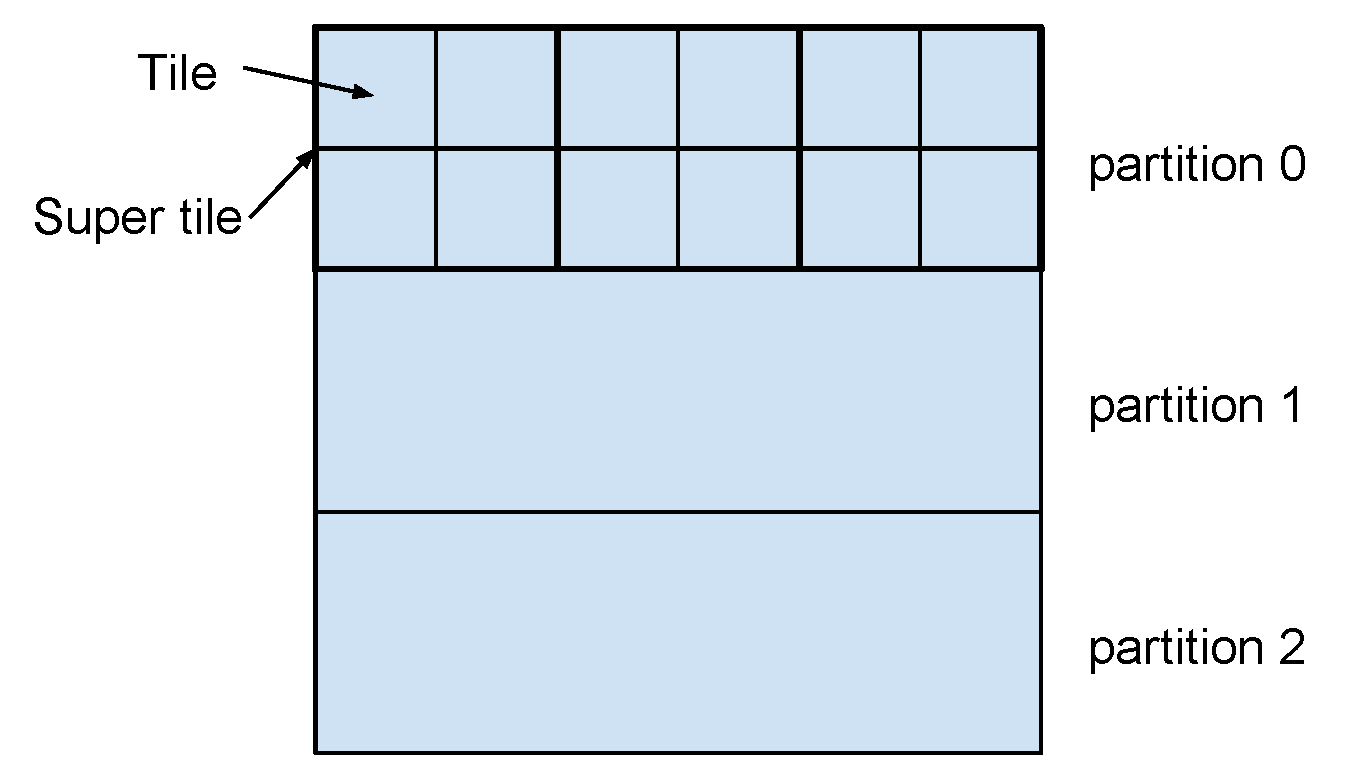
\includegraphics[scale=0.3]{./sparse_mat.pdf}
\caption{The format of a sparse matrix.}
\label{sparse_mat}
\end{figure}

To increase CPU cache hits, we deploy cache blocking \cite{Im04} and store
non-zero entries of a sparse matrix in tiles (Figure \ref{sparse_mat}).
When a tile is small, the rows from the input and output dense matrices
involved in the multiplication with the tile are always kept in the CPU cache
during the computation. The optimal tile size should fill the CPU cache
with the rows of the dense matrices involved in the multiplication with
the tile and is affected by the number of columns of the dense matrices,
specified by applications. Instead of generating a sparse matrix with
different tile sizes optimized for different numbers of columns in the dense
matrices, we use a relatively small tile size and rely on the runtime system
to optimize for different numbers of columns (in section \ref{sec:cpu}).
In semi-external memory, we expect that the dense matrices have a very small
number of columns in sparse matrix multiplication. Therefore, we
use the tile size of $16K \times 16K$ by default to balance the matrix storage
size and the adaptibility to different numbers of columns.

\begin{figure}
\centering
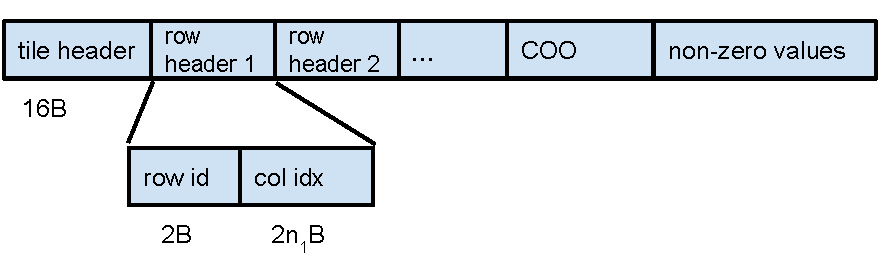
\includegraphics[scale=0.5]{./tile_format.pdf}
\caption{The storage format of a tile in a sparse matrix.}
\label{tile_format}
\end{figure}

To reduce the overall storage size of a sparse matrix, we use a compact format
to store non-zero entries in a tile. In very sparse matrices such as
many real-world graphs, many rows in a tile do not have any non-zero entries.
The CSR (CSC) format requires an entry for each row (column) in the row
(column) index. Therefore, the CSR or CSC format wastes space when storing elements
in a tile. Instead, we only keep data for rows with non-zero entries in a tile
shown in Figure \ref{tile_format} and refer to this format as SCSR (Super
Compressed Row Storage). This format maintains a row header for each non-empty
row. A row header has an identifier to indicate the row number, followed by
column indices. 
The most significant bit of the identifier is always set to 1, while the most
significant bit of a column index entry is always set to 0. As such, we can easily
distinguish a row identifier from a column index entry and determine the end
of a row. Thanks to the small size of a tile, we use two bytes to further store a row
number and a column index entry to reduce the storage size. Since the most
significant bit is used to indicate the beginning of a row, this format allows
a maximum tile size of $32K \times 32K$.

The SCSR format potentially results in many conditional jump CPU instructions
for sparse matrices with small cache blocking. As such, we hybrid SCSR and
the coordinate format (COO) to store non-zero entries in a tile to reduce
conditional jumps.
For real-world graphs, many rows in a cache tile have only one non-zero entry,
owing to the sparsity of the graphs and nearly random vertex connection.
Iterating over single-entry rows requires to test the end of a row for every
non-zero entry, which leads to many conditional jumps.
In contrast, COO is more suitable for storing these
single-entry rows. It does not increase the storage size but significantly
reduces the number of conditional jump instructions. As a result, we hybrid
SCSR and COO and store non-zero entries in the COO format behind the row headers
of SCSR (Figure \ref{tile_format}). All non-zero entries are
stored together at the end of a tile.

We organize tiles in a sparse matrix in tile rows and maintain a matrix index
for them. Each entry of the index stores the location of a tile row on SSDs
to facilitate random access
to tile rows. This is useful for parallelizing sparse matrix multiplication.
Because a tile contains thousands of rows, the matrix index requires a very
small storage size even for a billion-node graph. We keep the entire index
in memory during sparse matrix multiplication.

\subsection{Dense matrices}
Dense matrices in sparse matrix multiplication are tall-and-skinny matrices
with millions or even billions of rows but only a small number of columns.
The number of rows in a dense matrix is determined by the number of rows or
columns in a sparse matrix and the number of columns is determined by applications.
We keep the input dense matrix in memory, so its size governs memory consumption
of sparse matrix multiplication. To increase data locality in SpMM, the elements
in the dense matrices are stored in row-major order.
Given the limited amount of RAM in a machine,
the number of columns in a dense matrix has to be small.

For a non-uniform memory architecture (NUMA), we partition the input dense matrix
horizontally and store partitions evenly across NUMA nodes. The NUMA architecture
is prevalent in today's multi-processor servers, where each processor connects
to its own memory banks. Therefore, keeping partitions evenly across all NUMA
nodes helps to fully utilize the bandwidth of memory and inter-processor links.
For horizontal partitioning, we assign multiple contiguous rows in a row
interval to a partition, which is assigned to a NUMA node. A row interval
in a partition always has $2^i$ rows for efficiently locating a row
with bit operations. The row interval size is multiple of the tile size of
a sparse matrix so that multiplication on a tile only needs to access rows
from a single row interval.

%\begin{figure}
%\centering
%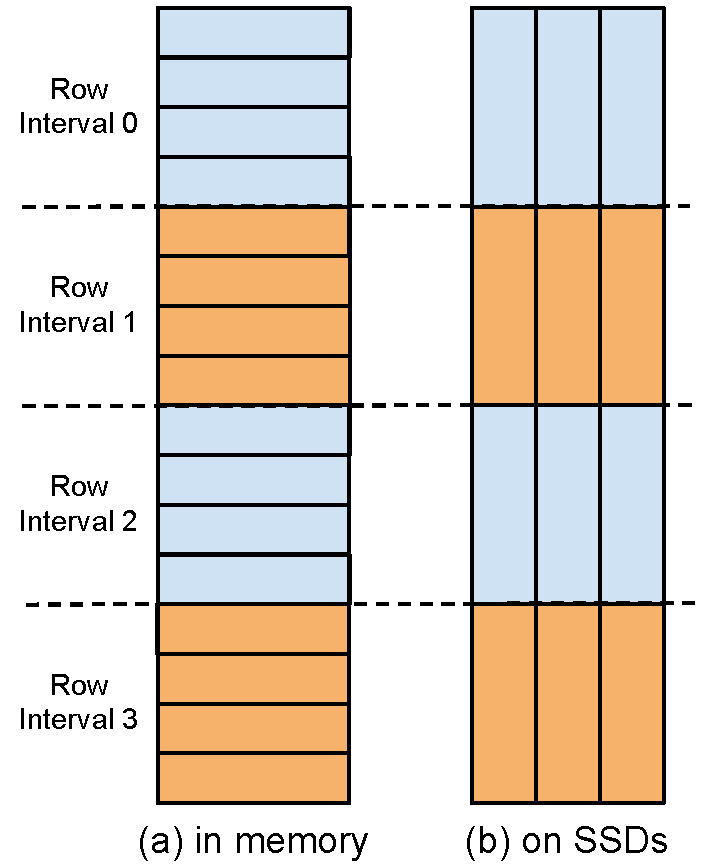
\includegraphics[scale=0.4]{./dense_matrix.pdf}
%\caption{The data layout of tall-and-skinny dense matrices. It is partitioned
%	horizontally into many row intervals.
%(a) In the input dense matrix of SpMM, row intervals are stored across NUMA nodes and
%elements are stored in the row-major order; (b) in the eigensolver, elements
%in a dense matrix inside a row interval are stored in the column-major order;
%(c) in NMF, a dense matrix is partitioned vertically first and in each partition,
%elements are stored in the row-major order.}
%\label{dense_mat}
%\end{figure}

\subsection{Semi-external memory}
With semi-external memory, we keep the sparse matrix on SSDs and keep the dense
matrix in memory for sparse matrix multiplication. To minimize memory
consumption, we keep only the input dense matrix in memory and
stream the output matrix to SSDs during the computation as necessary. We also stream
data in the sparse matrix from SSDs, which maximizes I/O throughput of the SSDs.

There are three options of keeping the output dense matrix. In applications
such as PageRank and many other graph
algorithms, dense matrices have only a few columns, so we can keep the output
dense matrix in memory for many machines. If a machine has insufficient
memory to keep the output dense matrix, we stream the output dense matrix
back to SSDs during the computation. As such, we significantly reduce I/O.

In some applications such as non-negative matrix factorization (Section
\ref{sec:apps}), even the input dense matrix cannot fit in memory. In this case,
we partition the input dense matrix vertically so
that each partition has complete columns of the original dense matrix and can
fit in memory. Each partition is stored in the row-major order to increase
data locality. For each partition, we perform sparse matrix multiplication
in semi-external memory as before and stream the output matrix to SSDs.
This approach requires $\lceil \frac{D}{M} \rceil$ passes over the sparse matrix,
where $D$ is the storage size of the input dense matrix and $M$ is the memory
size.

\subsection{Parallelization}
When parallelizing sparse matrix multiplication, we take into account
semi-external memory as well as the power-law distribution of non-zero entries
in each row of the sparse matrix.

We partition a sparse matrix horizontally for parallelization (Figure
\ref{sparse_mat}). Horizontal partitioning reduces interaction between threads.
A thread reads tile rows from SSDs asynchronously and processes them
independently. Once the tile rows
are ready in memory, the thread multiplies the tile rows with the input
dense matrix. The second benefit of horizontal partitioning is to reduce memory
consumption. Reducing memory consumption is essential for semi-external memory
sparse matrix dense matrix multiplication because keeping more columns in
the input dense matrix in memory can significantly reduce I/O from SSDs
(as discussed in Section \ref{sec:mem}). Horizontal partitioning ensures that
only the thread assigned with the tile rows need to allocate local memory buffers
for them. A thread needs to store the intermediate result in a local buffer to
reduce remote memory access in a NUMA machine when going through all the tiles
in the partition. Horizontal partitioning uses
a small matrix index to locate non-zero entries in the sparse matrix quickly.
With horizontal partitioning, we only need to locate tile rows. Therefore,
the matrix index is tiny even for a sparse matrix with billions of rows
and we can keep the entire matrix index in memory.

We maintain a global task queue for sparse matrix multiplication and a
thread gets one task at a time from the queue. A task may
indicates the computation on a \textit{super tile} row or a single tile row.
At the beginning of the computation, threads get larger tasks; when
the computation gets close to the end, threads get smaller tasks. This strategy
achieves good load balancing. The other benefit of maintaining a global
task queue is to maintain the global execution order, which becomes essential
when the output dense matrix needs to be written to SSDs. When a thread gets
a task, the final computation result from the task may be small. Instead of
writing the computation result immediately when it is generated, we delay
writes in order to merge
computation results from multiple threads and write them with a single I/O.
As such, we need to use the global task queue to ensure that all threads are
processing contiguous tile rows to help merge.

\subsection{Runtime CPU optimizations} \label{sec:cpu}
Even though the sparse matrix is constructed to reduce CPU cache misses,
we can perform further optimizations to speed up sparse matrix dense matrix
multiplication at runtime.

To better utilize CPU cache, we process tiles of a partition in
\textit{super tile}s (Figure \ref{sparse_mat}). The tile size of a sparse
matrix is specified when the sparse matrix image is created and is relatively
small to handle different numbers of columns in the dense matrices.
A \textit{super tile} is composed of tiles from multiple tile rows and its
size is determined at runtime by three factors: the number of columns
in the dense matrices, the CPU cache size and the number of threads that
share the CPU cache. An optimal size for a \textit{super tile} fills
the CPU cache with the rows from the dense matrices involved in
the computation with the \textit{super tile}.

In spite of nearly random edge connection in a real-world graph,
there exists regularity \dz{explain more?} that allows vectorization to improve performance
in sparse matrix dense matrix multiplication. For each non-zero entry, we
need to multiply it with the corresponding row from the input dense matrix
and add the result to the corresponding row in the output dense matrix.
These operations can be accomplished by the vector CPU instructions, such as
AVX \cite{avx}. The current implementation relies on GCC's auto-vectorization
to translate the C code to the vector CPU instructions by predefining the matrix
width in the code.

\subsection{I/O optimizations}
Semi-external memory sparse matrix multiplication results in sequential I/O
by streaming the sparse matrix from SSDs and potentially streaming the output
dense matrix to SSDs. For accessing fast SSDs, the overhead of operating systems
such as thread context switch and memory allocation becomes noticeable.
We need to tackle these obstacles in order to achieve the maximal I/O
throughput of fast SSDs.

The latency of a thread context switch undermines the sequential I/O throughput
of a high-speed SSD array.
%and it becomes critical to avoid thread context switch to gain I/O performance.
When a thread issues I/O and waits for I/O completion, the thread is switched
out. Once I/O is complete, the thread is rescheduled for execution and there is
latency for rescheduling. To reduce the effect of thread context switch,
an application thread issues asynchronous I/O and polls for I/O to avoid thread
context switches after completing all computation available to it.

When accessing a sparse matrix or a dense matrix from SSDs, we maintain a set of
memory buffers for I/O access to reduce the overhead of memory allocation.
We use large I/O to access matrices on SSDs to increase I/O throughput.
The operating system usually allocate a large memory buffer with \textit{mmap()}
and populates the buffer with physical pages when it is used. It is
computationally expensive to populate
large memory buffers frequently. When accessing high-throughput I/O devices,
such overhead can cause substantial performance loss. Therefore, we keep a set
of memory buffers allocated previously and reuse them for new I/O requests.
For accessing a sparse matrix, tile rows usually have differnt sizes, we resize
a previously allocated memory buffer if it is too small for a new I/O request.

\subsection{The impact of the memory size on I/O in semi-external memory}
\label{sec:mem}
The memory size has significant impact on I/O in semi-external memory.
The minimum memory requirement for semi-external memory sparse matrix
multiplication is $n c + \epsilon$, where $n$ is the number of rows
of the input dense matrix, $c$ is the element size of the dense matrix
and $\epsilon$ is the buffer size for part of the sparse matrix and the output
dense matrix. When a machine does not have sufficient memory to keep the entire
input dense matrix in memory, we need multiple passes on the sparse matrix to
perform sparse matrix multiplication. As such, a larger memory size reduces I/O
and for a fixed memory size, reducing memory consumption is
essential for semi-external memory.

When a machine does not have sufficient memory to keep the entire input dense
matrix, we should use the existing memory to keep as many columns in the input
dense matrix in memory as possible. Although we can cache part of the sparse
matrix,
keeping more columns of the input dense matrix in memory saves more I/O than
using the same amount of memory to cache the sparse matrix. Assume the input
dense matrix has $n$ rows and $k$ columns. The storage size of the sparse
matrix is $E$ bytes and the memory size is $M$ bytes. We further assume
we use $M'$ bytes to keep some columns of the dense matrices in memory
($M' < M$, ${n c k} \mod {M'} \equiv 0$)
and the remaining memory ($M - M'$) to cache the sparse matrix.
The amount of data in the sparse matrix read from SSDs is
\begin{equation*}
IO_{in} = \frac{n c k}{M'} [E - (M - M')]
\end{equation*}
Because $E > M$ in semi-external memory, we can minimize $IO_{in}$ by maximizing $M'$.
Therefore, using memory for the input dense matrix always results in a smaller
amount of I/O than using memory for caching sparse matrix.

As the number of columns from the input dense matrix kept in memory increases,
the bottleneck of the system
may switch. When we can keep only one column of the input dense matrix in memory,
the system may be I/O bound; when we can keep more columns of the dense matrix
in memory, the system will become CPU bound. Once the system becomes CPU bound,
the I/O complexity becomes irrelevant and the additional memory does not improve
the performance of sparse matrix multiplication further.

Our strategy results in the minimum amount of data written to SSDs. When the output
dense matrix cannot fit in memory, the maximum write is $N k$ for a square
sparse matrix.
In other words, the output matrix only needs to be written to SSDs at most once.
The additional memory in the system can be used to buffer part of the output
dense matrix to reduce the amount of data written to SSDs. Streaming the output
matrix directly to the subsequent matrix computation can also reduce data written
to SSDs.

\subsection{I/O complexity}
The semi-external memory (SEM) solution for sparse matrix multiplication leads
to no more I/O than the external-memory (EM) solution for many real-world graphs.

When a machine has sufficient memory to keep the entire input dense matrix
in memory, the SEM solution only needs to read the sparse matrix and the input
dense matrix once and write the output dense matrix once. This results in
a minimum amount of I/O. As such, the SEM solution does not cause more I/O
than any EM solutions.

When a machine has insufficient memory to keep the input dense matrix, the SEM
solution still leads to less I/O than the EM solution when
$E < n c k t$.
In this case, the SEM solution scans the sparse matrix multiple times.
\begin{equation*}
read_{SEM} = \frac{n c k}{M'} [E - (M - M')] + n c k
\end{equation*}
To minimize writes, the EM solution
scans the sparse matrix once but reads the input dense matrix multiple times.
Due to near vertex connection in real-world graphs, the EM solution needs to
read the entire input dense matrices each time. In the parallel setting,
the EM solution requires each thread to keep local memory buffers for portions
of the input and output dense matrices. Assume the EM solution keeps $j$ rows
from the input dense matrix and $i$ rows from the output dense matrix in memory
in each thread.
\begin{equation*}
(i c k + j c k) t = M => i < \frac{M}{c k t}
\end{equation*}
\begin{equation*}
read_{EM} = \frac{n}{i} n c k + E =>  read_{EM} > \frac{n^2 c^2 k^2 t}{M} + E
\end{equation*}
When $n c k < E < n c k t$, $read_{EM} > read_{SEM}$.
When $E \geq n c k$, $read_{EM} \geq read_{SEM}$ for any $t \geq 2$.

As such, the SEM solution in practice causes less I/O in many natural graphs.
For the natural graphs that we have seen, such as Twitter \cite{twitter},
the Page graph \cite{web_graph} and Friendster \cite{friendster}, the number
of edges is of $10-100 \times$ the number of vertices. Essentially,
natural graphs have sparse edge matrices. We target multi-core machines with
10s to 100s of threads. For most of our applications, $k$ is of size 1-30.
For very small $k$, the SEM
solution can keep the entire input dense matrix in memory and leads to minimum
I/O. For a relatively larger $k$, $E < n c k t$ holds
for most of natural graphs. Therefore, the SEM solution usually performs less
I/O than EM.

\section{Applications} \label{sec:apps}
We apply sparse matrix multiplication to three important applications widely
used in data mining and machine learning: PageRank \cite{pagerank},
eigendecomposition \cite{anasazi} and non-negative matrix factorization \cite{nmf}.
Each application demonstrates a a slightly different strategy of using memory
for sparse matrix multiplication.

\subsection{PageRank} \label{sec:pagerank}
PageRank is an algorithm to rank the Web pages by using hyperlinks between Web
pages. It was first used by Google and is identified as one of the top 10 data
mining algorithms \cite{top10}. PageRank is a representative of a set of graph
algorithms that can be expressed with sparse matrix multiplication or generalized
sparse matrix multiplication. Other important examples are label propagation
\cite{label_prop} and belief propagation \cite{Yedidia03}. The algorithm runs
iteratively and its update rule for each Web pages in an iteration is
\begin{equation*}
PR(u) = \frac{1-d}{N} + d \sum\limits_{v \in B(u)} \frac{PR(v)}{L(v)}
\end{equation*}
where $B(u)$ denotes the neighbor list of vertex $u$ and $L(v)$ denotes
the out-degree of vertex $v$. The PageRank algorithm is implemented with sparse
matrix multiplication (Figure \ref{code:pagerank}).


\begin{figure}
\centering
%\begin{minted}[mathescape, fontsize=\scriptsize,]{r}
\begin{lstlisting}
while (L1 >= epsilon && niters < max.niters) {
	pr2 <- d/N+(1-d)*(A %*% (pr1/out.deg))
	L1 <- sum(abs(pr1-pr2))
	pr1 <- pr2
	niters <- niters + 1
}
\end{lstlisting}
%\end{minted}
\caption{The implementation of PageRank with SpMM.}
\label{code:pagerank}
\end{figure}

Based on the memory size, we can place different data in memory to reduce I/O.
When the memory can only fit a single vector, each iteration needs
to write a vector to SSDs and read two vectors (the result from
the previous iteration and the degree vector) and the sparse matrix
from SSDs. When the memory can fit two vectors, the output vector can be kept
in memory, so each iteration needs to read the sparse matrix and the degree vector
and does not write any data to SSDs. As more memory can be used, we can
further keep the degree vector and even cache part of the sparse matrix.

\subsection{Eigendecomposition}
Eigendecomposition is another commonly
used application that requires sparse matrix multiplication. Many
algorithms \cite{Lanczos, IRLM, krylovschur} and frameworks
\cite{arpack, anasazi, slepc} have been developed to solve a large eigenvalue
problem.

We take advantage of the Anasazi eigensolver framework \cite{anasazi} and
replace its original matrix operations with our SEM sparse
matrix multiplication and external-memory dense matrix operations. To compute
eigenvalues of a $n \times n$ matrix, many eigenvalue algorithms for a large
sparse matrix require to construct a vector subspace with a sequence of
sparse matrix multiplication and each vector in the subspace has the length of $n$.
Due to the sparsity of many real-world graphs such as social networks,
the vector subspace requires substantial storage size and we keep
some of the vectors in the subspace on SSDs. In addition to sparse matrix
multiplication, eigensolvers perform some dense matrix operations on the subspace.
For example, eigensolvers need to orthogonalize the vectors in the subspace with
dense matrix multiplication. The Anasazi eigensolvers have block extension to
update multiple
vectors in the subspace simultaneously and thus require sparse matrix dense
matrix multiplication. The most efficient Anasazi eigensolver on sparse graphs
is the KrylovSchur eigensolver \cite{krylovschur}, which updates a small number
of vectors (1-4) in the subspace simultaneously. Zheng et al.
\cite{flasheigen} provides the details of extending the Anasazi eigensolver
with external-memory operations.

The choice of data placement for an eigensolver is a little different from
PageRank. If a machine has a small amount of memory, the memory should be
used to keep the input dense matrix. If a machine has more memory, we should
use it to buffer the output dense matrix. The dense matrices involved in
sparse matrix multiplication have a small number of columns in
the KrylovSchur eigensolver and usually can fit in memory. 
Additional memory should be used to buffer the vectors in the subspace
to reduce I/O for dense matrix operations.

\subsection{Non-negative matrix factorization}
Non-negative matrix factorization (NMF) \cite{nmf} is to find two non-negative
low-rank matrices $W$ and $H$ to approximate a matrix $A \approx WH$. NMF is
typically used to find factorization on sparse matrices. NMF has many applications
in machine learning
and data mining. A well-known example is collaborative filtering \cite{cf} in
recommender systems. NMF is also applied to graphs, for example, to find communities
\cite{yang13, wang11}.

Many algorithms are designed to solve NMF and here we describe an algorithm
\cite{nmf} that requires a sequence of sparse matrix multiplication.
The algorithm use multiplicative update rules and update matrices $W$ and $H$
alternately. In each iteration, the algorithm first fixes $W$ to update $H$
and then fixes $H$ to update $W$.
\begin{equation*}
H_{a\mu} \leftarrow H_{a\mu} \frac{{(W^TA)}_{a\mu}}{{(W^TWH)}_{a\mu}},
W_{ia} \leftarrow W_{ia} \frac{{(AH^T)}_{ia}}{{(WHH^T)}_{ia}}
\end{equation*}

We apply SEM sparse matrix multiplication to NMF differently
based on the memory size and the number of columns in $W$ and $H$. Due to
the sparsity of a graph, it is possible that the non-negative matrices $W$ and
$H$ may require the storage as large as the sparse matrix and no longer fit in
memory. Therefore, we need to partition $W$ and $H$ vertically and run multiple
sparse matrix multiplications to compute $W^TA$ and $AH^T$, if the memory is not
large enough to keep $W$ and $H$.

The choices of data placement for NMF are
shown as follows. If memory is small, all memory should be used to keep as many
columns in the input dense matrix as possible to reduce I/O. The original sparse
matrix multiplication is broken into multiple multiplications. We stream the output
dense matrices to SSDs and construct some of the input dense matrices for the next
sparse matrix multiplications in memory to reduce the latency of loading
the input dense matrix to memory. The additional memory in a machine can be used
to buffer the output dense matrix of sparse matrix multiplication.


\section{Experimental Evaluation}

We evaluate the performance of semi-external memory sparse matrix
multiplication on multiple real-world billion-scale graphs including a web-page
graph with 3.4 billion vertices. We first measure the performance of our
semi-external memory implementation and compare it with multiple in-memory
implementations: \textit{(i)} our in-memory implementation, \textit{(ii)} MKL
(\textit{mkl\_dcsrmm}) and \textit{(iii)} Trilinos Tpetra. We also demonstrate
the effectiveness of
CPU and I/O optimizations on sparse matrix multiplication.
We then evaluate the overall performance of the applications in Section
\ref{sec:apps} and demonstrate the impact of the memory size on the applications.

We conduct experiments on a non-uniform memory architecture machine with
four Intel Xeon E7-4860 processors, clocked at 2.6 GHz, and 1TB memory of
DDR3-1600. Each processor has 12 cores. The machine has three LSI SAS 9300-8e
host bus adapters (HBA) connected to a SuperMicro storage chassis, in which
24 OCZ Intrepid 3000 SSDs are installed. The 24 SSDs together are capable of
delivering 12 GB/s for read and 10 GB/s for write at maximum. The machine runs
Linux kernel v3.13.0. We use 48 threads for our in-memory and semi-external
implementation.

\begin{table}
\begin{center}
\footnotesize
\begin{tabular}{|c|c|c|c|c|}
\hline
Graph datasets & \# Vertices & \# Edges & Directed \\
\hline
Twitter \cite{twitter} & $42$M & $1.5$B & Yes \\
\hline
Friendster \cite{friendster} & $65$M & $1.7$B & No \\
\hline
Page graph \cite{web_graph} & $3.4$B & $129$B & Yes \\
\hline
RMAT-40 \cite{rmat} & 100M & 3.7B & Yes \& No \\
\hline
RMAT-160 \cite{rmat} & 100M & 14B & Yes \& No \\
\hline
\end{tabular}
\normalsize
\end{center}
\caption{Graph data sets. We construct a directed and undirected version for
both RMAT-40 and RMAT-160.}
\label{graphs}
\end{table}

We use the adjacency matrices of the graphs in Table \ref{graphs} for performance
evaluation. The smallest graph we use has 42 million vertices and 1.5 billion
edges. The largest graph is the Page graph with 3.4 billion vertices
and 129 billion edges, which is two orders of magnitude larger than the smallest
graphs. We generate two synthetic graphs with R-Mat \cite{rmat} to fill the size
gap between the smallest and largest graph. We construct a directed and
undirected version for each of the synthetic graphs because some applications
in Section \ref{sec:apps} run on directed graphs and others run on undirected
graphs. The real-world datasets are publically available and the synthetic
datasets are generated with the RMAT implementation in the \textit{boost}
library\footnote{We use the parameters of $a=0.57$, $b=0.19$, $c=0.19$,
$d=0.05$.}. We always use the undirected version of the synthetic graphs for
the performance evaluation of sparse matrix multiplication. The Page graph is
clustered by domain.

\subsection{The performance of sparse matrix multiplication}

We evaluate the performance of our semi-external memory implementation (SEM-SpMM)
and compare its performance with our in-memory implementation (IM-SpMM) and
other state-of-the-art in-memory implementations, including the ones in Intel MKL and
Trilinos Tpetra, on the graphs in Table \ref{graphs}. The MKL and Tpetra
implementations cannot run on the Page graph because its size exceeds the memory
capacity of our NUMA machine. We use Intel MKL 2015 and Trilinos v12.0.1 for
the experiments.

\subsubsection{SEM-SpMM vs. IM-SpMM}

\begin{figure}
	\begin{center}
		\footnotesize
		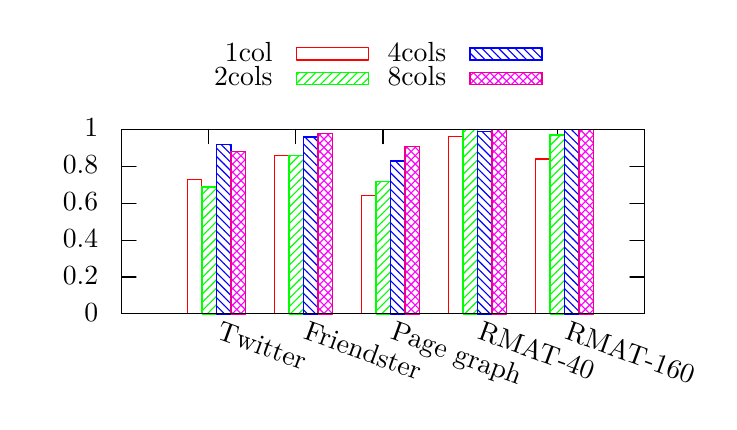
\begin{tikzpicture}[gnuplot]
%% generated with GNUPLOT 4.6p4 (Lua 5.1; terminal rev. 99, script rev. 100)
%% Mon 25 Jan 2016 02:13:31 PM EST
\path (0.000,0.000) rectangle (8.382,4.572);
\gpcolor{color=gp lt color border}
\gpsetlinetype{gp lt border}
\gpsetlinewidth{1.00}
\draw[gp path] (1.196,0.937)--(1.376,0.937);
\draw[gp path] (7.829,0.937)--(7.649,0.937);
\node[gp node right] at (1.012,0.937) { 0};
\draw[gp path] (1.196,1.405)--(1.376,1.405);
\draw[gp path] (7.829,1.405)--(7.649,1.405);
\node[gp node right] at (1.012,1.405) { 0.2};
\draw[gp path] (1.196,1.874)--(1.376,1.874);
\draw[gp path] (7.829,1.874)--(7.649,1.874);
\node[gp node right] at (1.012,1.874) { 0.4};
\draw[gp path] (1.196,2.342)--(1.376,2.342);
\draw[gp path] (7.829,2.342)--(7.649,2.342);
\node[gp node right] at (1.012,2.342) { 0.6};
\draw[gp path] (1.196,2.811)--(1.376,2.811);
\draw[gp path] (7.829,2.811)--(7.649,2.811);
\node[gp node right] at (1.012,2.811) { 0.8};
\draw[gp path] (1.196,3.279)--(1.376,3.279);
\draw[gp path] (7.829,3.279)--(7.649,3.279);
\node[gp node right] at (1.012,3.279) { 1};
\draw[gp path] (2.302,0.937)--(2.302,1.117);
\draw[gp path] (2.302,3.279)--(2.302,3.099);
\node[gp node left,rotate=-20] at (2.302,0.753) {Twitter};
\draw[gp path] (3.407,0.937)--(3.407,1.117);
\draw[gp path] (3.407,3.279)--(3.407,3.099);
\node[gp node left,rotate=-20] at (3.407,0.753) {Friendster};
\draw[gp path] (4.513,0.937)--(4.513,1.117);
\draw[gp path] (4.513,3.279)--(4.513,3.099);
\node[gp node left,rotate=-20] at (4.513,0.753) {Page graph};
\draw[gp path] (5.618,0.937)--(5.618,1.117);
\draw[gp path] (5.618,3.279)--(5.618,3.099);
\node[gp node left,rotate=-20] at (5.618,0.753) {RMAT-40};
\draw[gp path] (6.724,0.937)--(6.724,1.117);
\draw[gp path] (6.724,3.279)--(6.724,3.099);
\node[gp node left,rotate=-20] at (6.724,0.753) {RMAT-160};
\draw[gp path] (1.196,3.279)--(1.196,0.937)--(7.829,0.937)--(7.829,3.279)--cycle;
\node[gp node right] at (3.228,4.238) {1col};
\def\gpfillpath{(3.412,4.161)--(4.328,4.161)--(4.328,4.315)--(3.412,4.315)--cycle}
\gpfill{color=gpbgfillcolor} \gpfillpath;
\gpfill{color=gp lt color 0,gp pattern 0,pattern color=.} \gpfillpath;
\gpcolor{color=gp lt color 0}
\gpsetlinetype{gp lt plot 0}
\draw[gp path] (3.412,4.161)--(4.328,4.161)--(4.328,4.315)--(3.412,4.315)--cycle;
\def\gpfillpath{(2.025,0.937)--(2.210,0.937)--(2.210,2.648)--(2.025,2.648)--cycle}
\gpfill{color=gpbgfillcolor} \gpfillpath;
\gpfill{color=gp lt color 0,gp pattern 0,pattern color=.} \gpfillpath;
\draw[gp path] (2.025,0.937)--(2.025,2.647)--(2.209,2.647)--(2.209,0.937)--cycle;
\def\gpfillpath{(3.131,0.937)--(3.316,0.937)--(3.316,2.952)--(3.131,2.952)--cycle}
\gpfill{color=gpbgfillcolor} \gpfillpath;
\gpfill{color=gp lt color 0,gp pattern 0,pattern color=.} \gpfillpath;
\draw[gp path] (3.131,0.937)--(3.131,2.951)--(3.315,2.951)--(3.315,0.937)--cycle;
\def\gpfillpath{(4.236,0.937)--(4.421,0.937)--(4.421,2.437)--(4.236,2.437)--cycle}
\gpfill{color=gpbgfillcolor} \gpfillpath;
\gpfill{color=gp lt color 0,gp pattern 0,pattern color=.} \gpfillpath;
\draw[gp path] (4.236,0.937)--(4.236,2.436)--(4.420,2.436)--(4.420,0.937)--cycle;
\def\gpfillpath{(5.342,0.937)--(5.527,0.937)--(5.527,3.186)--(5.342,3.186)--cycle}
\gpfill{color=gpbgfillcolor} \gpfillpath;
\gpfill{color=gp lt color 0,gp pattern 0,pattern color=.} \gpfillpath;
\draw[gp path] (5.342,0.937)--(5.342,3.185)--(5.526,3.185)--(5.526,0.937)--cycle;
\def\gpfillpath{(6.447,0.937)--(6.632,0.937)--(6.632,2.905)--(6.447,2.905)--cycle}
\gpfill{color=gpbgfillcolor} \gpfillpath;
\gpfill{color=gp lt color 0,gp pattern 0,pattern color=.} \gpfillpath;
\draw[gp path] (6.447,0.937)--(6.447,2.904)--(6.631,2.904)--(6.631,0.937)--cycle;
\gpcolor{color=gp lt color border}
\node[gp node right] at (3.228,3.930) {2cols};
\def\gpfillpath{(3.412,3.853)--(4.328,3.853)--(4.328,4.007)--(3.412,4.007)--cycle}
\gpfill{color=gpbgfillcolor} \gpfillpath;
\gpfill{color=gp lt color 1,gp pattern 1,pattern color=.} \gpfillpath;
\gpcolor{color=gp lt color 1}
\gpsetlinetype{gp lt plot 1}
\draw[gp path] (3.412,3.853)--(4.328,3.853)--(4.328,4.007)--(3.412,4.007)--cycle;
\def\gpfillpath{(2.209,0.937)--(2.395,0.937)--(2.395,2.554)--(2.209,2.554)--cycle}
\gpfill{color=gpbgfillcolor} \gpfillpath;
\gpfill{color=gp lt color 1,gp pattern 1,pattern color=.} \gpfillpath;
\draw[gp path] (2.209,0.937)--(2.209,2.553)--(2.394,2.553)--(2.394,0.937)--cycle;
\def\gpfillpath{(3.315,0.937)--(3.500,0.937)--(3.500,2.952)--(3.315,2.952)--cycle}
\gpfill{color=gpbgfillcolor} \gpfillpath;
\gpfill{color=gp lt color 1,gp pattern 1,pattern color=.} \gpfillpath;
\draw[gp path] (3.315,0.937)--(3.315,2.951)--(3.499,2.951)--(3.499,0.937)--cycle;
\def\gpfillpath{(4.420,0.937)--(4.606,0.937)--(4.606,2.624)--(4.420,2.624)--cycle}
\gpfill{color=gpbgfillcolor} \gpfillpath;
\gpfill{color=gp lt color 1,gp pattern 1,pattern color=.} \gpfillpath;
\draw[gp path] (4.420,0.937)--(4.420,2.623)--(4.605,2.623)--(4.605,0.937)--cycle;
\def\gpfillpath{(5.526,0.937)--(5.711,0.937)--(5.711,3.280)--(5.526,3.280)--cycle}
\gpfill{color=gpbgfillcolor} \gpfillpath;
\gpfill{color=gp lt color 1,gp pattern 1,pattern color=.} \gpfillpath;
\draw[gp path] (5.526,0.937)--(5.526,3.279)--(5.710,3.279)--(5.710,0.937)--cycle;
\def\gpfillpath{(6.631,0.937)--(6.817,0.937)--(6.817,3.210)--(6.631,3.210)--cycle}
\gpfill{color=gpbgfillcolor} \gpfillpath;
\gpfill{color=gp lt color 1,gp pattern 1,pattern color=.} \gpfillpath;
\draw[gp path] (6.631,0.937)--(6.631,3.209)--(6.816,3.209)--(6.816,0.937)--cycle;
\gpcolor{color=gp lt color border}
\node[gp node right] at (5.432,4.238) {4cols};
\def\gpfillpath{(5.616,4.161)--(6.532,4.161)--(6.532,4.315)--(5.616,4.315)--cycle}
\gpfill{color=gpbgfillcolor} \gpfillpath;
\gpfill{color=gp lt color 2,gp pattern 2,pattern color=.} \gpfillpath;
\gpcolor{color=gp lt color 2}
\gpsetlinetype{gp lt plot 2}
\draw[gp path] (5.616,4.161)--(6.532,4.161)--(6.532,4.315)--(5.616,4.315)--cycle;
\def\gpfillpath{(2.394,0.937)--(2.579,0.937)--(2.579,3.093)--(2.394,3.093)--cycle}
\gpfill{color=gpbgfillcolor} \gpfillpath;
\gpfill{color=gp lt color 2,gp pattern 2,pattern color=.} \gpfillpath;
\draw[gp path] (2.394,0.937)--(2.394,3.092)--(2.578,3.092)--(2.578,0.937)--cycle;
\def\gpfillpath{(3.499,0.937)--(3.684,0.937)--(3.684,3.186)--(3.499,3.186)--cycle}
\gpfill{color=gpbgfillcolor} \gpfillpath;
\gpfill{color=gp lt color 2,gp pattern 2,pattern color=.} \gpfillpath;
\draw[gp path] (3.499,0.937)--(3.499,3.185)--(3.683,3.185)--(3.683,0.937)--cycle;
\def\gpfillpath{(4.605,0.937)--(4.790,0.937)--(4.790,2.882)--(4.605,2.882)--cycle}
\gpfill{color=gpbgfillcolor} \gpfillpath;
\gpfill{color=gp lt color 2,gp pattern 2,pattern color=.} \gpfillpath;
\draw[gp path] (4.605,0.937)--(4.605,2.881)--(4.789,2.881)--(4.789,0.937)--cycle;
\def\gpfillpath{(5.710,0.937)--(5.895,0.937)--(5.895,3.257)--(5.710,3.257)--cycle}
\gpfill{color=gpbgfillcolor} \gpfillpath;
\gpfill{color=gp lt color 2,gp pattern 2,pattern color=.} \gpfillpath;
\draw[gp path] (5.710,0.937)--(5.710,3.256)--(5.894,3.256)--(5.894,0.937)--cycle;
\def\gpfillpath{(6.816,0.937)--(7.001,0.937)--(7.001,3.280)--(6.816,3.280)--cycle}
\gpfill{color=gpbgfillcolor} \gpfillpath;
\gpfill{color=gp lt color 2,gp pattern 2,pattern color=.} \gpfillpath;
\draw[gp path] (6.816,0.937)--(6.816,3.279)--(7.000,3.279)--(7.000,0.937)--cycle;
\gpcolor{color=gp lt color border}
\node[gp node right] at (5.432,3.930) {8cols};
\def\gpfillpath{(5.616,3.853)--(6.532,3.853)--(6.532,4.007)--(5.616,4.007)--cycle}
\gpfill{color=gpbgfillcolor} \gpfillpath;
\gpfill{color=gp lt color 3,gp pattern 3,pattern color=.} \gpfillpath;
\gpcolor{color=gp lt color 3}
\gpsetlinetype{gp lt plot 3}
\draw[gp path] (5.616,3.853)--(6.532,3.853)--(6.532,4.007)--(5.616,4.007)--cycle;
\def\gpfillpath{(2.578,0.937)--(2.763,0.937)--(2.763,2.999)--(2.578,2.999)--cycle}
\gpfill{color=gpbgfillcolor} \gpfillpath;
\gpfill{color=gp lt color 3,gp pattern 3,pattern color=.} \gpfillpath;
\draw[gp path] (2.578,0.937)--(2.578,2.998)--(2.762,2.998)--(2.762,0.937)--cycle;
\def\gpfillpath{(3.683,0.937)--(3.869,0.937)--(3.869,3.233)--(3.683,3.233)--cycle}
\gpfill{color=gpbgfillcolor} \gpfillpath;
\gpfill{color=gp lt color 3,gp pattern 3,pattern color=.} \gpfillpath;
\draw[gp path] (3.683,0.937)--(3.683,3.232)--(3.868,3.232)--(3.868,0.937)--cycle;
\def\gpfillpath{(4.789,0.937)--(4.974,0.937)--(4.974,3.069)--(4.789,3.069)--cycle}
\gpfill{color=gpbgfillcolor} \gpfillpath;
\gpfill{color=gp lt color 3,gp pattern 3,pattern color=.} \gpfillpath;
\draw[gp path] (4.789,0.937)--(4.789,3.068)--(4.973,3.068)--(4.973,0.937)--cycle;
\def\gpfillpath{(5.894,0.937)--(6.080,0.937)--(6.080,3.280)--(5.894,3.280)--cycle}
\gpfill{color=gpbgfillcolor} \gpfillpath;
\gpfill{color=gp lt color 3,gp pattern 3,pattern color=.} \gpfillpath;
\draw[gp path] (5.894,0.937)--(5.894,3.279)--(6.079,3.279)--(6.079,0.937)--cycle;
\def\gpfillpath{(7.000,0.937)--(7.185,0.937)--(7.185,3.280)--(7.000,3.280)--cycle}
\gpfill{color=gpbgfillcolor} \gpfillpath;
\gpfill{color=gp lt color 3,gp pattern 3,pattern color=.} \gpfillpath;
\draw[gp path] (7.000,0.937)--(7.000,3.279)--(7.184,3.279)--(7.184,0.937)--cycle;
\gpcolor{color=gp lt color border}
\gpsetlinetype{gp lt border}
\draw[gp path] (1.196,3.279)--(1.196,0.937)--(7.829,0.937)--(7.829,3.279)--cycle;
%% coordinates of the plot area
\gpdefrectangularnode{gp plot 1}{\pgfpoint{1.196cm}{0.937cm}}{\pgfpoint{7.829cm}{3.279cm}}
\end{tikzpicture}
%% gnuplot variables

		\caption{The performance of SEM-SpMM with dense matrices of different
			numbers of columns, normalized to IM-SpMM for the dense matrix with
			the same number of columns.}
		\label{perf:spmm_comp}
	\end{center}
\end{figure}

We first compare the performance of SEM-SpMM against IM-SpMM on all graphs with
the input and output dense matrices stored in memory. In this case, the dense
matrices involved in SpMM have a small number of columns.

There is only a small performance penalty for semi-external memory (Figure
\ref{perf:spmm_comp}). The performance gap between IM-SpMM and SEM-SpMM
is affected by randomness of vertex connection. The gap is smaller if
vertex connection in a graph is more random. The Page graph is relatively
well clustered, so SpMM on this graph is less CPU-bound than others.
Even for the Page graph, SEM-SpMM gets 65\% performance of IM-SpMM.
The other factor of affecting the performance gap is the number of columns
in the dense matrices. The gap gets smaller as the number of columns in
the dense matrices increases. For all graphs, SEM-SpMM requires a very small
number of columns to become CPU-bound and achieve 100\% performance of IM-SpMM.

\subsubsection{SEM-SpMM vs. other in-memory SpMM}
In this section, we compare SEM-SpMM with the Intel MKL and Trilinos Tpetra
implementations. Intel MKL runs on shared-memory machines. Trilinos Tpetra can run in
both shared memory and distributed memory, so we measure its performance in
our 48-core NUMA machine as well as an EC2 cluster. We run Tpetra in the largest
EC2 instances r3.8xlarge, where each has 16 physical CPU cores and 244GB of RAM
and is optimized for memory-intensive applications. The EC2 instances are
connected with 10Gbps network in the same placement group.

\begin{figure}
	\footnotesize
	\centering
	\begin{subfigure}[b]{0.5\textwidth}
		\centering
		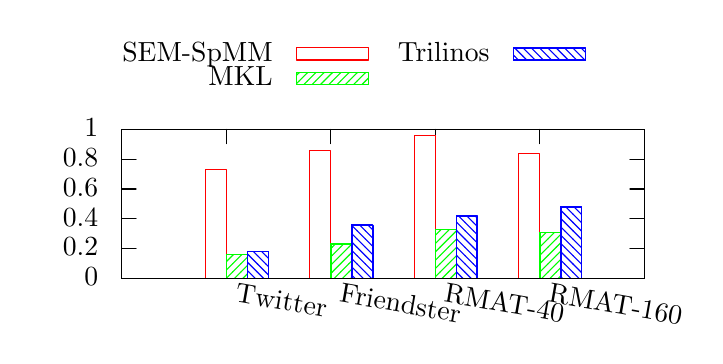
\begin{tikzpicture}[gnuplot]
%% generated with GNUPLOT 4.6p4 (Lua 5.1; terminal rev. 99, script rev. 100)
%% Mon 01 Feb 2016 07:59:05 PM EST
\path (0.000,0.000) rectangle (8.382,3.810);
\gpcolor{color=gp lt color border}
\gpsetlinetype{gp lt border}
\gpsetlinewidth{1.00}
\draw[gp path] (1.196,0.627)--(1.376,0.627);
\draw[gp path] (7.829,0.627)--(7.649,0.627);
\node[gp node right] at (1.012,0.627) { 0};
\draw[gp path] (1.196,1.005)--(1.376,1.005);
\draw[gp path] (7.829,1.005)--(7.649,1.005);
\node[gp node right] at (1.012,1.005) { 0.2};
\draw[gp path] (1.196,1.383)--(1.376,1.383);
\draw[gp path] (7.829,1.383)--(7.649,1.383);
\node[gp node right] at (1.012,1.383) { 0.4};
\draw[gp path] (1.196,1.761)--(1.376,1.761);
\draw[gp path] (7.829,1.761)--(7.649,1.761);
\node[gp node right] at (1.012,1.761) { 0.6};
\draw[gp path] (1.196,2.139)--(1.376,2.139);
\draw[gp path] (7.829,2.139)--(7.649,2.139);
\node[gp node right] at (1.012,2.139) { 0.8};
\draw[gp path] (1.196,2.517)--(1.376,2.517);
\draw[gp path] (7.829,2.517)--(7.649,2.517);
\node[gp node right] at (1.012,2.517) { 1};
\draw[gp path] (2.523,0.627)--(2.523,0.807);
\draw[gp path] (2.523,2.517)--(2.523,2.337);
\node[gp node left,rotate=-10] at (2.523,0.443) {Twitter};
\draw[gp path] (3.849,0.627)--(3.849,0.807);
\draw[gp path] (3.849,2.517)--(3.849,2.337);
\node[gp node left,rotate=-10] at (3.849,0.443) {Friendster};
\draw[gp path] (5.176,0.627)--(5.176,0.807);
\draw[gp path] (5.176,2.517)--(5.176,2.337);
\node[gp node left,rotate=-10] at (5.176,0.443) {RMAT-40};
\draw[gp path] (6.502,0.627)--(6.502,0.807);
\draw[gp path] (6.502,2.517)--(6.502,2.337);
\node[gp node left,rotate=-10] at (6.502,0.443) {RMAT-160};
\draw[gp path] (1.196,2.517)--(1.196,0.627)--(7.829,0.627)--(7.829,2.517)--cycle;
\node[gp node right] at (3.228,3.476) {SEM-SpMM};
\def\gpfillpath{(3.412,3.399)--(4.328,3.399)--(4.328,3.553)--(3.412,3.553)--cycle}
\gpfill{color=gpbgfillcolor} \gpfillpath;
\gpfill{color=gp lt color 0,gp pattern 0,pattern color=.} \gpfillpath;
\gpcolor{color=gp lt color 0}
\gpsetlinetype{gp lt plot 0}
\draw[gp path] (3.412,3.399)--(4.328,3.399)--(4.328,3.553)--(3.412,3.553)--cycle;
\def\gpfillpath{(2.257,0.627)--(2.524,0.627)--(2.524,2.008)--(2.257,2.008)--cycle}
\gpfill{color=gpbgfillcolor} \gpfillpath;
\gpfill{color=gp lt color 0,gp pattern 0,pattern color=.} \gpfillpath;
\draw[gp path] (2.257,0.627)--(2.257,2.007)--(2.523,2.007)--(2.523,0.627)--cycle;
\def\gpfillpath{(3.584,0.627)--(3.850,0.627)--(3.850,2.253)--(3.584,2.253)--cycle}
\gpfill{color=gpbgfillcolor} \gpfillpath;
\gpfill{color=gp lt color 0,gp pattern 0,pattern color=.} \gpfillpath;
\draw[gp path] (3.584,0.627)--(3.584,2.252)--(3.849,2.252)--(3.849,0.627)--cycle;
\def\gpfillpath{(4.910,0.627)--(5.177,0.627)--(5.177,2.442)--(4.910,2.442)--cycle}
\gpfill{color=gpbgfillcolor} \gpfillpath;
\gpfill{color=gp lt color 0,gp pattern 0,pattern color=.} \gpfillpath;
\draw[gp path] (4.910,0.627)--(4.910,2.441)--(5.176,2.441)--(5.176,0.627)--cycle;
\def\gpfillpath{(6.237,0.627)--(6.503,0.627)--(6.503,2.216)--(6.237,2.216)--cycle}
\gpfill{color=gpbgfillcolor} \gpfillpath;
\gpfill{color=gp lt color 0,gp pattern 0,pattern color=.} \gpfillpath;
\draw[gp path] (6.237,0.627)--(6.237,2.215)--(6.502,2.215)--(6.502,0.627)--cycle;
\gpcolor{color=gp lt color border}
\node[gp node right] at (3.228,3.168) {MKL};
\def\gpfillpath{(3.412,3.091)--(4.328,3.091)--(4.328,3.245)--(3.412,3.245)--cycle}
\gpfill{color=gpbgfillcolor} \gpfillpath;
\gpfill{color=gp lt color 1,gp pattern 1,pattern color=.} \gpfillpath;
\gpcolor{color=gp lt color 1}
\gpsetlinetype{gp lt plot 1}
\draw[gp path] (3.412,3.091)--(4.328,3.091)--(4.328,3.245)--(3.412,3.245)--cycle;
\def\gpfillpath{(2.523,0.627)--(2.789,0.627)--(2.789,0.930)--(2.523,0.930)--cycle}
\gpfill{color=gpbgfillcolor} \gpfillpath;
\gpfill{color=gp lt color 1,gp pattern 1,pattern color=.} \gpfillpath;
\draw[gp path] (2.523,0.627)--(2.523,0.929)--(2.788,0.929)--(2.788,0.627)--cycle;
\def\gpfillpath{(3.849,0.627)--(4.116,0.627)--(4.116,1.063)--(3.849,1.063)--cycle}
\gpfill{color=gpbgfillcolor} \gpfillpath;
\gpfill{color=gp lt color 1,gp pattern 1,pattern color=.} \gpfillpath;
\draw[gp path] (3.849,0.627)--(3.849,1.062)--(4.115,1.062)--(4.115,0.627)--cycle;
\def\gpfillpath{(5.176,0.627)--(5.442,0.627)--(5.442,1.252)--(5.176,1.252)--cycle}
\gpfill{color=gpbgfillcolor} \gpfillpath;
\gpfill{color=gp lt color 1,gp pattern 1,pattern color=.} \gpfillpath;
\draw[gp path] (5.176,0.627)--(5.176,1.251)--(5.441,1.251)--(5.441,0.627)--cycle;
\def\gpfillpath{(6.502,0.627)--(6.769,0.627)--(6.769,1.214)--(6.502,1.214)--cycle}
\gpfill{color=gpbgfillcolor} \gpfillpath;
\gpfill{color=gp lt color 1,gp pattern 1,pattern color=.} \gpfillpath;
\draw[gp path] (6.502,0.627)--(6.502,1.213)--(6.768,1.213)--(6.768,0.627)--cycle;
\gpcolor{color=gp lt color border}
\node[gp node right] at (5.984,3.476) {Trilinos};
\def\gpfillpath{(6.168,3.399)--(7.084,3.399)--(7.084,3.553)--(6.168,3.553)--cycle}
\gpfill{color=gpbgfillcolor} \gpfillpath;
\gpfill{color=gp lt color 2,gp pattern 2,pattern color=.} \gpfillpath;
\gpcolor{color=gp lt color 2}
\gpsetlinetype{gp lt plot 2}
\draw[gp path] (6.168,3.399)--(7.084,3.399)--(7.084,3.553)--(6.168,3.553)--cycle;
\def\gpfillpath{(2.788,0.627)--(3.054,0.627)--(3.054,0.968)--(2.788,0.968)--cycle}
\gpfill{color=gpbgfillcolor} \gpfillpath;
\gpfill{color=gp lt color 2,gp pattern 2,pattern color=.} \gpfillpath;
\draw[gp path] (2.788,0.627)--(2.788,0.967)--(3.053,0.967)--(3.053,0.627)--cycle;
\def\gpfillpath{(4.115,0.627)--(4.381,0.627)--(4.381,1.308)--(4.115,1.308)--cycle}
\gpfill{color=gpbgfillcolor} \gpfillpath;
\gpfill{color=gp lt color 2,gp pattern 2,pattern color=.} \gpfillpath;
\draw[gp path] (4.115,0.627)--(4.115,1.307)--(4.380,1.307)--(4.380,0.627)--cycle;
\def\gpfillpath{(5.441,0.627)--(5.707,0.627)--(5.707,1.422)--(5.441,1.422)--cycle}
\gpfill{color=gpbgfillcolor} \gpfillpath;
\gpfill{color=gp lt color 2,gp pattern 2,pattern color=.} \gpfillpath;
\draw[gp path] (5.441,0.627)--(5.441,1.421)--(5.706,1.421)--(5.706,0.627)--cycle;
\def\gpfillpath{(6.768,0.627)--(7.034,0.627)--(7.034,1.535)--(6.768,1.535)--cycle}
\gpfill{color=gpbgfillcolor} \gpfillpath;
\gpfill{color=gp lt color 2,gp pattern 2,pattern color=.} \gpfillpath;
\draw[gp path] (6.768,0.627)--(6.768,1.534)--(7.033,1.534)--(7.033,0.627)--cycle;
\gpcolor{color=gp lt color border}
\gpsetlinetype{gp lt border}
\draw[gp path] (1.196,2.517)--(1.196,0.627)--(7.829,0.627)--(7.829,2.517)--cycle;
%% coordinates of the plot area
\gpdefrectangularnode{gp plot 1}{\pgfpoint{1.196cm}{0.627cm}}{\pgfpoint{7.829cm}{2.517cm}}
\end{tikzpicture}
%% gnuplot variables

		\vspace{-10pt}
		\caption{SpMV}
		\label{perf:spmv}
	\end{subfigure}
	\begin{subfigure}[b]{0.5\textwidth}
		\centering
		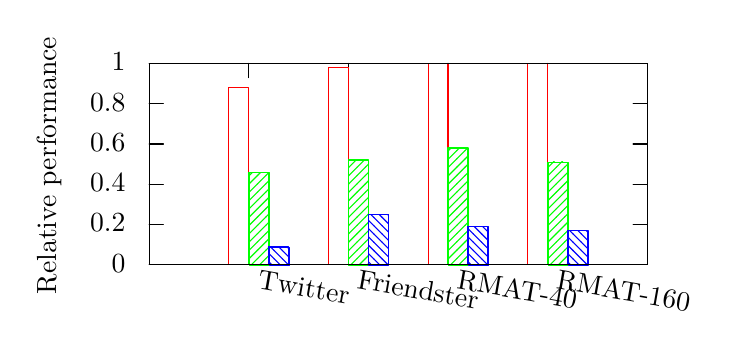
\begin{tikzpicture}[gnuplot]
%% generated with GNUPLOT 4.6p4 (Lua 5.1; terminal rev. 99, script rev. 100)
%% Tue 24 May 2016 11:19:54 AM EDT
\path (0.000,0.000) rectangle (8.382,3.556);
\gpcolor{color=gp lt color border}
\gpsetlinetype{gp lt border}
\gpsetlinewidth{1.00}
\draw[gp path] (1.504,0.627)--(1.684,0.627);
\draw[gp path] (7.829,0.627)--(7.649,0.627);
\node[gp node right] at (1.320,0.627) { 0};
\draw[gp path] (1.504,1.139)--(1.684,1.139);
\draw[gp path] (7.829,1.139)--(7.649,1.139);
\node[gp node right] at (1.320,1.139) { 0.2};
\draw[gp path] (1.504,1.651)--(1.684,1.651);
\draw[gp path] (7.829,1.651)--(7.649,1.651);
\node[gp node right] at (1.320,1.651) { 0.4};
\draw[gp path] (1.504,2.162)--(1.684,2.162);
\draw[gp path] (7.829,2.162)--(7.649,2.162);
\node[gp node right] at (1.320,2.162) { 0.6};
\draw[gp path] (1.504,2.674)--(1.684,2.674);
\draw[gp path] (7.829,2.674)--(7.649,2.674);
\node[gp node right] at (1.320,2.674) { 0.8};
\draw[gp path] (1.504,3.186)--(1.684,3.186);
\draw[gp path] (7.829,3.186)--(7.649,3.186);
\node[gp node right] at (1.320,3.186) { 1};
\draw[gp path] (2.769,0.627)--(2.769,0.807);
\draw[gp path] (2.769,3.186)--(2.769,3.006);
\node[gp node left,rotate=-10] at (2.769,0.443) {Twitter};
\draw[gp path] (4.034,0.627)--(4.034,0.807);
\draw[gp path] (4.034,3.186)--(4.034,3.006);
\node[gp node left,rotate=-10] at (4.034,0.443) {Friendster};
\draw[gp path] (5.299,0.627)--(5.299,0.807);
\draw[gp path] (5.299,3.186)--(5.299,3.006);
\node[gp node left,rotate=-10] at (5.299,0.443) {RMAT-40};
\draw[gp path] (6.564,0.627)--(6.564,0.807);
\draw[gp path] (6.564,3.186)--(6.564,3.006);
\node[gp node left,rotate=-10] at (6.564,0.443) {RMAT-160};
\draw[gp path] (1.504,3.186)--(1.504,0.627)--(7.829,0.627)--(7.829,3.186)--cycle;
\node[gp node center,rotate=-270] at (0.246,1.906) {Relative performance};
\def\gpfillpath{(2.516,0.627)--(2.770,0.627)--(2.770,2.880)--(2.516,2.880)--cycle}
\gpfill{color=gpbgfillcolor} \gpfillpath;
\gpfill{color=gp lt color 0,gp pattern 0,pattern color=.} \gpfillpath;
\gpcolor{color=gp lt color 0}
\gpsetlinetype{gp lt plot 0}
\draw[gp path] (2.516,0.627)--(2.516,2.879)--(2.769,2.879)--(2.769,0.627)--cycle;
\def\gpfillpath{(3.781,0.627)--(4.035,0.627)--(4.035,3.136)--(3.781,3.136)--cycle}
\gpfill{color=gpbgfillcolor} \gpfillpath;
\gpfill{color=gp lt color 0,gp pattern 0,pattern color=.} \gpfillpath;
\draw[gp path] (3.781,0.627)--(3.781,3.135)--(4.034,3.135)--(4.034,0.627)--cycle;
\def\gpfillpath{(5.046,0.627)--(5.300,0.627)--(5.300,3.187)--(5.046,3.187)--cycle}
\gpfill{color=gpbgfillcolor} \gpfillpath;
\gpfill{color=gp lt color 0,gp pattern 0,pattern color=.} \gpfillpath;
\draw[gp path] (5.046,0.627)--(5.046,3.186)--(5.299,3.186)--(5.299,0.627)--cycle;
\def\gpfillpath{(6.311,0.627)--(6.565,0.627)--(6.565,3.187)--(6.311,3.187)--cycle}
\gpfill{color=gpbgfillcolor} \gpfillpath;
\gpfill{color=gp lt color 0,gp pattern 0,pattern color=.} \gpfillpath;
\draw[gp path] (6.311,0.627)--(6.311,3.186)--(6.564,3.186)--(6.564,0.627)--cycle;
\def\gpfillpath{(2.769,0.627)--(3.023,0.627)--(3.023,1.805)--(2.769,1.805)--cycle}
\gpfill{color=gpbgfillcolor} \gpfillpath;
\gpfill{color=gp lt color 1,gp pattern 1,pattern color=.} \gpfillpath;
\gpcolor{color=gp lt color 1}
\gpsetlinetype{gp lt plot 1}
\draw[gp path] (2.769,0.627)--(2.769,1.804)--(3.022,1.804)--(3.022,0.627)--cycle;
\def\gpfillpath{(4.034,0.627)--(4.288,0.627)--(4.288,1.959)--(4.034,1.959)--cycle}
\gpfill{color=gpbgfillcolor} \gpfillpath;
\gpfill{color=gp lt color 1,gp pattern 1,pattern color=.} \gpfillpath;
\draw[gp path] (4.034,0.627)--(4.034,1.958)--(4.287,1.958)--(4.287,0.627)--cycle;
\def\gpfillpath{(5.299,0.627)--(5.553,0.627)--(5.553,2.112)--(5.299,2.112)--cycle}
\gpfill{color=gpbgfillcolor} \gpfillpath;
\gpfill{color=gp lt color 1,gp pattern 1,pattern color=.} \gpfillpath;
\draw[gp path] (5.299,0.627)--(5.299,2.111)--(5.552,2.111)--(5.552,0.627)--cycle;
\def\gpfillpath{(6.564,0.627)--(6.818,0.627)--(6.818,1.933)--(6.564,1.933)--cycle}
\gpfill{color=gpbgfillcolor} \gpfillpath;
\gpfill{color=gp lt color 1,gp pattern 1,pattern color=.} \gpfillpath;
\draw[gp path] (6.564,0.627)--(6.564,1.932)--(6.817,1.932)--(6.817,0.627)--cycle;
\def\gpfillpath{(3.022,0.627)--(3.276,0.627)--(3.276,0.858)--(3.022,0.858)--cycle}
\gpfill{color=gpbgfillcolor} \gpfillpath;
\gpfill{color=gp lt color 2,gp pattern 2,pattern color=.} \gpfillpath;
\gpcolor{color=gp lt color 2}
\gpsetlinetype{gp lt plot 2}
\draw[gp path] (3.022,0.627)--(3.022,0.857)--(3.275,0.857)--(3.275,0.627)--cycle;
\def\gpfillpath{(4.287,0.627)--(4.541,0.627)--(4.541,1.268)--(4.287,1.268)--cycle}
\gpfill{color=gpbgfillcolor} \gpfillpath;
\gpfill{color=gp lt color 2,gp pattern 2,pattern color=.} \gpfillpath;
\draw[gp path] (4.287,0.627)--(4.287,1.267)--(4.540,1.267)--(4.540,0.627)--cycle;
\def\gpfillpath{(5.552,0.627)--(5.806,0.627)--(5.806,1.114)--(5.552,1.114)--cycle}
\gpfill{color=gpbgfillcolor} \gpfillpath;
\gpfill{color=gp lt color 2,gp pattern 2,pattern color=.} \gpfillpath;
\draw[gp path] (5.552,0.627)--(5.552,1.113)--(5.805,1.113)--(5.805,0.627)--cycle;
\def\gpfillpath{(6.817,0.627)--(7.071,0.627)--(7.071,1.063)--(6.817,1.063)--cycle}
\gpfill{color=gpbgfillcolor} \gpfillpath;
\gpfill{color=gp lt color 2,gp pattern 2,pattern color=.} \gpfillpath;
\draw[gp path] (6.817,0.627)--(6.817,1.062)--(7.070,1.062)--(7.070,0.627)--cycle;
\gpcolor{color=gp lt color border}
\gpsetlinetype{gp lt border}
\draw[gp path] (1.504,3.186)--(1.504,0.627)--(7.829,0.627)--(7.829,3.186)--cycle;
%% coordinates of the plot area
\gpdefrectangularnode{gp plot 1}{\pgfpoint{1.504cm}{0.627cm}}{\pgfpoint{7.829cm}{3.186cm}}
\end{tikzpicture}
%% gnuplot variables

		\vspace{-10pt}
		\caption{SpMM with a dense matrix of 8 columns.}
		\label{perf:spmm8}
	\end{subfigure}
	\vspace{3pt}
	\caption{The performance of different sparse matrix multiplication
		implementations on the 48-core machine normalized to IM-SpMM for
	the same graphs.}
	\label{perf:spmm}
\end{figure}

Our SEM-SpMM significantly outperforms Intel MKL and Trilinos Tpetra on the natural
graphs on our NUMA machine (Figure \ref{perf:spmm}). In this case, we compare
performance of our SEM-SpMM with Intel MKL and Trilinos Tpetra for both sparse matrix
vector multiplication (SpMV) and sparse matrix dense matrix multiplication (SpMM).
The Tpetra implementation is optimized for SpMV. Our SEM-SpMM still constantly
outperforms Tpetra by a factor of $2-3$ even for SpMV. The MKL implementation has
better optimizations for SpMM than Trilinos Tpetra. Our SEM-SpMM is still almost
twice as fast as MKL in SpMM with a dense matrix of eight columns.


SEM-SpMM only consumes a small fraction of memory compared with IM-SpMM and
other SpMM implementations (Figure \ref{perf:spmm_mem}). SEM-SpMM consumes
memory for the input dense matrix as well as per-thread local memory buffers
for the sparse matrix and the output dense matrix. When we use 48 threads for
SpMM, the memory used by local memory buffers in each thread is significant
but is relatively constant for different graph sizes. We only show
the memory consumption on the largest graph RMAT-160 in Figure \ref{perf:spmm}.
Despite considerable memory consumed by
local memory buffers for SEM-SpMM, SEM-SpMM uses about one tenth of the memory
used by IM-SpMM. We also observe that IM-SpMM consumes much less memory than
MKL and Tpetra owing to its compact format for sparse matrices.

\begin{figure}
	\begin{center}
		\footnotesize
		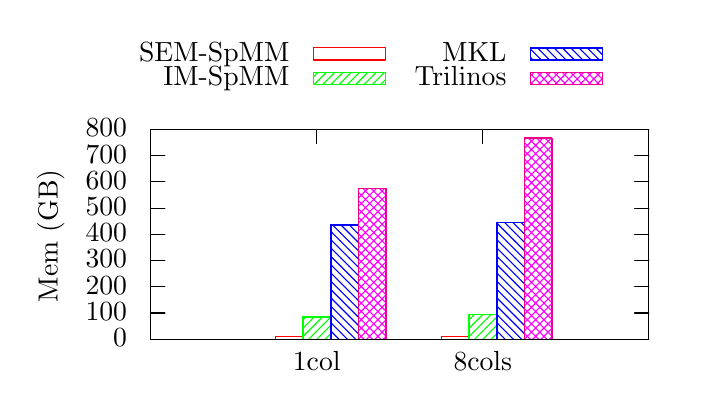
\begin{tikzpicture}[gnuplot]
%% generated with GNUPLOT 4.6p4 (Lua 5.1; terminal rev. 99, script rev. 100)
%% Mon 01 Feb 2016 08:04:07 PM EST
\path (0.000,0.000) rectangle (8.382,4.572);
\gpcolor{color=gp lt color border}
\gpsetlinetype{gp lt border}
\gpsetlinewidth{1.00}
\draw[gp path] (1.504,0.616)--(1.684,0.616);
\draw[gp path] (7.829,0.616)--(7.649,0.616);
\node[gp node right] at (1.320,0.616) { 0};
\draw[gp path] (1.504,0.949)--(1.684,0.949);
\draw[gp path] (7.829,0.949)--(7.649,0.949);
\node[gp node right] at (1.320,0.949) { 100};
\draw[gp path] (1.504,1.282)--(1.684,1.282);
\draw[gp path] (7.829,1.282)--(7.649,1.282);
\node[gp node right] at (1.320,1.282) { 200};
\draw[gp path] (1.504,1.615)--(1.684,1.615);
\draw[gp path] (7.829,1.615)--(7.649,1.615);
\node[gp node right] at (1.320,1.615) { 300};
\draw[gp path] (1.504,1.948)--(1.684,1.948);
\draw[gp path] (7.829,1.948)--(7.649,1.948);
\node[gp node right] at (1.320,1.948) { 400};
\draw[gp path] (1.504,2.280)--(1.684,2.280);
\draw[gp path] (7.829,2.280)--(7.649,2.280);
\node[gp node right] at (1.320,2.280) { 500};
\draw[gp path] (1.504,2.613)--(1.684,2.613);
\draw[gp path] (7.829,2.613)--(7.649,2.613);
\node[gp node right] at (1.320,2.613) { 600};
\draw[gp path] (1.504,2.946)--(1.684,2.946);
\draw[gp path] (7.829,2.946)--(7.649,2.946);
\node[gp node right] at (1.320,2.946) { 700};
\draw[gp path] (1.504,3.279)--(1.684,3.279);
\draw[gp path] (7.829,3.279)--(7.649,3.279);
\node[gp node right] at (1.320,3.279) { 800};
\draw[gp path] (3.612,0.616)--(3.612,0.796);
\draw[gp path] (3.612,3.279)--(3.612,3.099);
\node[gp node center] at (3.612,0.308) {1col};
\draw[gp path] (5.721,0.616)--(5.721,0.796);
\draw[gp path] (5.721,3.279)--(5.721,3.099);
\node[gp node center] at (5.721,0.308) {8cols};
\draw[gp path] (1.504,3.279)--(1.504,0.616)--(7.829,0.616)--(7.829,3.279)--cycle;
\node[gp node center,rotate=-270] at (0.246,1.947) {Mem (GB)};
\node[gp node right] at (3.382,4.238) {SEM-SpMM};
\def\gpfillpath{(3.566,4.161)--(4.482,4.161)--(4.482,4.315)--(3.566,4.315)--cycle}
\gpfill{color=gpbgfillcolor} \gpfillpath;
\gpfill{color=gp lt color 0,gp pattern 0,pattern color=.} \gpfillpath;
\gpcolor{color=gp lt color 0}
\gpsetlinetype{gp lt plot 0}
\draw[gp path] (3.566,4.161)--(4.482,4.161)--(4.482,4.315)--(3.566,4.315)--cycle;
\def\gpfillpath{(3.085,0.616)--(3.438,0.616)--(3.438,0.650)--(3.085,0.650)--cycle}
\gpfill{color=gpbgfillcolor} \gpfillpath;
\gpfill{color=gp lt color 0,gp pattern 0,pattern color=.} \gpfillpath;
\draw[gp path] (3.085,0.616)--(3.085,0.649)--(3.437,0.649)--(3.437,0.616)--cycle;
\def\gpfillpath{(5.194,0.616)--(5.546,0.616)--(5.546,0.654)--(5.194,0.654)--cycle}
\gpfill{color=gpbgfillcolor} \gpfillpath;
\gpfill{color=gp lt color 0,gp pattern 0,pattern color=.} \gpfillpath;
\draw[gp path] (5.194,0.616)--(5.194,0.653)--(5.545,0.653)--(5.545,0.616)--cycle;
\gpcolor{color=gp lt color border}
\node[gp node right] at (3.382,3.930) {IM-SpMM};
\def\gpfillpath{(3.566,3.853)--(4.482,3.853)--(4.482,4.007)--(3.566,4.007)--cycle}
\gpfill{color=gpbgfillcolor} \gpfillpath;
\gpfill{color=gp lt color 1,gp pattern 1,pattern color=.} \gpfillpath;
\gpcolor{color=gp lt color 1}
\gpsetlinetype{gp lt plot 1}
\draw[gp path] (3.566,3.853)--(4.482,3.853)--(4.482,4.007)--(3.566,4.007)--cycle;
\def\gpfillpath{(3.437,0.616)--(3.789,0.616)--(3.789,0.900)--(3.437,0.900)--cycle}
\gpfill{color=gpbgfillcolor} \gpfillpath;
\gpfill{color=gp lt color 1,gp pattern 1,pattern color=.} \gpfillpath;
\draw[gp path] (3.437,0.616)--(3.437,0.899)--(3.788,0.899)--(3.788,0.616)--cycle;
\def\gpfillpath{(5.545,0.616)--(5.897,0.616)--(5.897,0.930)--(5.545,0.930)--cycle}
\gpfill{color=gpbgfillcolor} \gpfillpath;
\gpfill{color=gp lt color 1,gp pattern 1,pattern color=.} \gpfillpath;
\draw[gp path] (5.545,0.616)--(5.545,0.929)--(5.896,0.929)--(5.896,0.616)--cycle;
\gpcolor{color=gp lt color border}
\node[gp node right] at (6.138,4.238) {MKL};
\def\gpfillpath{(6.322,4.161)--(7.238,4.161)--(7.238,4.315)--(6.322,4.315)--cycle}
\gpfill{color=gpbgfillcolor} \gpfillpath;
\gpfill{color=gp lt color 2,gp pattern 2,pattern color=.} \gpfillpath;
\gpcolor{color=gp lt color 2}
\gpsetlinetype{gp lt plot 2}
\draw[gp path] (6.322,4.161)--(7.238,4.161)--(7.238,4.315)--(6.322,4.315)--cycle;
\def\gpfillpath{(3.788,0.616)--(4.140,0.616)--(4.140,2.068)--(3.788,2.068)--cycle}
\gpfill{color=gpbgfillcolor} \gpfillpath;
\gpfill{color=gp lt color 2,gp pattern 2,pattern color=.} \gpfillpath;
\draw[gp path] (3.788,0.616)--(3.788,2.067)--(4.139,2.067)--(4.139,0.616)--cycle;
\def\gpfillpath{(5.896,0.616)--(6.249,0.616)--(6.249,2.102)--(5.896,2.102)--cycle}
\gpfill{color=gpbgfillcolor} \gpfillpath;
\gpfill{color=gp lt color 2,gp pattern 2,pattern color=.} \gpfillpath;
\draw[gp path] (5.896,0.616)--(5.896,2.101)--(6.248,2.101)--(6.248,0.616)--cycle;
\gpcolor{color=gp lt color border}
\node[gp node right] at (6.138,3.930) {Trilinos};
\def\gpfillpath{(6.322,3.853)--(7.238,3.853)--(7.238,4.007)--(6.322,4.007)--cycle}
\gpfill{color=gpbgfillcolor} \gpfillpath;
\gpfill{color=gp lt color 3,gp pattern 3,pattern color=.} \gpfillpath;
\gpcolor{color=gp lt color 3}
\gpsetlinetype{gp lt plot 3}
\draw[gp path] (6.322,3.853)--(7.238,3.853)--(7.238,4.007)--(6.322,4.007)--cycle;
\def\gpfillpath{(4.139,0.616)--(4.492,0.616)--(4.492,2.534)--(4.139,2.534)--cycle}
\gpfill{color=gpbgfillcolor} \gpfillpath;
\gpfill{color=gp lt color 3,gp pattern 3,pattern color=.} \gpfillpath;
\draw[gp path] (4.139,0.616)--(4.139,2.533)--(4.491,2.533)--(4.491,0.616)--cycle;
\def\gpfillpath{(6.248,0.616)--(6.600,0.616)--(6.600,3.173)--(6.248,3.173)--cycle}
\gpfill{color=gpbgfillcolor} \gpfillpath;
\gpfill{color=gp lt color 3,gp pattern 3,pattern color=.} \gpfillpath;
\draw[gp path] (6.248,0.616)--(6.248,3.172)--(6.599,3.172)--(6.599,0.616)--cycle;
\gpcolor{color=gp lt color border}
\gpsetlinetype{gp lt border}
\draw[gp path] (1.504,3.279)--(1.504,0.616)--(7.829,0.616)--(7.829,3.279)--cycle;
%% coordinates of the plot area
\gpdefrectangularnode{gp plot 1}{\pgfpoint{1.504cm}{0.616cm}}{\pgfpoint{7.829cm}{3.279cm}}
\end{tikzpicture}
%% gnuplot variables

		\caption{Memory consumption of different SpMM implementations on
		RMAT-160.}
		\label{perf:spmm_mem}
	\end{center}
\end{figure}

\begin{figure}
	\footnotesize
	\centering
	\begin{subfigure}[b]{0.5\textwidth}
		\centering
		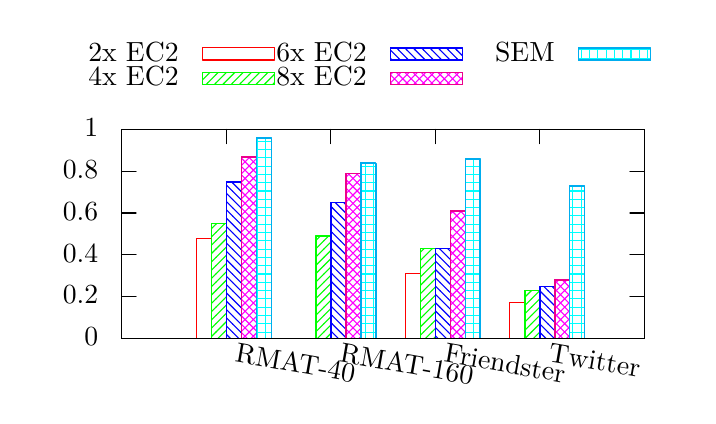
\begin{tikzpicture}[gnuplot]
%% generated with GNUPLOT 4.6p4 (Lua 5.1; terminal rev. 99, script rev. 100)
%% Fri 05 Feb 2016 01:43:18 PM EST
\path (0.000,0.000) rectangle (8.382,4.572);
\gpcolor{color=gp lt color border}
\gpsetlinetype{gp lt border}
\gpsetlinewidth{1.00}
\draw[gp path] (1.196,0.627)--(1.376,0.627);
\draw[gp path] (7.829,0.627)--(7.649,0.627);
\node[gp node right] at (1.012,0.627) { 0};
\draw[gp path] (1.196,1.157)--(1.376,1.157);
\draw[gp path] (7.829,1.157)--(7.649,1.157);
\node[gp node right] at (1.012,1.157) { 0.2};
\draw[gp path] (1.196,1.688)--(1.376,1.688);
\draw[gp path] (7.829,1.688)--(7.649,1.688);
\node[gp node right] at (1.012,1.688) { 0.4};
\draw[gp path] (1.196,2.218)--(1.376,2.218);
\draw[gp path] (7.829,2.218)--(7.649,2.218);
\node[gp node right] at (1.012,2.218) { 0.6};
\draw[gp path] (1.196,2.749)--(1.376,2.749);
\draw[gp path] (7.829,2.749)--(7.649,2.749);
\node[gp node right] at (1.012,2.749) { 0.8};
\draw[gp path] (1.196,3.279)--(1.376,3.279);
\draw[gp path] (7.829,3.279)--(7.649,3.279);
\node[gp node right] at (1.012,3.279) { 1};
\draw[gp path] (2.523,0.627)--(2.523,0.807);
\draw[gp path] (2.523,3.279)--(2.523,3.099);
\node[gp node left,rotate=-10] at (2.523,0.443) {RMAT-40};
\draw[gp path] (3.849,0.627)--(3.849,0.807);
\draw[gp path] (3.849,3.279)--(3.849,3.099);
\node[gp node left,rotate=-10] at (3.849,0.443) {RMAT-160};
\draw[gp path] (5.176,0.627)--(5.176,0.807);
\draw[gp path] (5.176,3.279)--(5.176,3.099);
\node[gp node left,rotate=-10] at (5.176,0.443) {Friendster};
\draw[gp path] (6.502,0.627)--(6.502,0.807);
\draw[gp path] (6.502,3.279)--(6.502,3.099);
\node[gp node left,rotate=-10] at (6.502,0.443) {Twitter};
\draw[gp path] (1.196,3.279)--(1.196,0.627)--(7.829,0.627)--(7.829,3.279)--cycle;
\node[gp node right] at (2.034,4.238) {2x EC2};
\def\gpfillpath{(2.218,4.161)--(3.134,4.161)--(3.134,4.315)--(2.218,4.315)--cycle}
\gpfill{color=gpbgfillcolor} \gpfillpath;
\gpfill{color=gp lt color 0,gp pattern 0,pattern color=.} \gpfillpath;
\gpcolor{color=gp lt color 0}
\gpsetlinetype{gp lt plot 0}
\draw[gp path] (2.218,4.161)--(3.134,4.161)--(3.134,4.315)--(2.218,4.315)--cycle;
\def\gpfillpath{(2.144,0.627)--(2.334,0.627)--(2.334,1.901)--(2.144,1.901)--cycle}
\gpfill{color=gpbgfillcolor} \gpfillpath;
\gpfill{color=gp lt color 0,gp pattern 0,pattern color=.} \gpfillpath;
\draw[gp path] (2.144,0.627)--(2.144,1.900)--(2.333,1.900)--(2.333,0.627)--cycle;
\def\gpfillpath{(4.797,0.627)--(4.987,0.627)--(4.987,1.450)--(4.797,1.450)--cycle}
\gpfill{color=gpbgfillcolor} \gpfillpath;
\gpfill{color=gp lt color 0,gp pattern 0,pattern color=.} \gpfillpath;
\draw[gp path] (4.797,0.627)--(4.797,1.449)--(4.986,1.449)--(4.986,0.627)--cycle;
\def\gpfillpath{(6.123,0.627)--(6.314,0.627)--(6.314,1.079)--(6.123,1.079)--cycle}
\gpfill{color=gpbgfillcolor} \gpfillpath;
\gpfill{color=gp lt color 0,gp pattern 0,pattern color=.} \gpfillpath;
\draw[gp path] (6.123,0.627)--(6.123,1.078)--(6.313,1.078)--(6.313,0.627)--cycle;
\gpcolor{color=gp lt color border}
\node[gp node right] at (2.034,3.930) {4x EC2};
\def\gpfillpath{(2.218,3.853)--(3.134,3.853)--(3.134,4.007)--(2.218,4.007)--cycle}
\gpfill{color=gpbgfillcolor} \gpfillpath;
\gpfill{color=gp lt color 1,gp pattern 1,pattern color=.} \gpfillpath;
\gpcolor{color=gp lt color 1}
\gpsetlinetype{gp lt plot 1}
\draw[gp path] (2.218,3.853)--(3.134,3.853)--(3.134,4.007)--(2.218,4.007)--cycle;
\def\gpfillpath{(2.333,0.627)--(2.524,0.627)--(2.524,2.087)--(2.333,2.087)--cycle}
\gpfill{color=gpbgfillcolor} \gpfillpath;
\gpfill{color=gp lt color 1,gp pattern 1,pattern color=.} \gpfillpath;
\draw[gp path] (2.333,0.627)--(2.333,2.086)--(2.523,2.086)--(2.523,0.627)--cycle;
\def\gpfillpath{(3.660,0.627)--(3.850,0.627)--(3.850,1.927)--(3.660,1.927)--cycle}
\gpfill{color=gpbgfillcolor} \gpfillpath;
\gpfill{color=gp lt color 1,gp pattern 1,pattern color=.} \gpfillpath;
\draw[gp path] (3.660,0.627)--(3.660,1.926)--(3.849,1.926)--(3.849,0.627)--cycle;
\def\gpfillpath{(4.986,0.627)--(5.177,0.627)--(5.177,1.768)--(4.986,1.768)--cycle}
\gpfill{color=gpbgfillcolor} \gpfillpath;
\gpfill{color=gp lt color 1,gp pattern 1,pattern color=.} \gpfillpath;
\draw[gp path] (4.986,0.627)--(4.986,1.767)--(5.176,1.767)--(5.176,0.627)--cycle;
\def\gpfillpath{(6.313,0.627)--(6.503,0.627)--(6.503,1.238)--(6.313,1.238)--cycle}
\gpfill{color=gpbgfillcolor} \gpfillpath;
\gpfill{color=gp lt color 1,gp pattern 1,pattern color=.} \gpfillpath;
\draw[gp path] (6.313,0.627)--(6.313,1.237)--(6.502,1.237)--(6.502,0.627)--cycle;
\gpcolor{color=gp lt color border}
\node[gp node right] at (4.422,4.238) {6x EC2};
\def\gpfillpath{(4.606,4.161)--(5.522,4.161)--(5.522,4.315)--(4.606,4.315)--cycle}
\gpfill{color=gpbgfillcolor} \gpfillpath;
\gpfill{color=gp lt color 2,gp pattern 2,pattern color=.} \gpfillpath;
\gpcolor{color=gp lt color 2}
\gpsetlinetype{gp lt plot 2}
\draw[gp path] (4.606,4.161)--(5.522,4.161)--(5.522,4.315)--(4.606,4.315)--cycle;
\def\gpfillpath{(2.523,0.627)--(2.713,0.627)--(2.713,2.617)--(2.523,2.617)--cycle}
\gpfill{color=gpbgfillcolor} \gpfillpath;
\gpfill{color=gp lt color 2,gp pattern 2,pattern color=.} \gpfillpath;
\draw[gp path] (2.523,0.627)--(2.523,2.616)--(2.712,2.616)--(2.712,0.627)--cycle;
\def\gpfillpath{(3.849,0.627)--(4.040,0.627)--(4.040,2.352)--(3.849,2.352)--cycle}
\gpfill{color=gpbgfillcolor} \gpfillpath;
\gpfill{color=gp lt color 2,gp pattern 2,pattern color=.} \gpfillpath;
\draw[gp path] (3.849,0.627)--(3.849,2.351)--(4.039,2.351)--(4.039,0.627)--cycle;
\def\gpfillpath{(5.176,0.627)--(5.366,0.627)--(5.366,1.768)--(5.176,1.768)--cycle}
\gpfill{color=gpbgfillcolor} \gpfillpath;
\gpfill{color=gp lt color 2,gp pattern 2,pattern color=.} \gpfillpath;
\draw[gp path] (5.176,0.627)--(5.176,1.767)--(5.365,1.767)--(5.365,0.627)--cycle;
\def\gpfillpath{(6.502,0.627)--(6.693,0.627)--(6.693,1.291)--(6.502,1.291)--cycle}
\gpfill{color=gpbgfillcolor} \gpfillpath;
\gpfill{color=gp lt color 2,gp pattern 2,pattern color=.} \gpfillpath;
\draw[gp path] (6.502,0.627)--(6.502,1.290)--(6.692,1.290)--(6.692,0.627)--cycle;
\gpcolor{color=gp lt color border}
\node[gp node right] at (4.422,3.930) {8x EC2};
\def\gpfillpath{(4.606,3.853)--(5.522,3.853)--(5.522,4.007)--(4.606,4.007)--cycle}
\gpfill{color=gpbgfillcolor} \gpfillpath;
\gpfill{color=gp lt color 3,gp pattern 3,pattern color=.} \gpfillpath;
\gpcolor{color=gp lt color 3}
\gpsetlinetype{gp lt plot 3}
\draw[gp path] (4.606,3.853)--(5.522,3.853)--(5.522,4.007)--(4.606,4.007)--cycle;
\def\gpfillpath{(2.712,0.627)--(2.903,0.627)--(2.903,2.935)--(2.712,2.935)--cycle}
\gpfill{color=gpbgfillcolor} \gpfillpath;
\gpfill{color=gp lt color 3,gp pattern 3,pattern color=.} \gpfillpath;
\draw[gp path] (2.712,0.627)--(2.712,2.934)--(2.902,2.934)--(2.902,0.627)--cycle;
\def\gpfillpath{(4.039,0.627)--(4.229,0.627)--(4.229,2.723)--(4.039,2.723)--cycle}
\gpfill{color=gpbgfillcolor} \gpfillpath;
\gpfill{color=gp lt color 3,gp pattern 3,pattern color=.} \gpfillpath;
\draw[gp path] (4.039,0.627)--(4.039,2.722)--(4.228,2.722)--(4.228,0.627)--cycle;
\def\gpfillpath{(5.365,0.627)--(5.556,0.627)--(5.556,2.246)--(5.365,2.246)--cycle}
\gpfill{color=gpbgfillcolor} \gpfillpath;
\gpfill{color=gp lt color 3,gp pattern 3,pattern color=.} \gpfillpath;
\draw[gp path] (5.365,0.627)--(5.365,2.245)--(5.555,2.245)--(5.555,0.627)--cycle;
\def\gpfillpath{(6.692,0.627)--(6.882,0.627)--(6.882,1.371)--(6.692,1.371)--cycle}
\gpfill{color=gpbgfillcolor} \gpfillpath;
\gpfill{color=gp lt color 3,gp pattern 3,pattern color=.} \gpfillpath;
\draw[gp path] (6.692,0.627)--(6.692,1.370)--(6.881,1.370)--(6.881,0.627)--cycle;
\gpcolor{color=gp lt color border}
\node[gp node right] at (6.810,4.238) {SEM};
\def\gpfillpath{(6.994,4.161)--(7.910,4.161)--(7.910,4.315)--(6.994,4.315)--cycle}
\gpfill{color=gpbgfillcolor} \gpfillpath;
\gpfill{color=gp lt color 4,gp pattern 4,pattern color=.} \gpfillpath;
\gpcolor{color=gp lt color 4}
\gpsetlinetype{gp lt plot 4}
\draw[gp path] (6.994,4.161)--(7.910,4.161)--(7.910,4.315)--(6.994,4.315)--cycle;
\def\gpfillpath{(2.902,0.627)--(3.092,0.627)--(3.092,3.174)--(2.902,3.174)--cycle}
\gpfill{color=gpbgfillcolor} \gpfillpath;
\gpfill{color=gp lt color 4,gp pattern 4,pattern color=.} \gpfillpath;
\draw[gp path] (2.902,0.627)--(2.902,3.173)--(3.091,3.173)--(3.091,0.627)--cycle;
\def\gpfillpath{(4.228,0.627)--(4.419,0.627)--(4.419,2.856)--(4.228,2.856)--cycle}
\gpfill{color=gpbgfillcolor} \gpfillpath;
\gpfill{color=gp lt color 4,gp pattern 4,pattern color=.} \gpfillpath;
\draw[gp path] (4.228,0.627)--(4.228,2.855)--(4.418,2.855)--(4.418,0.627)--cycle;
\def\gpfillpath{(5.555,0.627)--(5.745,0.627)--(5.745,2.909)--(5.555,2.909)--cycle}
\gpfill{color=gpbgfillcolor} \gpfillpath;
\gpfill{color=gp lt color 4,gp pattern 4,pattern color=.} \gpfillpath;
\draw[gp path] (5.555,0.627)--(5.555,2.908)--(5.744,2.908)--(5.744,0.627)--cycle;
\def\gpfillpath{(6.881,0.627)--(7.072,0.627)--(7.072,2.564)--(6.881,2.564)--cycle}
\gpfill{color=gpbgfillcolor} \gpfillpath;
\gpfill{color=gp lt color 4,gp pattern 4,pattern color=.} \gpfillpath;
\draw[gp path] (6.881,0.627)--(6.881,2.563)--(7.071,2.563)--(7.071,0.627)--cycle;
\gpcolor{color=gp lt color border}
\gpsetlinetype{gp lt border}
\draw[gp path] (1.196,3.279)--(1.196,0.627)--(7.829,0.627)--(7.829,3.279)--cycle;
%% coordinates of the plot area
\gpdefrectangularnode{gp plot 1}{\pgfpoint{1.196cm}{0.627cm}}{\pgfpoint{7.829cm}{3.279cm}}
\end{tikzpicture}
%% gnuplot variables

		\vspace{-10pt}
		\caption{SpMV}
		\label{perf:ec2:spmv}
	\end{subfigure}
	\begin{subfigure}[b]{0.5\textwidth}
		\centering
		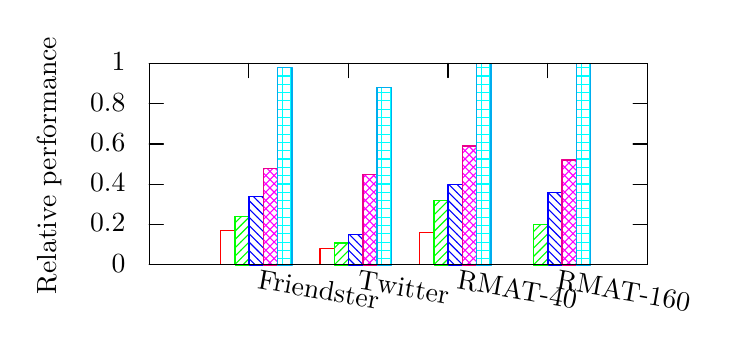
\begin{tikzpicture}[gnuplot]
%% generated with GNUPLOT 4.6p4 (Lua 5.1; terminal rev. 99, script rev. 100)
%% Thu 02 Jun 2016 05:02:43 PM EDT
\path (0.000,0.000) rectangle (8.382,3.556);
\gpcolor{color=gp lt color border}
\gpsetlinetype{gp lt border}
\gpsetlinewidth{1.00}
\draw[gp path] (1.504,0.627)--(1.684,0.627);
\draw[gp path] (7.829,0.627)--(7.649,0.627);
\node[gp node right] at (1.320,0.627) { 0};
\draw[gp path] (1.504,1.139)--(1.684,1.139);
\draw[gp path] (7.829,1.139)--(7.649,1.139);
\node[gp node right] at (1.320,1.139) { 0.2};
\draw[gp path] (1.504,1.651)--(1.684,1.651);
\draw[gp path] (7.829,1.651)--(7.649,1.651);
\node[gp node right] at (1.320,1.651) { 0.4};
\draw[gp path] (1.504,2.162)--(1.684,2.162);
\draw[gp path] (7.829,2.162)--(7.649,2.162);
\node[gp node right] at (1.320,2.162) { 0.6};
\draw[gp path] (1.504,2.674)--(1.684,2.674);
\draw[gp path] (7.829,2.674)--(7.649,2.674);
\node[gp node right] at (1.320,2.674) { 0.8};
\draw[gp path] (1.504,3.186)--(1.684,3.186);
\draw[gp path] (7.829,3.186)--(7.649,3.186);
\node[gp node right] at (1.320,3.186) { 1};
\draw[gp path] (2.769,0.627)--(2.769,0.807);
\draw[gp path] (2.769,3.186)--(2.769,3.006);
\node[gp node left,rotate=-10] at (2.769,0.443) {Friendster};
\draw[gp path] (4.034,0.627)--(4.034,0.807);
\draw[gp path] (4.034,3.186)--(4.034,3.006);
\node[gp node left,rotate=-10] at (4.034,0.443) {Twitter};
\draw[gp path] (5.299,0.627)--(5.299,0.807);
\draw[gp path] (5.299,3.186)--(5.299,3.006);
\node[gp node left,rotate=-10] at (5.299,0.443) {RMAT-40};
\draw[gp path] (6.564,0.627)--(6.564,0.807);
\draw[gp path] (6.564,3.186)--(6.564,3.006);
\node[gp node left,rotate=-10] at (6.564,0.443) {RMAT-160};
\draw[gp path] (1.504,3.186)--(1.504,0.627)--(7.829,0.627)--(7.829,3.186)--cycle;
\node[gp node center,rotate=-270] at (0.246,1.906) {Relative performance};
\def\gpfillpath{(2.408,0.627)--(2.589,0.627)--(2.589,1.063)--(2.408,1.063)--cycle}
\gpfill{color=gpbgfillcolor} \gpfillpath;
\gpfill{color=gp lt color 0,gp pattern 0,pattern color=.} \gpfillpath;
\gpcolor{color=gp lt color 0}
\gpsetlinetype{gp lt plot 0}
\draw[gp path] (2.408,0.627)--(2.408,1.062)--(2.588,1.062)--(2.588,0.627)--cycle;
\def\gpfillpath{(3.673,0.627)--(3.854,0.627)--(3.854,0.833)--(3.673,0.833)--cycle}
\gpfill{color=gpbgfillcolor} \gpfillpath;
\gpfill{color=gp lt color 0,gp pattern 0,pattern color=.} \gpfillpath;
\draw[gp path] (3.673,0.627)--(3.673,0.832)--(3.853,0.832)--(3.853,0.627)--cycle;
\def\gpfillpath{(4.938,0.627)--(5.119,0.627)--(5.119,1.037)--(4.938,1.037)--cycle}
\gpfill{color=gpbgfillcolor} \gpfillpath;
\gpfill{color=gp lt color 0,gp pattern 0,pattern color=.} \gpfillpath;
\draw[gp path] (4.938,0.627)--(4.938,1.036)--(5.118,1.036)--(5.118,0.627)--cycle;
\def\gpfillpath{(2.588,0.627)--(2.770,0.627)--(2.770,1.242)--(2.588,1.242)--cycle}
\gpfill{color=gpbgfillcolor} \gpfillpath;
\gpfill{color=gp lt color 1,gp pattern 1,pattern color=.} \gpfillpath;
\gpcolor{color=gp lt color 1}
\gpsetlinetype{gp lt plot 1}
\draw[gp path] (2.588,0.627)--(2.588,1.241)--(2.769,1.241)--(2.769,0.627)--cycle;
\def\gpfillpath{(3.853,0.627)--(4.035,0.627)--(4.035,0.909)--(3.853,0.909)--cycle}
\gpfill{color=gpbgfillcolor} \gpfillpath;
\gpfill{color=gp lt color 1,gp pattern 1,pattern color=.} \gpfillpath;
\draw[gp path] (3.853,0.627)--(3.853,0.908)--(4.034,0.908)--(4.034,0.627)--cycle;
\def\gpfillpath{(5.118,0.627)--(5.300,0.627)--(5.300,1.447)--(5.118,1.447)--cycle}
\gpfill{color=gpbgfillcolor} \gpfillpath;
\gpfill{color=gp lt color 1,gp pattern 1,pattern color=.} \gpfillpath;
\draw[gp path] (5.118,0.627)--(5.118,1.446)--(5.299,1.446)--(5.299,0.627)--cycle;
\def\gpfillpath{(6.383,0.627)--(6.565,0.627)--(6.565,1.140)--(6.383,1.140)--cycle}
\gpfill{color=gpbgfillcolor} \gpfillpath;
\gpfill{color=gp lt color 1,gp pattern 1,pattern color=.} \gpfillpath;
\draw[gp path] (6.383,0.627)--(6.383,1.139)--(6.564,1.139)--(6.564,0.627)--cycle;
\def\gpfillpath{(2.769,0.627)--(2.951,0.627)--(2.951,1.498)--(2.769,1.498)--cycle}
\gpfill{color=gpbgfillcolor} \gpfillpath;
\gpfill{color=gp lt color 2,gp pattern 2,pattern color=.} \gpfillpath;
\gpcolor{color=gp lt color 2}
\gpsetlinetype{gp lt plot 2}
\draw[gp path] (2.769,0.627)--(2.769,1.497)--(2.950,1.497)--(2.950,0.627)--cycle;
\def\gpfillpath{(4.034,0.627)--(4.216,0.627)--(4.216,1.012)--(4.034,1.012)--cycle}
\gpfill{color=gpbgfillcolor} \gpfillpath;
\gpfill{color=gp lt color 2,gp pattern 2,pattern color=.} \gpfillpath;
\draw[gp path] (4.034,0.627)--(4.034,1.011)--(4.215,1.011)--(4.215,0.627)--cycle;
\def\gpfillpath{(5.299,0.627)--(5.481,0.627)--(5.481,1.652)--(5.299,1.652)--cycle}
\gpfill{color=gpbgfillcolor} \gpfillpath;
\gpfill{color=gp lt color 2,gp pattern 2,pattern color=.} \gpfillpath;
\draw[gp path] (5.299,0.627)--(5.299,1.651)--(5.480,1.651)--(5.480,0.627)--cycle;
\def\gpfillpath{(6.564,0.627)--(6.746,0.627)--(6.746,1.549)--(6.564,1.549)--cycle}
\gpfill{color=gpbgfillcolor} \gpfillpath;
\gpfill{color=gp lt color 2,gp pattern 2,pattern color=.} \gpfillpath;
\draw[gp path] (6.564,0.627)--(6.564,1.548)--(6.745,1.548)--(6.745,0.627)--cycle;
\def\gpfillpath{(2.950,0.627)--(3.131,0.627)--(3.131,1.856)--(2.950,1.856)--cycle}
\gpfill{color=gpbgfillcolor} \gpfillpath;
\gpfill{color=gp lt color 3,gp pattern 3,pattern color=.} \gpfillpath;
\gpcolor{color=gp lt color 3}
\gpsetlinetype{gp lt plot 3}
\draw[gp path] (2.950,0.627)--(2.950,1.855)--(3.130,1.855)--(3.130,0.627)--cycle;
\def\gpfillpath{(4.215,0.627)--(4.396,0.627)--(4.396,1.780)--(4.215,1.780)--cycle}
\gpfill{color=gpbgfillcolor} \gpfillpath;
\gpfill{color=gp lt color 3,gp pattern 3,pattern color=.} \gpfillpath;
\draw[gp path] (4.215,0.627)--(4.215,1.779)--(4.395,1.779)--(4.395,0.627)--cycle;
\def\gpfillpath{(5.480,0.627)--(5.661,0.627)--(5.661,2.138)--(5.480,2.138)--cycle}
\gpfill{color=gpbgfillcolor} \gpfillpath;
\gpfill{color=gp lt color 3,gp pattern 3,pattern color=.} \gpfillpath;
\draw[gp path] (5.480,0.627)--(5.480,2.137)--(5.660,2.137)--(5.660,0.627)--cycle;
\def\gpfillpath{(6.745,0.627)--(6.926,0.627)--(6.926,1.959)--(6.745,1.959)--cycle}
\gpfill{color=gpbgfillcolor} \gpfillpath;
\gpfill{color=gp lt color 3,gp pattern 3,pattern color=.} \gpfillpath;
\draw[gp path] (6.745,0.627)--(6.745,1.958)--(6.925,1.958)--(6.925,0.627)--cycle;
\def\gpfillpath{(3.130,0.627)--(3.312,0.627)--(3.312,3.136)--(3.130,3.136)--cycle}
\gpfill{color=gpbgfillcolor} \gpfillpath;
\gpfill{color=gp lt color 4,gp pattern 4,pattern color=.} \gpfillpath;
\gpcolor{color=gp lt color 4}
\gpsetlinetype{gp lt plot 4}
\draw[gp path] (3.130,0.627)--(3.130,3.135)--(3.311,3.135)--(3.311,0.627)--cycle;
\def\gpfillpath{(4.395,0.627)--(4.577,0.627)--(4.577,2.880)--(4.395,2.880)--cycle}
\gpfill{color=gpbgfillcolor} \gpfillpath;
\gpfill{color=gp lt color 4,gp pattern 4,pattern color=.} \gpfillpath;
\draw[gp path] (4.395,0.627)--(4.395,2.879)--(4.576,2.879)--(4.576,0.627)--cycle;
\def\gpfillpath{(5.660,0.627)--(5.842,0.627)--(5.842,3.187)--(5.660,3.187)--cycle}
\gpfill{color=gpbgfillcolor} \gpfillpath;
\gpfill{color=gp lt color 4,gp pattern 4,pattern color=.} \gpfillpath;
\draw[gp path] (5.660,0.627)--(5.660,3.186)--(5.841,3.186)--(5.841,0.627)--cycle;
\def\gpfillpath{(6.925,0.627)--(7.107,0.627)--(7.107,3.187)--(6.925,3.187)--cycle}
\gpfill{color=gpbgfillcolor} \gpfillpath;
\gpfill{color=gp lt color 4,gp pattern 4,pattern color=.} \gpfillpath;
\draw[gp path] (6.925,0.627)--(6.925,3.186)--(7.106,3.186)--(7.106,0.627)--cycle;
\gpcolor{color=gp lt color border}
\gpsetlinetype{gp lt border}
\draw[gp path] (1.504,3.186)--(1.504,0.627)--(7.829,0.627)--(7.829,3.186)--cycle;
%% coordinates of the plot area
\gpdefrectangularnode{gp plot 1}{\pgfpoint{1.504cm}{0.627cm}}{\pgfpoint{7.829cm}{3.186cm}}
\end{tikzpicture}
%% gnuplot variables

		\vspace{-10pt}
		\caption{SpMM with a dense matrix of 8 columns.}
		\label{perf:ec2:spmm8}
	\end{subfigure}
	\vspace{3pt}
	\caption{The performance of our SEM-SpMM on our 48-core machine (SEM) and
		Trilinos Tpetra in EC2 clusters (2xEC2, 4xEC2 and 8xEC2), normalized to
		IM-SpMM for the same graphs. We also show the performance of IM-SpMM on
	one of the EC2 instance (IM-EC2) where Trilinos Tpetra runs.}
	\label{perf:ec2}
\end{figure}

Our SEM-SpMM also outperforms Trilinos Tpetra that runs in the Amazon cloud
by a large margin, especially on real-world graphs (Figure \ref{perf:ec2}).
When Tpetra runs on 8 EC2 instances, it has 2.5 times as many CPU cores as
our SEM-SpMM on the NUMA machine. Trilinos Tpetra is not able to run SpMV
on RMAT-160 on two EC2 nodes. Owing to the compact format for a sparse matrix,
our IM-SpMM is able to run on all of the graphs in a single EC2 instance.
Even though an EC2 instance has only 16 physical CPU cores, one third of
the CPU cores on our NUMA, our IM-SpMM on an EC2 instance achieves around
half of the performance of our IM-SpMM on our NUMA machine. In contrast,
Trilinos Tpetra uses many more computation resources and still barely reaches
the same performance. One of the main reasons that our SEM-SpMM performs much
better on real-world graphs is that these graphs are more likely to cause
load imbalance and our SEM-SpMM is able to balance load much better than
distributed implementations that partition data.

\subsubsection{SEM-SpMM with a large input dense matrix}

We further measure the performance of SEM-SpMM with a large input dense matrix,
in which neither the sparse matrix nor the dense matrices can fit in memory.
In this experiment, we measure the performance of multiplying a sparse matrix
with a dense matrix of 32 columns and the input dense matrix is stored on SSDs
initially. We study the impact of memory size on the performance of SEM-SpMM
by varying the number of columns that can fit in memory. SEM-SpMM accesses
the sparse matrix with direct I/O and, thus, varying the number of columns
in the dense matrix that fit in memory does not affect data access to the
sparse matrix. In each run, we need to load the input dense matrix from
SSDs and stream the output dense matrix to SSDs. We do not show the result on
the Page graph because the dense matrix with 32 columns for the Page graph
cannot fit in memory.

\begin{figure}
	\begin{center}
		\footnotesize
		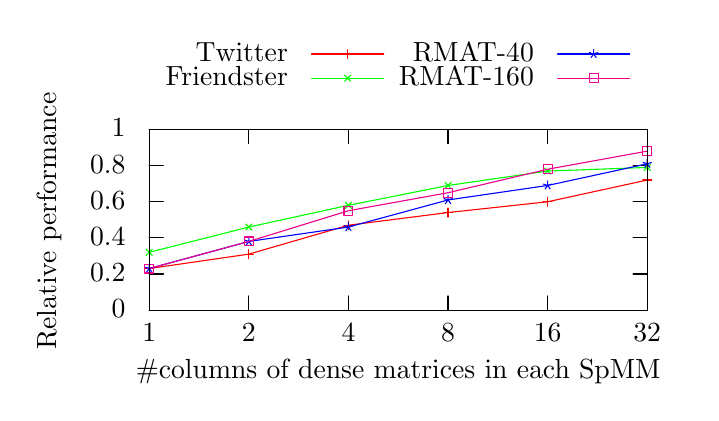
\begin{tikzpicture}[gnuplot]
%% generated with GNUPLOT 4.6p4 (Lua 5.1; terminal rev. 99, script rev. 100)
%% Tue 24 May 2016 11:22:08 AM EDT
\path (0.000,0.000) rectangle (8.382,4.572);
\gpcolor{color=gp lt color border}
\gpsetlinetype{gp lt border}
\gpsetlinewidth{1.00}
\draw[gp path] (1.504,0.985)--(1.684,0.985);
\draw[gp path] (7.829,0.985)--(7.649,0.985);
\node[gp node right] at (1.320,0.985) { 0};
\draw[gp path] (1.504,1.444)--(1.684,1.444);
\draw[gp path] (7.829,1.444)--(7.649,1.444);
\node[gp node right] at (1.320,1.444) { 0.2};
\draw[gp path] (1.504,1.903)--(1.684,1.903);
\draw[gp path] (7.829,1.903)--(7.649,1.903);
\node[gp node right] at (1.320,1.903) { 0.4};
\draw[gp path] (1.504,2.361)--(1.684,2.361);
\draw[gp path] (7.829,2.361)--(7.649,2.361);
\node[gp node right] at (1.320,2.361) { 0.6};
\draw[gp path] (1.504,2.820)--(1.684,2.820);
\draw[gp path] (7.829,2.820)--(7.649,2.820);
\node[gp node right] at (1.320,2.820) { 0.8};
\draw[gp path] (1.504,3.279)--(1.684,3.279);
\draw[gp path] (7.829,3.279)--(7.649,3.279);
\node[gp node right] at (1.320,3.279) { 1};
\draw[gp path] (1.504,0.985)--(1.504,1.165);
\draw[gp path] (1.504,3.279)--(1.504,3.099);
\node[gp node center] at (1.504,0.677) {1};
\draw[gp path] (2.769,0.985)--(2.769,1.165);
\draw[gp path] (2.769,3.279)--(2.769,3.099);
\node[gp node center] at (2.769,0.677) {2};
\draw[gp path] (4.034,0.985)--(4.034,1.165);
\draw[gp path] (4.034,3.279)--(4.034,3.099);
\node[gp node center] at (4.034,0.677) {4};
\draw[gp path] (5.299,0.985)--(5.299,1.165);
\draw[gp path] (5.299,3.279)--(5.299,3.099);
\node[gp node center] at (5.299,0.677) {8};
\draw[gp path] (6.564,0.985)--(6.564,1.165);
\draw[gp path] (6.564,3.279)--(6.564,3.099);
\node[gp node center] at (6.564,0.677) {16};
\draw[gp path] (7.829,0.985)--(7.829,1.165);
\draw[gp path] (7.829,3.279)--(7.829,3.099);
\node[gp node center] at (7.829,0.677) {32};
\draw[gp path] (1.504,3.279)--(1.504,0.985)--(7.829,0.985)--(7.829,3.279)--cycle;
\node[gp node center,rotate=-270] at (0.246,2.132) {Relative performance};
\node[gp node center] at (4.666,0.215) {\#columns of dense matrices in each SpMM};
\node[gp node right] at (3.382,4.238) {Twitter};
\gpcolor{color=gp lt color 0}
\gpsetlinetype{gp lt plot 0}
\draw[gp path] (3.566,4.238)--(4.482,4.238);
\draw[gp path] (1.504,1.513)--(2.769,1.696)--(4.034,2.063)--(5.299,2.224)--(6.564,2.361)%
  --(7.829,2.637);
\gpsetpointsize{4.00}
\gppoint{gp mark 1}{(1.504,1.513)}
\gppoint{gp mark 1}{(2.769,1.696)}
\gppoint{gp mark 1}{(4.034,2.063)}
\gppoint{gp mark 1}{(5.299,2.224)}
\gppoint{gp mark 1}{(6.564,2.361)}
\gppoint{gp mark 1}{(7.829,2.637)}
\gppoint{gp mark 1}{(4.024,4.238)}
\gpcolor{color=gp lt color border}
\node[gp node right] at (3.382,3.930) {Friendster};
\gpcolor{color=gp lt color 1}
\gpsetlinetype{gp lt plot 1}
\draw[gp path] (3.566,3.930)--(4.482,3.930);
\draw[gp path] (1.504,1.719)--(2.769,2.040)--(4.034,2.316)--(5.299,2.568)--(6.564,2.751)%
  --(7.829,2.797);
\gppoint{gp mark 2}{(1.504,1.719)}
\gppoint{gp mark 2}{(2.769,2.040)}
\gppoint{gp mark 2}{(4.034,2.316)}
\gppoint{gp mark 2}{(5.299,2.568)}
\gppoint{gp mark 2}{(6.564,2.751)}
\gppoint{gp mark 2}{(7.829,2.797)}
\gppoint{gp mark 2}{(4.024,3.930)}
\gpcolor{color=gp lt color border}
\node[gp node right] at (6.506,4.238) {RMAT-40};
\gpcolor{color=gp lt color 2}
\gpsetlinetype{gp lt plot 2}
\draw[gp path] (6.690,4.238)--(7.606,4.238);
\draw[gp path] (1.504,1.513)--(2.769,1.857)--(4.034,2.040)--(5.299,2.384)--(6.564,2.568)%
  --(7.829,2.843);
\gppoint{gp mark 3}{(1.504,1.513)}
\gppoint{gp mark 3}{(2.769,1.857)}
\gppoint{gp mark 3}{(4.034,2.040)}
\gppoint{gp mark 3}{(5.299,2.384)}
\gppoint{gp mark 3}{(6.564,2.568)}
\gppoint{gp mark 3}{(7.829,2.843)}
\gppoint{gp mark 3}{(7.148,4.238)}
\gpcolor{color=gp lt color border}
\node[gp node right] at (6.506,3.930) {RMAT-160};
\gpcolor{color=gp lt color 3}
\gpsetlinetype{gp lt plot 3}
\draw[gp path] (6.690,3.930)--(7.606,3.930);
\draw[gp path] (1.504,1.513)--(2.769,1.857)--(4.034,2.247)--(5.299,2.476)--(6.564,2.774)%
  --(7.829,3.004);
\gppoint{gp mark 4}{(1.504,1.513)}
\gppoint{gp mark 4}{(2.769,1.857)}
\gppoint{gp mark 4}{(4.034,2.247)}
\gppoint{gp mark 4}{(5.299,2.476)}
\gppoint{gp mark 4}{(6.564,2.774)}
\gppoint{gp mark 4}{(7.829,3.004)}
\gppoint{gp mark 4}{(7.148,3.930)}
\gpcolor{color=gp lt color border}
\gpsetlinetype{gp lt border}
\draw[gp path] (1.504,3.279)--(1.504,0.985)--(7.829,0.985)--(7.829,3.279)--cycle;
%% coordinates of the plot area
\gpdefrectangularnode{gp plot 1}{\pgfpoint{1.504cm}{0.985cm}}{\pgfpoint{7.829cm}{3.279cm}}
\end{tikzpicture}
%% gnuplot variables

		\caption{The performance of SEM-SpMM with 32-column matrices
			relative to IM-SpMM. SEM-SpMM is broken into multiple SEM-SpMMs
		based on the memory size.}
		\label{perf:spmm32}
	\end{center}
\end{figure}

As more columns in the input dense matrix can fit in memory, the performance
of SEM-SpMM constantly increases (Figure \ref{perf:spmm32}). When the memory
can fit over four columns of the input dense matrix, SEM-SpMM gets over 50\%
of the performance of IM-SpMM. Even when only one column of the input dense
matrix can fit in memory, SEM-SpMM still gets 25\% of the in-memory performance.
When the entire input dense matrix can fit in memory, we get about 80\% of
the in-memory performance.

\begin{figure}
	\begin{center}
		\footnotesize
		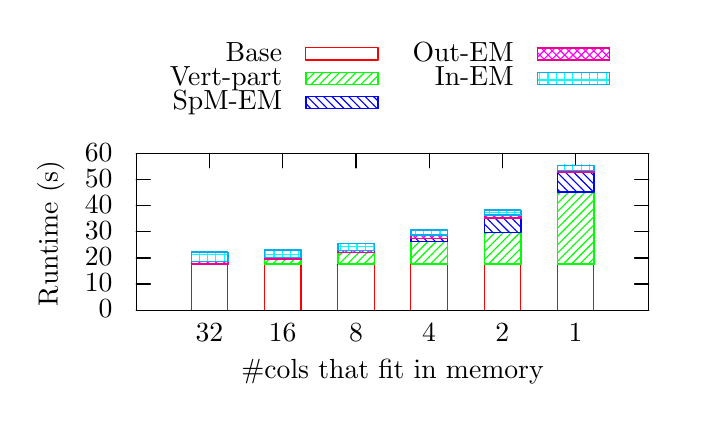
\begin{tikzpicture}[gnuplot]
%% generated with GNUPLOT 4.6p4 (Lua 5.1; terminal rev. 99, script rev. 100)
%% Sun 31 Jan 2016 05:12:26 PM EST
\path (0.000,0.000) rectangle (8.382,4.572);
\gpcolor{color=gp lt color border}
\gpsetlinetype{gp lt border}
\gpsetlinewidth{1.00}
\draw[gp path] (1.320,0.985)--(1.500,0.985);
\draw[gp path] (7.829,0.985)--(7.649,0.985);
\node[gp node right] at (1.136,0.985) { 0};
\draw[gp path] (1.320,1.316)--(1.500,1.316);
\draw[gp path] (7.829,1.316)--(7.649,1.316);
\node[gp node right] at (1.136,1.316) { 10};
\draw[gp path] (1.320,1.647)--(1.500,1.647);
\draw[gp path] (7.829,1.647)--(7.649,1.647);
\node[gp node right] at (1.136,1.647) { 20};
\draw[gp path] (1.320,1.978)--(1.500,1.978);
\draw[gp path] (7.829,1.978)--(7.649,1.978);
\node[gp node right] at (1.136,1.978) { 30};
\draw[gp path] (1.320,2.309)--(1.500,2.309);
\draw[gp path] (7.829,2.309)--(7.649,2.309);
\node[gp node right] at (1.136,2.309) { 40};
\draw[gp path] (1.320,2.640)--(1.500,2.640);
\draw[gp path] (7.829,2.640)--(7.649,2.640);
\node[gp node right] at (1.136,2.640) { 50};
\draw[gp path] (1.320,2.971)--(1.500,2.971);
\draw[gp path] (7.829,2.971)--(7.649,2.971);
\node[gp node right] at (1.136,2.971) { 60};
\draw[gp path] (2.250,0.985)--(2.250,1.165);
\draw[gp path] (2.250,2.971)--(2.250,2.791);
\node[gp node center] at (2.250,0.677) {32};
\draw[gp path] (3.180,0.985)--(3.180,1.165);
\draw[gp path] (3.180,2.971)--(3.180,2.791);
\node[gp node center] at (3.180,0.677) {16};
\draw[gp path] (4.110,0.985)--(4.110,1.165);
\draw[gp path] (4.110,2.971)--(4.110,2.791);
\node[gp node center] at (4.110,0.677) {8};
\draw[gp path] (5.039,0.985)--(5.039,1.165);
\draw[gp path] (5.039,2.971)--(5.039,2.791);
\node[gp node center] at (5.039,0.677) {4};
\draw[gp path] (5.969,0.985)--(5.969,1.165);
\draw[gp path] (5.969,2.971)--(5.969,2.791);
\node[gp node center] at (5.969,0.677) {2};
\draw[gp path] (6.899,0.985)--(6.899,1.165);
\draw[gp path] (6.899,2.971)--(6.899,2.791);
\node[gp node center] at (6.899,0.677) {1};
\draw[gp path] (1.320,2.971)--(1.320,0.985)--(7.829,0.985)--(7.829,2.971)--cycle;
\node[gp node center,rotate=-270] at (0.246,1.978) {Runtime (s)};
\node[gp node center] at (4.574,0.215) {\#cols that fit in memory};
\node[gp node right] at (3.290,4.238) {Base};
\def\gpfillpath{(3.474,4.161)--(4.390,4.161)--(4.390,4.315)--(3.474,4.315)--cycle}
\gpfill{color=gpbgfillcolor} \gpfillpath;
\gpfill{color=gp lt color 0,gp pattern 0,pattern color=.} \gpfillpath;
\gpcolor{color=gp lt color 0}
\gpsetlinetype{gp lt plot 0}
\draw[gp path] (3.474,4.161)--(4.390,4.161)--(4.390,4.315)--(3.474,4.315)--cycle;
\def\gpfillpath{(2.017,0.985)--(2.483,0.985)--(2.483,1.573)--(2.017,1.573)--cycle}
\gpfill{color=gpbgfillcolor} \gpfillpath;
\gpfill{color=gp lt color 0,gp pattern 0,pattern color=.} \gpfillpath;
\draw[gp path] (2.017,0.985)--(2.017,1.572)--(2.482,1.572)--(2.482,0.985)--cycle;
\def\gpfillpath{(2.947,0.985)--(3.413,0.985)--(3.413,1.573)--(2.947,1.573)--cycle}
\gpfill{color=gpbgfillcolor} \gpfillpath;
\gpfill{color=gp lt color 0,gp pattern 0,pattern color=.} \gpfillpath;
\draw[gp path] (2.947,0.985)--(2.947,1.572)--(3.412,1.572)--(3.412,0.985)--cycle;
\def\gpfillpath{(3.877,0.985)--(4.343,0.985)--(4.343,1.573)--(3.877,1.573)--cycle}
\gpfill{color=gpbgfillcolor} \gpfillpath;
\gpfill{color=gp lt color 0,gp pattern 0,pattern color=.} \gpfillpath;
\draw[gp path] (3.877,0.985)--(3.877,1.572)--(4.342,1.572)--(4.342,0.985)--cycle;
\def\gpfillpath{(4.807,0.985)--(5.273,0.985)--(5.273,1.573)--(4.807,1.573)--cycle}
\gpfill{color=gpbgfillcolor} \gpfillpath;
\gpfill{color=gp lt color 0,gp pattern 0,pattern color=.} \gpfillpath;
\draw[gp path] (4.807,0.985)--(4.807,1.572)--(5.272,1.572)--(5.272,0.985)--cycle;
\def\gpfillpath{(5.737,0.985)--(6.203,0.985)--(6.203,1.573)--(5.737,1.573)--cycle}
\gpfill{color=gpbgfillcolor} \gpfillpath;
\gpfill{color=gp lt color 0,gp pattern 0,pattern color=.} \gpfillpath;
\draw[gp path] (5.737,0.985)--(5.737,1.572)--(6.202,1.572)--(6.202,0.985)--cycle;
\def\gpfillpath{(6.667,0.985)--(7.133,0.985)--(7.133,1.573)--(6.667,1.573)--cycle}
\gpfill{color=gpbgfillcolor} \gpfillpath;
\gpfill{color=gp lt color 0,gp pattern 0,pattern color=.} \gpfillpath;
\draw[gp path] (6.667,0.985)--(6.667,1.572)--(7.132,1.572)--(7.132,0.985)--cycle;
\gpcolor{color=gp lt color border}
\node[gp node right] at (3.290,3.930) {Vert-part};
\def\gpfillpath{(3.474,3.853)--(4.390,3.853)--(4.390,4.007)--(3.474,4.007)--cycle}
\gpfill{color=gpbgfillcolor} \gpfillpath;
\gpfill{color=gp lt color 1,gp pattern 1,pattern color=.} \gpfillpath;
\gpcolor{color=gp lt color 1}
\gpsetlinetype{gp lt plot 1}
\draw[gp path] (3.474,3.853)--(4.390,3.853)--(4.390,4.007)--(3.474,4.007)--cycle;
\def\gpfillpath{(2.017,1.572)--(2.483,1.572)--(2.483,1.573)--(2.017,1.573)--cycle}
\gpfill{color=gpbgfillcolor} \gpfillpath;
\gpfill{color=gp lt color 1,gp pattern 1,pattern color=.} \gpfillpath;
\draw[gp path] (2.017,1.572)--(2.482,1.572)--cycle;
\def\gpfillpath{(2.947,1.572)--(3.413,1.572)--(3.413,1.635)--(2.947,1.635)--cycle}
\gpfill{color=gpbgfillcolor} \gpfillpath;
\gpfill{color=gp lt color 1,gp pattern 1,pattern color=.} \gpfillpath;
\draw[gp path] (2.947,1.572)--(2.947,1.634)--(3.412,1.634)--(3.412,1.572)--cycle;
\def\gpfillpath{(3.877,1.572)--(4.343,1.572)--(4.343,1.723)--(3.877,1.723)--cycle}
\gpfill{color=gpbgfillcolor} \gpfillpath;
\gpfill{color=gp lt color 1,gp pattern 1,pattern color=.} \gpfillpath;
\draw[gp path] (3.877,1.572)--(3.877,1.722)--(4.342,1.722)--(4.342,1.572)--cycle;
\def\gpfillpath{(4.807,1.572)--(5.273,1.572)--(5.273,1.859)--(4.807,1.859)--cycle}
\gpfill{color=gpbgfillcolor} \gpfillpath;
\gpfill{color=gp lt color 1,gp pattern 1,pattern color=.} \gpfillpath;
\draw[gp path] (4.807,1.572)--(4.807,1.858)--(5.272,1.858)--(5.272,1.572)--cycle;
\def\gpfillpath{(5.737,1.572)--(6.203,1.572)--(6.203,1.972)--(5.737,1.972)--cycle}
\gpfill{color=gpbgfillcolor} \gpfillpath;
\gpfill{color=gp lt color 1,gp pattern 1,pattern color=.} \gpfillpath;
\draw[gp path] (5.737,1.572)--(5.737,1.971)--(6.202,1.971)--(6.202,1.572)--cycle;
\def\gpfillpath{(6.667,1.572)--(7.133,1.572)--(7.133,2.490)--(6.667,2.490)--cycle}
\gpfill{color=gpbgfillcolor} \gpfillpath;
\gpfill{color=gp lt color 1,gp pattern 1,pattern color=.} \gpfillpath;
\draw[gp path] (6.667,1.572)--(6.667,2.489)--(7.132,2.489)--(7.132,1.572)--cycle;
\gpcolor{color=gp lt color border}
\node[gp node right] at (3.290,3.622) {SpM-EM};
\def\gpfillpath{(3.474,3.545)--(4.390,3.545)--(4.390,3.699)--(3.474,3.699)--cycle}
\gpfill{color=gpbgfillcolor} \gpfillpath;
\gpfill{color=gp lt color 2,gp pattern 2,pattern color=.} \gpfillpath;
\gpcolor{color=gp lt color 2}
\gpsetlinetype{gp lt plot 2}
\draw[gp path] (3.474,3.545)--(4.390,3.545)--(4.390,3.699)--(3.474,3.699)--cycle;
\def\gpfillpath{(2.017,1.572)--(2.483,1.572)--(2.483,1.575)--(2.017,1.575)--cycle}
\gpfill{color=gpbgfillcolor} \gpfillpath;
\gpfill{color=gp lt color 2,gp pattern 2,pattern color=.} \gpfillpath;
\draw[gp path] (2.017,1.572)--(2.017,1.574)--(2.482,1.574)--(2.482,1.572)--cycle;
\def\gpfillpath{(2.947,1.634)--(3.413,1.634)--(3.413,1.635)--(2.947,1.635)--cycle}
\gpfill{color=gpbgfillcolor} \gpfillpath;
\gpfill{color=gp lt color 2,gp pattern 2,pattern color=.} \gpfillpath;
\draw[gp path] (2.947,1.634)--(3.412,1.634)--cycle;
\def\gpfillpath{(3.877,1.722)--(4.343,1.722)--(4.343,1.723)--(3.877,1.723)--cycle}
\gpfill{color=gpbgfillcolor} \gpfillpath;
\gpfill{color=gp lt color 2,gp pattern 2,pattern color=.} \gpfillpath;
\draw[gp path] (3.877,1.722)--(4.342,1.722)--cycle;
\def\gpfillpath{(4.807,1.858)--(5.273,1.858)--(5.273,1.898)--(4.807,1.898)--cycle}
\gpfill{color=gpbgfillcolor} \gpfillpath;
\gpfill{color=gp lt color 2,gp pattern 2,pattern color=.} \gpfillpath;
\draw[gp path] (4.807,1.858)--(4.807,1.897)--(5.272,1.897)--(5.272,1.858)--cycle;
\def\gpfillpath{(5.737,1.971)--(6.203,1.971)--(6.203,2.158)--(5.737,2.158)--cycle}
\gpfill{color=gpbgfillcolor} \gpfillpath;
\gpfill{color=gp lt color 2,gp pattern 2,pattern color=.} \gpfillpath;
\draw[gp path] (5.737,1.971)--(5.737,2.157)--(6.202,2.157)--(6.202,1.971)--cycle;
\def\gpfillpath{(6.667,2.489)--(7.133,2.489)--(7.133,2.740)--(6.667,2.740)--cycle}
\gpfill{color=gpbgfillcolor} \gpfillpath;
\gpfill{color=gp lt color 2,gp pattern 2,pattern color=.} \gpfillpath;
\draw[gp path] (6.667,2.489)--(6.667,2.739)--(7.132,2.739)--(7.132,2.489)--cycle;
\gpcolor{color=gp lt color border}
\node[gp node right] at (6.230,4.238) {Out-EM};
\def\gpfillpath{(6.414,4.161)--(7.330,4.161)--(7.330,4.315)--(6.414,4.315)--cycle}
\gpfill{color=gpbgfillcolor} \gpfillpath;
\gpfill{color=gp lt color 3,gp pattern 3,pattern color=.} \gpfillpath;
\gpcolor{color=gp lt color 3}
\gpsetlinetype{gp lt plot 3}
\draw[gp path] (6.414,4.161)--(7.330,4.161)--(7.330,4.315)--(6.414,4.315)--cycle;
\def\gpfillpath{(2.017,1.574)--(2.483,1.574)--(2.483,1.605)--(2.017,1.605)--cycle}
\gpfill{color=gpbgfillcolor} \gpfillpath;
\gpfill{color=gp lt color 3,gp pattern 3,pattern color=.} \gpfillpath;
\draw[gp path] (2.017,1.574)--(2.017,1.604)--(2.482,1.604)--(2.482,1.574)--cycle;
\def\gpfillpath{(2.947,1.634)--(3.413,1.634)--(3.413,1.655)--(2.947,1.655)--cycle}
\gpfill{color=gpbgfillcolor} \gpfillpath;
\gpfill{color=gp lt color 3,gp pattern 3,pattern color=.} \gpfillpath;
\draw[gp path] (2.947,1.634)--(2.947,1.654)--(3.412,1.654)--(3.412,1.634)--cycle;
\def\gpfillpath{(3.877,1.722)--(4.343,1.722)--(4.343,1.747)--(3.877,1.747)--cycle}
\gpfill{color=gpbgfillcolor} \gpfillpath;
\gpfill{color=gp lt color 3,gp pattern 3,pattern color=.} \gpfillpath;
\draw[gp path] (3.877,1.722)--(3.877,1.746)--(4.342,1.746)--(4.342,1.722)--cycle;
\def\gpfillpath{(4.807,1.897)--(5.273,1.897)--(5.273,1.940)--(4.807,1.940)--cycle}
\gpfill{color=gpbgfillcolor} \gpfillpath;
\gpfill{color=gp lt color 3,gp pattern 3,pattern color=.} \gpfillpath;
\draw[gp path] (4.807,1.897)--(4.807,1.939)--(5.272,1.939)--(5.272,1.897)--cycle;
\def\gpfillpath{(5.737,2.157)--(6.203,2.157)--(6.203,2.195)--(5.737,2.195)--cycle}
\gpfill{color=gpbgfillcolor} \gpfillpath;
\gpfill{color=gp lt color 3,gp pattern 3,pattern color=.} \gpfillpath;
\draw[gp path] (5.737,2.157)--(5.737,2.194)--(6.202,2.194)--(6.202,2.157)--cycle;
\def\gpfillpath{(6.667,2.739)--(7.133,2.739)--(7.133,2.759)--(6.667,2.759)--cycle}
\gpfill{color=gpbgfillcolor} \gpfillpath;
\gpfill{color=gp lt color 3,gp pattern 3,pattern color=.} \gpfillpath;
\draw[gp path] (6.667,2.739)--(6.667,2.758)--(7.132,2.758)--(7.132,2.739)--cycle;
\gpcolor{color=gp lt color border}
\node[gp node right] at (6.230,3.930) {In-EM};
\def\gpfillpath{(6.414,3.853)--(7.330,3.853)--(7.330,4.007)--(6.414,4.007)--cycle}
\gpfill{color=gpbgfillcolor} \gpfillpath;
\gpfill{color=gp lt color 4,gp pattern 4,pattern color=.} \gpfillpath;
\gpcolor{color=gp lt color 4}
\gpsetlinetype{gp lt plot 4}
\draw[gp path] (6.414,3.853)--(7.330,3.853)--(7.330,4.007)--(6.414,4.007)--cycle;
\def\gpfillpath{(2.017,1.604)--(2.483,1.604)--(2.483,1.726)--(2.017,1.726)--cycle}
\gpfill{color=gpbgfillcolor} \gpfillpath;
\gpfill{color=gp lt color 4,gp pattern 4,pattern color=.} \gpfillpath;
\draw[gp path] (2.017,1.604)--(2.017,1.725)--(2.482,1.725)--(2.482,1.604)--cycle;
\def\gpfillpath{(2.947,1.654)--(3.413,1.654)--(3.413,1.752)--(2.947,1.752)--cycle}
\gpfill{color=gpbgfillcolor} \gpfillpath;
\gpfill{color=gp lt color 4,gp pattern 4,pattern color=.} \gpfillpath;
\draw[gp path] (2.947,1.654)--(2.947,1.751)--(3.412,1.751)--(3.412,1.654)--cycle;
\def\gpfillpath{(3.877,1.746)--(4.343,1.746)--(4.343,1.835)--(3.877,1.835)--cycle}
\gpfill{color=gpbgfillcolor} \gpfillpath;
\gpfill{color=gp lt color 4,gp pattern 4,pattern color=.} \gpfillpath;
\draw[gp path] (3.877,1.746)--(3.877,1.834)--(4.342,1.834)--(4.342,1.746)--cycle;
\def\gpfillpath{(4.807,1.939)--(5.273,1.939)--(5.273,2.004)--(4.807,2.004)--cycle}
\gpfill{color=gpbgfillcolor} \gpfillpath;
\gpfill{color=gp lt color 4,gp pattern 4,pattern color=.} \gpfillpath;
\draw[gp path] (4.807,1.939)--(4.807,2.003)--(5.272,2.003)--(5.272,1.939)--cycle;
\def\gpfillpath{(5.737,2.194)--(6.203,2.194)--(6.203,2.259)--(5.737,2.259)--cycle}
\gpfill{color=gpbgfillcolor} \gpfillpath;
\gpfill{color=gp lt color 4,gp pattern 4,pattern color=.} \gpfillpath;
\draw[gp path] (5.737,2.194)--(5.737,2.258)--(6.202,2.258)--(6.202,2.194)--cycle;
\def\gpfillpath{(6.667,2.758)--(7.133,2.758)--(7.133,2.828)--(6.667,2.828)--cycle}
\gpfill{color=gpbgfillcolor} \gpfillpath;
\gpfill{color=gp lt color 4,gp pattern 4,pattern color=.} \gpfillpath;
\draw[gp path] (6.667,2.758)--(6.667,2.827)--(7.132,2.827)--(7.132,2.758)--cycle;
\gpcolor{color=gp lt color border}
\gpsetlinetype{gp lt border}
\draw[gp path] (1.320,2.971)--(1.320,0.985)--(7.829,0.985)--(7.829,2.971)--cycle;
%% coordinates of the plot area
\gpdefrectangularnode{gp plot 1}{\pgfpoint{1.320cm}{0.985cm}}{\pgfpoint{7.829cm}{2.971cm}}
\end{tikzpicture}
%% gnuplot variables

		\caption{The overhead breakdown of SEM-SpMM on the Friendster
			graph with a dense matrix of 32 columns when the number
			of columns that fit in memory varies. }
		\label{perf:spmm32_over}
	\end{center}
\end{figure}

Two main factors lead to performance loss in SEM-SpMM when the input dense matrix
cannot fit in memory. We illustrate the contribution of four potential overheads
in SEM-SpMM on the Friendster graph (Figure \ref{perf:spmm32_over}). The main
performance loss comes from the loss of data locality in SpMM caused by
vertical partitioning of the input dense matrix (Vert-part). Partitioning
the dense matrix into one-column matrices contributes 60\% of performance loss.
It drops quickly when the vertical
partition size increases. Keeping the sparse matrix on SSDs (SpM-EM)
also contributes some performance loss when the dense matrix is partitioned
into small matrices. The overhead almost goes away when more than four columns
of the dense matrix can fit in memory. The overhead of streaming the output dense
matrix to SSDs (Out-EM) and reading the input dense matrix to memory (In-EM)
is less significant and remains the same for different memory sizes.

\subsection{Optimizations on sparse matrix multiplication}
Accelerating SEM-SpMM requires both computation and I/O optimizations.
%Due to the limit of space, we only illustrate the effectiveness of computation
%optimizations.
We first deploy computation optimizations for in-memory sparse matrix
multiplication and then
deploy I/O optimizations for SEM-SpMM with all computation optimizations.

Here we illustrate the most significant optimizations from Section
\ref{sec:spmm}. We start with an in-memory implementation that
performs sparse matrix multiplication on a sparse matrix in the CSR format
and apply the optimizations incrementally in the following order:
\begin{itemize} \itemsep1pt \parskip0pt \parsep0pt
	\item dispatch partitions of a sparse matrix to threads dynamically
		to balance load (\textit{Load balance}),
	\item partition dense matrices for NUMA (\textit{NUMA}),
	\item organize the non-zero entries in a sparse matrix into tiles to
		increase CPU cache hits (\textit{Cache blocking}),
	\item use CPU vectorization instructions to accelerate arithmetic
		computation (\textit{Vec}),
\end{itemize}

All of these optimizations have positive effects on sparse matrix
multiplication and all optimizations together speed up SpMM by $3-5$ times
(Figure \ref{perf:spmm_opt}). The degree of effectiveness
varies between different graphs and different numbers of columns in
the dense matrices. The largest performance boost is from cache blocking,
especially for SpMV.
This is expected because the main overhead of SpMV comes from random memory
access and cache blocking significantly increases CPU cache hits to reduce
random memory access. CPU vectorization is only effective on SpMM because
it optimizes computation on a row of the dense matrix.
%For example, the NUMA optimization is more effective when
%the dense matrices have more columns because more columns in the dense
%matrices require more memory bandwidth. Cache blocking is very effective when
%the dense matrices have fewer columns because it can effectively increase CPU
%cache hits. When there are more columns in the dense matrices, data locality
%improves and the effectiveness of cache blocking becomes less noticeable.
%When there are too many columns, the rows from the input and output matrices
%can no longer be in the CPU cache.
With all optimizations, we have a fast in-memory implementation for both
sparse matrix vector multiplication and sparse matrix dense matrix multiplication.

\begin{figure}
	\begin{center}
		\footnotesize
		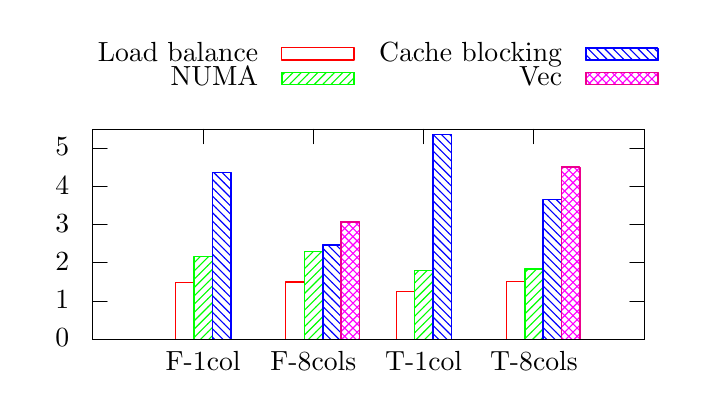
\begin{tikzpicture}[gnuplot]
%% generated with GNUPLOT 4.6p4 (Lua 5.1; terminal rev. 99, script rev. 100)
%% Sat 30 Jan 2016 11:05:37 AM EST
\path (0.000,0.000) rectangle (8.382,4.572);
\gpcolor{color=gp lt color border}
\gpsetlinetype{gp lt border}
\gpsetlinewidth{1.00}
\draw[gp path] (0.828,0.616)--(1.008,0.616);
\draw[gp path] (7.829,0.616)--(7.649,0.616);
\node[gp node right] at (0.644,0.616) { 0};
\draw[gp path] (0.828,1.100)--(1.008,1.100);
\draw[gp path] (7.829,1.100)--(7.649,1.100);
\node[gp node right] at (0.644,1.100) { 1};
\draw[gp path] (0.828,1.584)--(1.008,1.584);
\draw[gp path] (7.829,1.584)--(7.649,1.584);
\node[gp node right] at (0.644,1.584) { 2};
\draw[gp path] (0.828,2.069)--(1.008,2.069);
\draw[gp path] (7.829,2.069)--(7.649,2.069);
\node[gp node right] at (0.644,2.069) { 3};
\draw[gp path] (0.828,2.553)--(1.008,2.553);
\draw[gp path] (7.829,2.553)--(7.649,2.553);
\node[gp node right] at (0.644,2.553) { 4};
\draw[gp path] (0.828,3.037)--(1.008,3.037);
\draw[gp path] (7.829,3.037)--(7.649,3.037);
\node[gp node right] at (0.644,3.037) { 5};
\draw[gp path] (2.228,0.616)--(2.228,0.796);
\draw[gp path] (2.228,3.279)--(2.228,3.099);
\node[gp node center] at (2.228,0.308) {F-1col};
\draw[gp path] (3.628,0.616)--(3.628,0.796);
\draw[gp path] (3.628,3.279)--(3.628,3.099);
\node[gp node center] at (3.628,0.308) {F-8cols};
\draw[gp path] (5.029,0.616)--(5.029,0.796);
\draw[gp path] (5.029,3.279)--(5.029,3.099);
\node[gp node center] at (5.029,0.308) {T-1col};
\draw[gp path] (6.429,0.616)--(6.429,0.796);
\draw[gp path] (6.429,3.279)--(6.429,3.099);
\node[gp node center] at (6.429,0.308) {T-8cols};
\draw[gp path] (0.828,3.279)--(0.828,0.616)--(7.829,0.616)--(7.829,3.279)--cycle;
\node[gp node right] at (3.044,4.238) {Load balance};
\def\gpfillpath{(3.228,4.161)--(4.144,4.161)--(4.144,4.315)--(3.228,4.315)--cycle}
\gpfill{color=gpbgfillcolor} \gpfillpath;
\gpfill{color=gp lt color 0,gp pattern 0,pattern color=.} \gpfillpath;
\gpcolor{color=gp lt color 0}
\gpsetlinetype{gp lt plot 0}
\draw[gp path] (3.228,4.161)--(4.144,4.161)--(4.144,4.315)--(3.228,4.315)--cycle;
\def\gpfillpath{(1.878,0.616)--(2.113,0.616)--(2.113,1.334)--(1.878,1.334)--cycle}
\gpfill{color=gpbgfillcolor} \gpfillpath;
\gpfill{color=gp lt color 0,gp pattern 0,pattern color=.} \gpfillpath;
\draw[gp path] (1.878,0.616)--(1.878,1.333)--(2.112,1.333)--(2.112,0.616)--cycle;
\def\gpfillpath{(3.278,0.616)--(3.513,0.616)--(3.513,1.343)--(3.278,1.343)--cycle}
\gpfill{color=gpbgfillcolor} \gpfillpath;
\gpfill{color=gp lt color 0,gp pattern 0,pattern color=.} \gpfillpath;
\draw[gp path] (3.278,0.616)--(3.278,1.342)--(3.512,1.342)--(3.512,0.616)--cycle;
\def\gpfillpath{(4.679,0.616)--(4.913,0.616)--(4.913,1.222)--(4.679,1.222)--cycle}
\gpfill{color=gpbgfillcolor} \gpfillpath;
\gpfill{color=gp lt color 0,gp pattern 0,pattern color=.} \gpfillpath;
\draw[gp path] (4.679,0.616)--(4.679,1.221)--(4.912,1.221)--(4.912,0.616)--cycle;
\def\gpfillpath{(6.079,0.616)--(6.313,0.616)--(6.313,1.353)--(6.079,1.353)--cycle}
\gpfill{color=gpbgfillcolor} \gpfillpath;
\gpfill{color=gp lt color 0,gp pattern 0,pattern color=.} \gpfillpath;
\draw[gp path] (6.079,0.616)--(6.079,1.352)--(6.312,1.352)--(6.312,0.616)--cycle;
\gpcolor{color=gp lt color border}
\node[gp node right] at (3.044,3.930) {NUMA};
\def\gpfillpath{(3.228,3.853)--(4.144,3.853)--(4.144,4.007)--(3.228,4.007)--cycle}
\gpfill{color=gpbgfillcolor} \gpfillpath;
\gpfill{color=gp lt color 1,gp pattern 1,pattern color=.} \gpfillpath;
\gpcolor{color=gp lt color 1}
\gpsetlinetype{gp lt plot 1}
\draw[gp path] (3.228,3.853)--(4.144,3.853)--(4.144,4.007)--(3.228,4.007)--cycle;
\def\gpfillpath{(2.112,0.616)--(2.346,0.616)--(2.346,1.668)--(2.112,1.668)--cycle}
\gpfill{color=gpbgfillcolor} \gpfillpath;
\gpfill{color=gp lt color 1,gp pattern 1,pattern color=.} \gpfillpath;
\draw[gp path] (2.112,0.616)--(2.112,1.667)--(2.345,1.667)--(2.345,0.616)--cycle;
\def\gpfillpath{(3.512,0.616)--(3.746,0.616)--(3.746,1.731)--(3.512,1.731)--cycle}
\gpfill{color=gpbgfillcolor} \gpfillpath;
\gpfill{color=gp lt color 1,gp pattern 1,pattern color=.} \gpfillpath;
\draw[gp path] (3.512,0.616)--(3.512,1.730)--(3.745,1.730)--(3.745,0.616)--cycle;
\def\gpfillpath{(4.912,0.616)--(5.146,0.616)--(5.146,1.489)--(4.912,1.489)--cycle}
\gpfill{color=gpbgfillcolor} \gpfillpath;
\gpfill{color=gp lt color 1,gp pattern 1,pattern color=.} \gpfillpath;
\draw[gp path] (4.912,0.616)--(4.912,1.488)--(5.145,1.488)--(5.145,0.616)--cycle;
\def\gpfillpath{(6.312,0.616)--(6.546,0.616)--(6.546,1.508)--(6.312,1.508)--cycle}
\gpfill{color=gpbgfillcolor} \gpfillpath;
\gpfill{color=gp lt color 1,gp pattern 1,pattern color=.} \gpfillpath;
\draw[gp path] (6.312,0.616)--(6.312,1.507)--(6.545,1.507)--(6.545,0.616)--cycle;
\gpcolor{color=gp lt color border}
\node[gp node right] at (6.904,4.238) {Cache blocking};
\def\gpfillpath{(7.088,4.161)--(8.004,4.161)--(8.004,4.315)--(7.088,4.315)--cycle}
\gpfill{color=gpbgfillcolor} \gpfillpath;
\gpfill{color=gp lt color 2,gp pattern 2,pattern color=.} \gpfillpath;
\gpcolor{color=gp lt color 2}
\gpsetlinetype{gp lt plot 2}
\draw[gp path] (7.088,4.161)--(8.004,4.161)--(8.004,4.315)--(7.088,4.315)--cycle;
\def\gpfillpath{(2.345,0.616)--(2.579,0.616)--(2.579,2.738)--(2.345,2.738)--cycle}
\gpfill{color=gpbgfillcolor} \gpfillpath;
\gpfill{color=gp lt color 2,gp pattern 2,pattern color=.} \gpfillpath;
\draw[gp path] (2.345,0.616)--(2.345,2.737)--(2.578,2.737)--(2.578,0.616)--cycle;
\def\gpfillpath{(3.745,0.616)--(3.979,0.616)--(3.979,1.813)--(3.745,1.813)--cycle}
\gpfill{color=gpbgfillcolor} \gpfillpath;
\gpfill{color=gp lt color 2,gp pattern 2,pattern color=.} \gpfillpath;
\draw[gp path] (3.745,0.616)--(3.745,1.812)--(3.978,1.812)--(3.978,0.616)--cycle;
\def\gpfillpath{(5.145,0.616)--(5.380,0.616)--(5.380,3.217)--(5.145,3.217)--cycle}
\gpfill{color=gpbgfillcolor} \gpfillpath;
\gpfill{color=gp lt color 2,gp pattern 2,pattern color=.} \gpfillpath;
\draw[gp path] (5.145,0.616)--(5.145,3.216)--(5.379,3.216)--(5.379,0.616)--cycle;
\def\gpfillpath{(6.545,0.616)--(6.780,0.616)--(6.780,2.394)--(6.545,2.394)--cycle}
\gpfill{color=gpbgfillcolor} \gpfillpath;
\gpfill{color=gp lt color 2,gp pattern 2,pattern color=.} \gpfillpath;
\draw[gp path] (6.545,0.616)--(6.545,2.393)--(6.779,2.393)--(6.779,0.616)--cycle;
\gpcolor{color=gp lt color border}
\node[gp node right] at (6.904,3.930) {Vec};
\def\gpfillpath{(7.088,3.853)--(8.004,3.853)--(8.004,4.007)--(7.088,4.007)--cycle}
\gpfill{color=gpbgfillcolor} \gpfillpath;
\gpfill{color=gp lt color 3,gp pattern 3,pattern color=.} \gpfillpath;
\gpcolor{color=gp lt color 3}
\gpsetlinetype{gp lt plot 3}
\draw[gp path] (7.088,3.853)--(8.004,3.853)--(8.004,4.007)--(7.088,4.007)--cycle;
\def\gpfillpath{(3.978,0.616)--(4.213,0.616)--(4.213,2.108)--(3.978,2.108)--cycle}
\gpfill{color=gpbgfillcolor} \gpfillpath;
\gpfill{color=gp lt color 3,gp pattern 3,pattern color=.} \gpfillpath;
\draw[gp path] (3.978,0.616)--(3.978,2.107)--(4.212,2.107)--(4.212,0.616)--cycle;
\def\gpfillpath{(6.779,0.616)--(7.013,0.616)--(7.013,2.806)--(6.779,2.806)--cycle}
\gpfill{color=gpbgfillcolor} \gpfillpath;
\gpfill{color=gp lt color 3,gp pattern 3,pattern color=.} \gpfillpath;
\draw[gp path] (6.779,0.616)--(6.779,2.805)--(7.012,2.805)--(7.012,0.616)--cycle;
\gpcolor{color=gp lt color border}
\gpsetlinetype{gp lt border}
\draw[gp path] (0.828,3.279)--(0.828,0.616)--(7.829,0.616)--(7.829,3.279)--cycle;
%% coordinates of the plot area
\gpdefrectangularnode{gp plot 1}{\pgfpoint{0.828cm}{0.616cm}}{\pgfpoint{7.829cm}{3.279cm}}
\end{tikzpicture}
%% gnuplot variables

		\caption{The speedup of computation optimizations for SpMM on the Friendster
			graph (F) and the Twitter graph (T) for different numbers of
			columns in the dense matrices.}
		\label{perf:spmm_opt}
	\end{center}
\end{figure}

%We implement the base version of SEM-SpMM based on the IM-SpMM implementation
%above. In this implementation, we write the output dense matrix to SSDs.
%SpMM on a dense matrix with a few columns is usually CPU-bound. As such,
%we illustrate the I/O optimizations on the base SEM-SpMV in the following order to show
%their effectiveness:
%\begin{itemize} \itemsep1pt \parskip0pt \parsep0pt
%	\item use a compact sparse matrix format to reduce the number of bits read
%		from SSDs,
%	\item reduce memory allocation overhead with \textit{mmap()} by maintaining
%		a per-thread buffer pool to allocate memory for I/O (\textit{buf pool}),
%	\item reduce the number of thread context switch for I/O access with I/O
%		polling (\textit{polling}),
%	\item order the portions of the output dense matrix globally and stream them
%		to SSDs with large I/O (\textit{global output}).
%\end{itemize}

%\begin{figure}
%	\begin{center}
%		\footnotesize
%		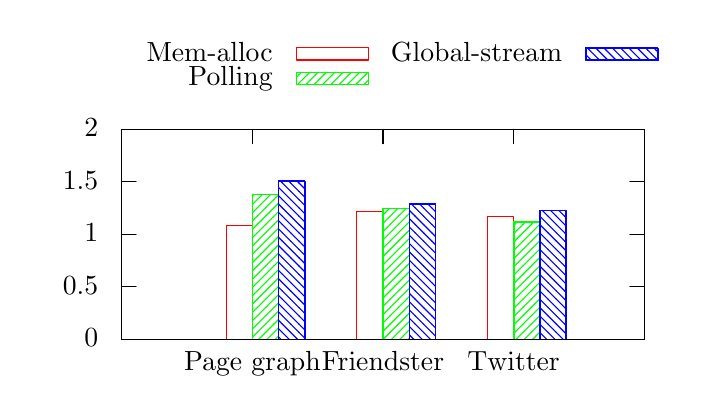
\begin{tikzpicture}[gnuplot]
%% generated with GNUPLOT 4.6p4 (Lua 5.1; terminal rev. 99, script rev. 100)
%% Wed 27 Jan 2016 08:50:42 AM EST
\path (0.000,0.000) rectangle (8.382,4.572);
\gpcolor{color=gp lt color border}
\gpsetlinetype{gp lt border}
\gpsetlinewidth{1.00}
\draw[gp path] (1.196,0.616)--(1.376,0.616);
\draw[gp path] (7.829,0.616)--(7.649,0.616);
\node[gp node right] at (1.012,0.616) { 0};
\draw[gp path] (1.196,1.282)--(1.376,1.282);
\draw[gp path] (7.829,1.282)--(7.649,1.282);
\node[gp node right] at (1.012,1.282) { 0.5};
\draw[gp path] (1.196,1.948)--(1.376,1.948);
\draw[gp path] (7.829,1.948)--(7.649,1.948);
\node[gp node right] at (1.012,1.948) { 1};
\draw[gp path] (1.196,2.613)--(1.376,2.613);
\draw[gp path] (7.829,2.613)--(7.649,2.613);
\node[gp node right] at (1.012,2.613) { 1.5};
\draw[gp path] (1.196,3.279)--(1.376,3.279);
\draw[gp path] (7.829,3.279)--(7.649,3.279);
\node[gp node right] at (1.012,3.279) { 2};
\draw[gp path] (2.854,0.616)--(2.854,0.796);
\draw[gp path] (2.854,3.279)--(2.854,3.099);
\node[gp node center] at (2.854,0.308) {Page graph};
\draw[gp path] (4.513,0.616)--(4.513,0.796);
\draw[gp path] (4.513,3.279)--(4.513,3.099);
\node[gp node center] at (4.513,0.308) {Friendster};
\draw[gp path] (6.171,0.616)--(6.171,0.796);
\draw[gp path] (6.171,3.279)--(6.171,3.099);
\node[gp node center] at (6.171,0.308) {Twitter};
\draw[gp path] (1.196,3.279)--(1.196,0.616)--(7.829,0.616)--(7.829,3.279)--cycle;
\node[gp node right] at (3.228,4.238) {Mem-alloc};
\def\gpfillpath{(3.412,4.161)--(4.328,4.161)--(4.328,4.315)--(3.412,4.315)--cycle}
\gpfill{color=gpbgfillcolor} \gpfillpath;
\gpfill{color=gp lt color 0,gp pattern 0,pattern color=.} \gpfillpath;
\gpcolor{color=gp lt color 0}
\gpsetlinetype{gp lt plot 0}
\draw[gp path] (3.412,4.161)--(4.328,4.161)--(4.328,4.315)--(3.412,4.315)--cycle;
\def\gpfillpath{(2.523,0.616)--(2.855,0.616)--(2.855,2.055)--(2.523,2.055)--cycle}
\gpfill{color=gpbgfillcolor} \gpfillpath;
\gpfill{color=gp lt color 0,gp pattern 0,pattern color=.} \gpfillpath;
\draw[gp path] (2.523,0.616)--(2.523,2.054)--(2.854,2.054)--(2.854,0.616)--cycle;
\def\gpfillpath{(4.181,0.616)--(4.514,0.616)--(4.514,2.241)--(4.181,2.241)--cycle}
\gpfill{color=gpbgfillcolor} \gpfillpath;
\gpfill{color=gp lt color 0,gp pattern 0,pattern color=.} \gpfillpath;
\draw[gp path] (4.181,0.616)--(4.181,2.240)--(4.513,2.240)--(4.513,0.616)--cycle;
\def\gpfillpath{(5.839,0.616)--(6.172,0.616)--(6.172,2.175)--(5.839,2.175)--cycle}
\gpfill{color=gpbgfillcolor} \gpfillpath;
\gpfill{color=gp lt color 0,gp pattern 0,pattern color=.} \gpfillpath;
\draw[gp path] (5.839,0.616)--(5.839,2.174)--(6.171,2.174)--(6.171,0.616)--cycle;
\gpcolor{color=gp lt color border}
\node[gp node right] at (3.228,3.930) {Polling};
\def\gpfillpath{(3.412,3.853)--(4.328,3.853)--(4.328,4.007)--(3.412,4.007)--cycle}
\gpfill{color=gpbgfillcolor} \gpfillpath;
\gpfill{color=gp lt color 1,gp pattern 1,pattern color=.} \gpfillpath;
\gpcolor{color=gp lt color 1}
\gpsetlinetype{gp lt plot 1}
\draw[gp path] (3.412,3.853)--(4.328,3.853)--(4.328,4.007)--(3.412,4.007)--cycle;
\def\gpfillpath{(2.854,0.616)--(3.187,0.616)--(3.187,2.454)--(2.854,2.454)--cycle}
\gpfill{color=gpbgfillcolor} \gpfillpath;
\gpfill{color=gp lt color 1,gp pattern 1,pattern color=.} \gpfillpath;
\draw[gp path] (2.854,0.616)--(2.854,2.453)--(3.186,2.453)--(3.186,0.616)--cycle;
\def\gpfillpath{(4.513,0.616)--(4.845,0.616)--(4.845,2.281)--(4.513,2.281)--cycle}
\gpfill{color=gpbgfillcolor} \gpfillpath;
\gpfill{color=gp lt color 1,gp pattern 1,pattern color=.} \gpfillpath;
\draw[gp path] (4.513,0.616)--(4.513,2.280)--(4.844,2.280)--(4.844,0.616)--cycle;
\def\gpfillpath{(6.171,0.616)--(6.503,0.616)--(6.503,2.108)--(6.171,2.108)--cycle}
\gpfill{color=gpbgfillcolor} \gpfillpath;
\gpfill{color=gp lt color 1,gp pattern 1,pattern color=.} \gpfillpath;
\draw[gp path] (6.171,0.616)--(6.171,2.107)--(6.502,2.107)--(6.502,0.616)--cycle;
\gpcolor{color=gp lt color border}
\node[gp node right] at (6.904,4.238) {Global-stream};
\def\gpfillpath{(7.088,4.161)--(8.004,4.161)--(8.004,4.315)--(7.088,4.315)--cycle}
\gpfill{color=gpbgfillcolor} \gpfillpath;
\gpfill{color=gp lt color 2,gp pattern 2,pattern color=.} \gpfillpath;
\gpcolor{color=gp lt color 2}
\gpsetlinetype{gp lt plot 2}
\draw[gp path] (7.088,4.161)--(8.004,4.161)--(8.004,4.315)--(7.088,4.315)--cycle;
\def\gpfillpath{(3.186,0.616)--(3.519,0.616)--(3.519,2.628)--(3.186,2.628)--cycle}
\gpfill{color=gpbgfillcolor} \gpfillpath;
\gpfill{color=gp lt color 2,gp pattern 2,pattern color=.} \gpfillpath;
\draw[gp path] (3.186,0.616)--(3.186,2.627)--(3.518,2.627)--(3.518,0.616)--cycle;
\def\gpfillpath{(4.844,0.616)--(5.177,0.616)--(5.177,2.335)--(4.844,2.335)--cycle}
\gpfill{color=gpbgfillcolor} \gpfillpath;
\gpfill{color=gp lt color 2,gp pattern 2,pattern color=.} \gpfillpath;
\draw[gp path] (4.844,0.616)--(4.844,2.334)--(5.176,2.334)--(5.176,0.616)--cycle;
\def\gpfillpath{(6.502,0.616)--(6.835,0.616)--(6.835,2.255)--(6.502,2.255)--cycle}
\gpfill{color=gpbgfillcolor} \gpfillpath;
\gpfill{color=gp lt color 2,gp pattern 2,pattern color=.} \gpfillpath;
\draw[gp path] (6.502,0.616)--(6.502,2.254)--(6.834,2.254)--(6.834,0.616)--cycle;
\gpcolor{color=gp lt color border}
\gpsetlinetype{gp lt border}
\draw[gp path] (1.196,3.279)--(1.196,0.616)--(7.829,0.616)--(7.829,3.279)--cycle;
%% coordinates of the plot area
\gpdefrectangularnode{gp plot 1}{\pgfpoint{1.196cm}{0.616cm}}{\pgfpoint{7.829cm}{3.279cm}}
\end{tikzpicture}
%% gnuplot variables

%		\caption{The speedup of I/O optimizations for SpMV on real-world graphs.}
%		\label{perf:spmm_opt_io}
%	\end{center}
%\end{figure}

%SEM-SpMV on some of the graphs requires substantial I/O throughput and
%any improvement on I/O leads to overall performance boost (Figure
%\ref{perf:spmm_opt_io}). The Page graph is relatively well clustered, so
%SEM-SpMV on this graph is less computationally intensive than other graphs
%and requires higher I/O throughput.
%Using a compact sparse matrix format accelerates the information retrieval
%of the sparse matrix and gives us the best performance boost among all
%optimizations. Reducing the overhead of memory allocation with \textit{mmap()}
%gives significant performance boost. Reducing the number of thread context
%switches with polling achieve substantial performance improvement. 

\subsection{Performance of the applications}

We evaluate the performance of our implementations of the applications in
Section \ref{sec:apps}. We show the effectiveness of additional memory for
these applications and compare their performance with state-of-the-art
implementations on smaller graphs.

\subsubsection{PageRank}
We evaluate the performance of our SpMM-based PageRank implementation
(SpMM-PageRank). This implementation requires the input vector to be in memory,
but it is optional to keep the output vector and the degree vector in memory.
PageRank is a benchmarking graph algorithm implemented by many graph processing
frameworks. We compare the performance of SpMM-PageRank with state-of-the-art
implementations in FlashGraph \cite{flashgraph}, a semi-external memory graph
engine, and GraphLab Create, the next generation of PowerGraph \cite{powergraph}.
The PageRank implementation in FlashGraph computes
approximate PageRank values while SpMM-PageRank and GraphLab Create compute
exact PageRank values. We run GraphLab Create completely in memory and
FlashGraph in semi-external memory. GraphLab Create is not able to compute
PageRank on the Page graph. We use FlashGraph v0.3 and a trial version of
GraphLab Create v1.9.

SpMM-PageRank in memory and in semi-external memory both significantly outperforms
the implementations in FlashGraph and GraphLab Create (Figure \ref{perf:pagerank})
even though FlashGraph computes approximate PageRank and GraphLab Create runs
completely in memory. The main computation of PageRank is to access PageRank
values from neighbor vertices, which is essentially the same computation in
sparse matrix vector multiplication. Our SpMM is highly optimized for both CPU
and I/O. Even though SpMM-PageRank performs more computation than FlashGraph,
it performs the computation much more efficiently and
reads less data from SSDs than FlashGraph. SpMM-PageRank and the implementation
in GraphLab create performs the same computation, but SpMM-PageRank
performs the computation much more efficiently.

The experiment results also show that keeping more vectors in memory has modest
performance improvement for SpMM-PageRank. As such, SpMM-PageRank only needs
to keep one vector in memory, which results in very small memory consumption.

\begin{figure}
	\begin{center}
		\footnotesize
		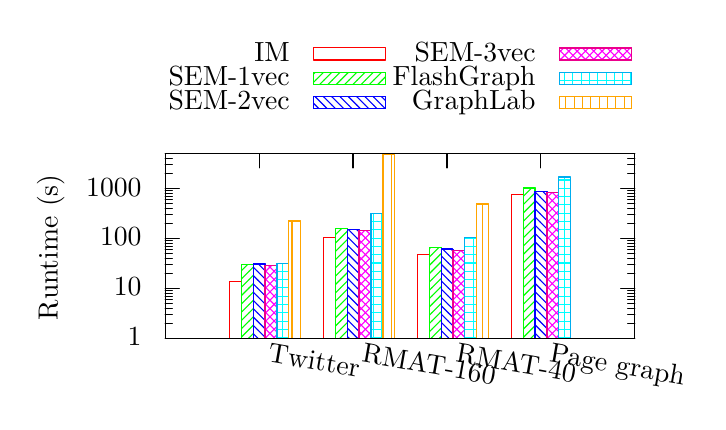
\begin{tikzpicture}[gnuplot]
%% generated with GNUPLOT 4.6p4 (Lua 5.1; terminal rev. 99, script rev. 100)
%% Wed 20 Jan 2016 10:17:41 PM EST
\path (0.000,0.000) rectangle (8.382,4.572);
\gpcolor{color=gp lt color border}
\gpsetlinetype{gp lt border}
\gpsetlinewidth{1.00}
\draw[gp path] (1.688,0.627)--(1.868,0.627);
\draw[gp path] (7.651,0.627)--(7.471,0.627);
\node[gp node right] at (1.504,0.627) { 1};
\draw[gp path] (1.688,0.818)--(1.778,0.818);
\draw[gp path] (7.651,0.818)--(7.561,0.818);
\draw[gp path] (1.688,0.929)--(1.778,0.929);
\draw[gp path] (7.651,0.929)--(7.561,0.929);
\draw[gp path] (1.688,1.009)--(1.778,1.009);
\draw[gp path] (7.651,1.009)--(7.561,1.009);
\draw[gp path] (1.688,1.070)--(1.778,1.070);
\draw[gp path] (7.651,1.070)--(7.561,1.070);
\draw[gp path] (1.688,1.120)--(1.778,1.120);
\draw[gp path] (7.651,1.120)--(7.561,1.120);
\draw[gp path] (1.688,1.163)--(1.778,1.163);
\draw[gp path] (7.651,1.163)--(7.561,1.163);
\draw[gp path] (1.688,1.199)--(1.778,1.199);
\draw[gp path] (7.651,1.199)--(7.561,1.199);
\draw[gp path] (1.688,1.232)--(1.778,1.232);
\draw[gp path] (7.651,1.232)--(7.561,1.232);
\draw[gp path] (1.688,1.261)--(1.868,1.261);
\draw[gp path] (7.651,1.261)--(7.471,1.261);
\node[gp node right] at (1.504,1.261) { 10};
\draw[gp path] (1.688,1.451)--(1.778,1.451);
\draw[gp path] (7.651,1.451)--(7.561,1.451);
\draw[gp path] (1.688,1.563)--(1.778,1.563);
\draw[gp path] (7.651,1.563)--(7.561,1.563);
\draw[gp path] (1.688,1.642)--(1.778,1.642);
\draw[gp path] (7.651,1.642)--(7.561,1.642);
\draw[gp path] (1.688,1.704)--(1.778,1.704);
\draw[gp path] (7.651,1.704)--(7.561,1.704);
\draw[gp path] (1.688,1.754)--(1.778,1.754);
\draw[gp path] (7.651,1.754)--(7.561,1.754);
\draw[gp path] (1.688,1.796)--(1.778,1.796);
\draw[gp path] (7.651,1.796)--(7.561,1.796);
\draw[gp path] (1.688,1.833)--(1.778,1.833);
\draw[gp path] (7.651,1.833)--(7.561,1.833);
\draw[gp path] (1.688,1.865)--(1.778,1.865);
\draw[gp path] (7.651,1.865)--(7.561,1.865);
\draw[gp path] (1.688,1.894)--(1.868,1.894);
\draw[gp path] (7.651,1.894)--(7.471,1.894);
\node[gp node right] at (1.504,1.894) { 100};
\draw[gp path] (1.688,2.085)--(1.778,2.085);
\draw[gp path] (7.651,2.085)--(7.561,2.085);
\draw[gp path] (1.688,2.197)--(1.778,2.197);
\draw[gp path] (7.651,2.197)--(7.561,2.197);
\draw[gp path] (1.688,2.276)--(1.778,2.276);
\draw[gp path] (7.651,2.276)--(7.561,2.276);
\draw[gp path] (1.688,2.337)--(1.778,2.337);
\draw[gp path] (7.651,2.337)--(7.561,2.337);
\draw[gp path] (1.688,2.387)--(1.778,2.387);
\draw[gp path] (7.651,2.387)--(7.561,2.387);
\draw[gp path] (1.688,2.430)--(1.778,2.430);
\draw[gp path] (7.651,2.430)--(7.561,2.430);
\draw[gp path] (1.688,2.467)--(1.778,2.467);
\draw[gp path] (7.651,2.467)--(7.561,2.467);
\draw[gp path] (1.688,2.499)--(1.778,2.499);
\draw[gp path] (7.651,2.499)--(7.561,2.499);
\draw[gp path] (1.688,2.528)--(1.868,2.528);
\draw[gp path] (7.651,2.528)--(7.471,2.528);
\node[gp node right] at (1.504,2.528) { 1000};
\draw[gp path] (1.688,2.719)--(1.778,2.719);
\draw[gp path] (7.651,2.719)--(7.561,2.719);
\draw[gp path] (1.688,2.830)--(1.778,2.830);
\draw[gp path] (7.651,2.830)--(7.561,2.830);
\draw[gp path] (1.688,2.910)--(1.778,2.910);
\draw[gp path] (7.651,2.910)--(7.561,2.910);
\draw[gp path] (1.688,2.971)--(1.778,2.971);
\draw[gp path] (7.651,2.971)--(7.561,2.971);
\draw[gp path] (2.881,0.627)--(2.881,0.807);
\draw[gp path] (2.881,2.971)--(2.881,2.791);
\node[gp node left,rotate=-10] at (2.881,0.443) {Twitter};
\draw[gp path] (4.073,0.627)--(4.073,0.807);
\draw[gp path] (4.073,2.971)--(4.073,2.791);
\node[gp node left,rotate=-10] at (4.073,0.443) {RMAT-160};
\draw[gp path] (5.266,0.627)--(5.266,0.807);
\draw[gp path] (5.266,2.971)--(5.266,2.791);
\node[gp node left,rotate=-10] at (5.266,0.443) {RMAT-40};
\draw[gp path] (6.458,0.627)--(6.458,0.807);
\draw[gp path] (6.458,2.971)--(6.458,2.791);
\node[gp node left,rotate=-10] at (6.458,0.443) {Page graph};
\draw[gp path] (1.688,2.971)--(1.688,0.627)--(7.651,0.627)--(7.651,2.971)--cycle;
\node[gp node center,rotate=-270] at (0.246,1.799) {Runtime (s)};
\node[gp node right] at (3.385,4.238) {IM};
\def\gpfillpath{(3.569,4.161)--(4.485,4.161)--(4.485,4.315)--(3.569,4.315)--cycle}
\gpfill{color=gpbgfillcolor} \gpfillpath;
\gpfill{color=gp lt color 0,gp pattern 0,pattern color=.} \gpfillpath;
\gpcolor{color=gp lt color 0}
\gpsetlinetype{gp lt plot 0}
\draw[gp path] (3.569,4.161)--(4.485,4.161)--(4.485,4.315)--(3.569,4.315)--cycle;
\def\gpfillpath{(2.508,0.627)--(2.658,0.627)--(2.658,1.346)--(2.508,1.346)--cycle}
\gpfill{color=gpbgfillcolor} \gpfillpath;
\gpfill{color=gp lt color 0,gp pattern 0,pattern color=.} \gpfillpath;
\draw[gp path] (2.508,0.627)--(2.508,1.345)--(2.657,1.345)--(2.657,0.627)--cycle;
\def\gpfillpath{(3.701,0.627)--(3.851,0.627)--(3.851,1.912)--(3.701,1.912)--cycle}
\gpfill{color=gpbgfillcolor} \gpfillpath;
\gpfill{color=gp lt color 0,gp pattern 0,pattern color=.} \gpfillpath;
\draw[gp path] (3.701,0.627)--(3.701,1.911)--(3.850,1.911)--(3.850,0.627)--cycle;
\def\gpfillpath{(4.893,0.627)--(5.043,0.627)--(5.043,1.692)--(4.893,1.692)--cycle}
\gpfill{color=gpbgfillcolor} \gpfillpath;
\gpfill{color=gp lt color 0,gp pattern 0,pattern color=.} \gpfillpath;
\draw[gp path] (4.893,0.627)--(4.893,1.691)--(5.042,1.691)--(5.042,0.627)--cycle;
\def\gpfillpath{(6.086,0.627)--(6.236,0.627)--(6.236,2.452)--(6.086,2.452)--cycle}
\gpfill{color=gpbgfillcolor} \gpfillpath;
\gpfill{color=gp lt color 0,gp pattern 0,pattern color=.} \gpfillpath;
\draw[gp path] (6.086,0.627)--(6.086,2.451)--(6.235,2.451)--(6.235,0.627)--cycle;
\gpcolor{color=gp lt color border}
\node[gp node right] at (3.385,3.930) {SEM-1vec};
\def\gpfillpath{(3.569,3.853)--(4.485,3.853)--(4.485,4.007)--(3.569,4.007)--cycle}
\gpfill{color=gpbgfillcolor} \gpfillpath;
\gpfill{color=gp lt color 1,gp pattern 1,pattern color=.} \gpfillpath;
\gpcolor{color=gp lt color 1}
\gpsetlinetype{gp lt plot 1}
\draw[gp path] (3.569,3.853)--(4.485,3.853)--(4.485,4.007)--(3.569,4.007)--cycle;
\def\gpfillpath{(2.657,0.627)--(2.807,0.627)--(2.807,1.567)--(2.657,1.567)--cycle}
\gpfill{color=gpbgfillcolor} \gpfillpath;
\gpfill{color=gp lt color 1,gp pattern 1,pattern color=.} \gpfillpath;
\draw[gp path] (2.657,0.627)--(2.657,1.566)--(2.806,1.566)--(2.806,0.627)--cycle;
\def\gpfillpath{(3.850,0.627)--(4.000,0.627)--(4.000,2.024)--(3.850,2.024)--cycle}
\gpfill{color=gpbgfillcolor} \gpfillpath;
\gpfill{color=gp lt color 1,gp pattern 1,pattern color=.} \gpfillpath;
\draw[gp path] (3.850,0.627)--(3.850,2.023)--(3.999,2.023)--(3.999,0.627)--cycle;
\def\gpfillpath{(5.042,0.627)--(5.192,0.627)--(5.192,1.782)--(5.042,1.782)--cycle}
\gpfill{color=gpbgfillcolor} \gpfillpath;
\gpfill{color=gp lt color 1,gp pattern 1,pattern color=.} \gpfillpath;
\draw[gp path] (5.042,0.627)--(5.042,1.781)--(5.191,1.781)--(5.191,0.627)--cycle;
\def\gpfillpath{(6.235,0.627)--(6.385,0.627)--(6.385,2.539)--(6.235,2.539)--cycle}
\gpfill{color=gpbgfillcolor} \gpfillpath;
\gpfill{color=gp lt color 1,gp pattern 1,pattern color=.} \gpfillpath;
\draw[gp path] (6.235,0.627)--(6.235,2.538)--(6.384,2.538)--(6.384,0.627)--cycle;
\gpcolor{color=gp lt color border}
\node[gp node right] at (3.385,3.622) {SEM-2vec};
\def\gpfillpath{(3.569,3.545)--(4.485,3.545)--(4.485,3.699)--(3.569,3.699)--cycle}
\gpfill{color=gpbgfillcolor} \gpfillpath;
\gpfill{color=gp lt color 2,gp pattern 2,pattern color=.} \gpfillpath;
\gpcolor{color=gp lt color 2}
\gpsetlinetype{gp lt plot 2}
\draw[gp path] (3.569,3.545)--(4.485,3.545)--(4.485,3.699)--(3.569,3.699)--cycle;
\def\gpfillpath{(2.806,0.627)--(2.956,0.627)--(2.956,1.576)--(2.806,1.576)--cycle}
\gpfill{color=gpbgfillcolor} \gpfillpath;
\gpfill{color=gp lt color 2,gp pattern 2,pattern color=.} \gpfillpath;
\draw[gp path] (2.806,0.627)--(2.806,1.575)--(2.955,1.575)--(2.955,0.627)--cycle;
\def\gpfillpath{(3.999,0.627)--(4.149,0.627)--(4.149,2.013)--(3.999,2.013)--cycle}
\gpfill{color=gpbgfillcolor} \gpfillpath;
\gpfill{color=gp lt color 2,gp pattern 2,pattern color=.} \gpfillpath;
\draw[gp path] (3.999,0.627)--(3.999,2.012)--(4.148,2.012)--(4.148,0.627)--cycle;
\def\gpfillpath{(5.191,0.627)--(5.341,0.627)--(5.341,1.764)--(5.191,1.764)--cycle}
\gpfill{color=gpbgfillcolor} \gpfillpath;
\gpfill{color=gp lt color 2,gp pattern 2,pattern color=.} \gpfillpath;
\draw[gp path] (5.191,0.627)--(5.191,1.763)--(5.340,1.763)--(5.340,0.627)--cycle;
\def\gpfillpath{(6.384,0.627)--(6.534,0.627)--(6.534,2.493)--(6.384,2.493)--cycle}
\gpfill{color=gpbgfillcolor} \gpfillpath;
\gpfill{color=gp lt color 2,gp pattern 2,pattern color=.} \gpfillpath;
\draw[gp path] (6.384,0.627)--(6.384,2.492)--(6.533,2.492)--(6.533,0.627)--cycle;
\gpcolor{color=gp lt color border}
\node[gp node right] at (6.509,4.238) {SEM-3vec};
\def\gpfillpath{(6.693,4.161)--(7.609,4.161)--(7.609,4.315)--(6.693,4.315)--cycle}
\gpfill{color=gpbgfillcolor} \gpfillpath;
\gpfill{color=gp lt color 3,gp pattern 3,pattern color=.} \gpfillpath;
\gpcolor{color=gp lt color 3}
\gpsetlinetype{gp lt plot 3}
\draw[gp path] (6.693,4.161)--(7.609,4.161)--(7.609,4.315)--(6.693,4.315)--cycle;
\def\gpfillpath{(2.955,0.627)--(3.105,0.627)--(3.105,1.555)--(2.955,1.555)--cycle}
\gpfill{color=gpbgfillcolor} \gpfillpath;
\gpfill{color=gp lt color 3,gp pattern 3,pattern color=.} \gpfillpath;
\draw[gp path] (2.955,0.627)--(2.955,1.554)--(3.104,1.554)--(3.104,0.627)--cycle;
\def\gpfillpath{(4.148,0.627)--(4.298,0.627)--(4.298,2.002)--(4.148,2.002)--cycle}
\gpfill{color=gpbgfillcolor} \gpfillpath;
\gpfill{color=gp lt color 3,gp pattern 3,pattern color=.} \gpfillpath;
\draw[gp path] (4.148,0.627)--(4.148,2.001)--(4.297,2.001)--(4.297,0.627)--cycle;
\def\gpfillpath{(5.340,0.627)--(5.490,0.627)--(5.490,1.742)--(5.340,1.742)--cycle}
\gpfill{color=gpbgfillcolor} \gpfillpath;
\gpfill{color=gp lt color 3,gp pattern 3,pattern color=.} \gpfillpath;
\draw[gp path] (5.340,0.627)--(5.340,1.741)--(5.489,1.741)--(5.489,0.627)--cycle;
\def\gpfillpath{(6.533,0.627)--(6.683,0.627)--(6.683,2.484)--(6.533,2.484)--cycle}
\gpfill{color=gpbgfillcolor} \gpfillpath;
\gpfill{color=gp lt color 3,gp pattern 3,pattern color=.} \gpfillpath;
\draw[gp path] (6.533,0.627)--(6.533,2.483)--(6.682,2.483)--(6.682,0.627)--cycle;
\gpcolor{color=gp lt color border}
\node[gp node right] at (6.509,3.930) {FlashGraph};
\def\gpfillpath{(6.693,3.853)--(7.609,3.853)--(7.609,4.007)--(6.693,4.007)--cycle}
\gpfill{color=gpbgfillcolor} \gpfillpath;
\gpfill{color=gp lt color 4,gp pattern 4,pattern color=.} \gpfillpath;
\gpcolor{color=gp lt color 4}
\gpsetlinetype{gp lt plot 4}
\draw[gp path] (6.693,3.853)--(7.609,3.853)--(7.609,4.007)--(6.693,4.007)--cycle;
\def\gpfillpath{(3.104,0.627)--(3.254,0.627)--(3.254,1.581)--(3.104,1.581)--cycle}
\gpfill{color=gpbgfillcolor} \gpfillpath;
\gpfill{color=gp lt color 4,gp pattern 4,pattern color=.} \gpfillpath;
\draw[gp path] (3.104,0.627)--(3.104,1.580)--(3.253,1.580)--(3.253,0.627)--cycle;
\def\gpfillpath{(4.297,0.627)--(4.447,0.627)--(4.447,2.218)--(4.297,2.218)--cycle}
\gpfill{color=gpbgfillcolor} \gpfillpath;
\gpfill{color=gp lt color 4,gp pattern 4,pattern color=.} \gpfillpath;
\draw[gp path] (4.297,0.627)--(4.297,2.217)--(4.446,2.217)--(4.446,0.627)--cycle;
\def\gpfillpath{(5.489,0.627)--(5.639,0.627)--(5.639,1.907)--(5.489,1.907)--cycle}
\gpfill{color=gpbgfillcolor} \gpfillpath;
\gpfill{color=gp lt color 4,gp pattern 4,pattern color=.} \gpfillpath;
\draw[gp path] (5.489,0.627)--(5.489,1.906)--(5.638,1.906)--(5.638,0.627)--cycle;
\def\gpfillpath{(6.682,0.627)--(6.832,0.627)--(6.832,2.677)--(6.682,2.677)--cycle}
\gpfill{color=gpbgfillcolor} \gpfillpath;
\gpfill{color=gp lt color 4,gp pattern 4,pattern color=.} \gpfillpath;
\draw[gp path] (6.682,0.627)--(6.682,2.676)--(6.831,2.676)--(6.831,0.627)--cycle;
\gpcolor{color=gp lt color border}
\node[gp node right] at (6.509,3.622) {GraphLab};
\def\gpfillpath{(6.693,3.545)--(7.609,3.545)--(7.609,3.699)--(6.693,3.699)--cycle}
\gpfill{color=gpbgfillcolor} \gpfillpath;
\gpfill{rgb color={1.000,0.647,0.000},gp pattern 5,pattern color=.} \gpfillpath;
\gpcolor{rgb color={1.000,0.647,0.000}}
\gpsetlinetype{gp lt plot 5}
\draw[gp path] (6.693,3.545)--(7.609,3.545)--(7.609,3.699)--(6.693,3.699)--cycle;
\def\gpfillpath{(3.253,0.627)--(3.403,0.627)--(3.403,2.119)--(3.253,2.119)--cycle}
\gpfill{color=gpbgfillcolor} \gpfillpath;
\gpfill{rgb color={1.000,0.647,0.000},gp pattern 5,pattern color=.} \gpfillpath;
\draw[gp path] (3.253,0.627)--(3.253,2.118)--(3.402,2.118)--(3.402,0.627)--cycle;
\def\gpfillpath{(4.446,0.627)--(4.596,0.627)--(4.596,2.970)--(4.446,2.970)--cycle}
\gpfill{color=gpbgfillcolor} \gpfillpath;
\gpfill{rgb color={1.000,0.647,0.000},gp pattern 5,pattern color=.} \gpfillpath;
\draw[gp path] (4.446,0.627)--(4.446,2.969)--(4.595,2.969)--(4.595,0.627)--cycle;
\def\gpfillpath{(5.638,0.627)--(5.789,0.627)--(5.789,2.337)--(5.638,2.337)--cycle}
\gpfill{color=gpbgfillcolor} \gpfillpath;
\gpfill{rgb color={1.000,0.647,0.000},gp pattern 5,pattern color=.} \gpfillpath;
\draw[gp path] (5.638,0.627)--(5.638,2.336)--(5.788,2.336)--(5.788,0.627)--cycle;
\gpcolor{color=gp lt color border}
\gpsetlinetype{gp lt border}
\draw[gp path] (1.688,2.971)--(1.688,0.627)--(7.651,0.627)--(7.651,2.971)--cycle;
%% coordinates of the plot area
\gpdefrectangularnode{gp plot 1}{\pgfpoint{1.688cm}{0.627cm}}{\pgfpoint{7.651cm}{2.971cm}}
\end{tikzpicture}
%% gnuplot variables

		\caption{The runtime of SpMM-PageRank in 30 iterations. The SEM
			implementation keeps different numbers of vectors in memory.
			We compare them with the implementations in FlashGraph and GraphLab
		Create.}
		\label{perf:pagerank}
	\end{center}
\end{figure}

\subsubsection{Eigensolver}

We evaluate the performance of our SEM KrylovSchur eigensolver and compare
its performance
with our in-memory eigensolver and the Trilinos KrylovSchur eigensolver.
Usually, spectral analysis only requires a very small number of
eigenvalues, so we compute eight eigenvalues in this experiment. We run
the eigensolvers on the smaller undirected graphs
in Table \ref{graphs}. To evaluate the scalability of the SEM eigensolver,
we compute singular value decomposition (SVD) on the Page graph. Among all of
the eigensolvers, only our SEM eigensolver is able to compute eigenvalues
on the Page graph.

\begin{figure}
	\begin{center}
		\footnotesize
		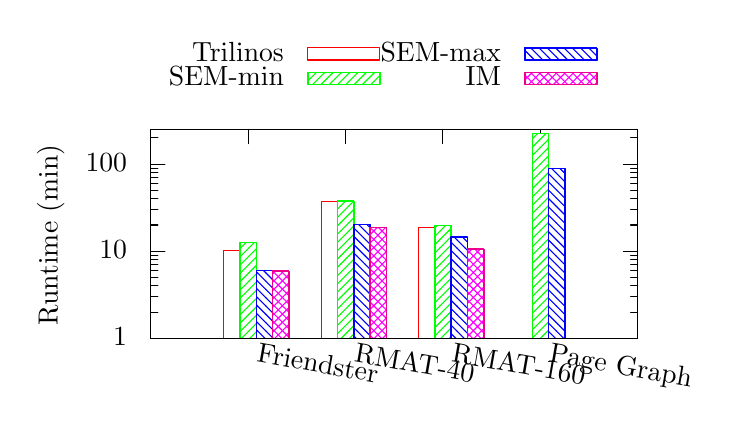
\begin{tikzpicture}[gnuplot]
%% generated with GNUPLOT 4.6p4 (Lua 5.1; terminal rev. 99, script rev. 100)
%% Mon 01 Feb 2016 08:09:35 PM EST
\path (0.000,0.000) rectangle (8.382,4.572);
\gpcolor{color=gp lt color border}
\gpsetlinetype{gp lt border}
\gpsetlinewidth{1.00}
\draw[gp path] (1.504,0.627)--(1.684,0.627);
\draw[gp path] (7.688,0.627)--(7.508,0.627);
\node[gp node right] at (1.320,0.627) { 1};
\draw[gp path] (1.504,0.960)--(1.594,0.960);
\draw[gp path] (7.688,0.960)--(7.598,0.960);
\draw[gp path] (1.504,1.155)--(1.594,1.155);
\draw[gp path] (7.688,1.155)--(7.598,1.155);
\draw[gp path] (1.504,1.293)--(1.594,1.293);
\draw[gp path] (7.688,1.293)--(7.598,1.293);
\draw[gp path] (1.504,1.400)--(1.594,1.400);
\draw[gp path] (7.688,1.400)--(7.598,1.400);
\draw[gp path] (1.504,1.488)--(1.594,1.488);
\draw[gp path] (7.688,1.488)--(7.598,1.488);
\draw[gp path] (1.504,1.562)--(1.594,1.562);
\draw[gp path] (7.688,1.562)--(7.598,1.562);
\draw[gp path] (1.504,1.626)--(1.594,1.626);
\draw[gp path] (7.688,1.626)--(7.598,1.626);
\draw[gp path] (1.504,1.682)--(1.594,1.682);
\draw[gp path] (7.688,1.682)--(7.598,1.682);
\draw[gp path] (1.504,1.733)--(1.684,1.733);
\draw[gp path] (7.688,1.733)--(7.508,1.733);
\node[gp node right] at (1.320,1.733) { 10};
\draw[gp path] (1.504,2.066)--(1.594,2.066);
\draw[gp path] (7.688,2.066)--(7.598,2.066);
\draw[gp path] (1.504,2.261)--(1.594,2.261);
\draw[gp path] (7.688,2.261)--(7.598,2.261);
\draw[gp path] (1.504,2.399)--(1.594,2.399);
\draw[gp path] (7.688,2.399)--(7.598,2.399);
\draw[gp path] (1.504,2.506)--(1.594,2.506);
\draw[gp path] (7.688,2.506)--(7.598,2.506);
\draw[gp path] (1.504,2.594)--(1.594,2.594);
\draw[gp path] (7.688,2.594)--(7.598,2.594);
\draw[gp path] (1.504,2.668)--(1.594,2.668);
\draw[gp path] (7.688,2.668)--(7.598,2.668);
\draw[gp path] (1.504,2.732)--(1.594,2.732);
\draw[gp path] (7.688,2.732)--(7.598,2.732);
\draw[gp path] (1.504,2.788)--(1.594,2.788);
\draw[gp path] (7.688,2.788)--(7.598,2.788);
\draw[gp path] (1.504,2.839)--(1.684,2.839);
\draw[gp path] (7.688,2.839)--(7.508,2.839);
\node[gp node right] at (1.320,2.839) { 100};
\draw[gp path] (1.504,3.172)--(1.594,3.172);
\draw[gp path] (7.688,3.172)--(7.598,3.172);
\draw[gp path] (2.741,0.627)--(2.741,0.807);
\draw[gp path] (2.741,3.279)--(2.741,3.099);
\node[gp node left,rotate=-10] at (2.741,0.443) {Friendster};
\draw[gp path] (3.978,0.627)--(3.978,0.807);
\draw[gp path] (3.978,3.279)--(3.978,3.099);
\node[gp node left,rotate=-10] at (3.978,0.443) {RMAT-40};
\draw[gp path] (5.214,0.627)--(5.214,0.807);
\draw[gp path] (5.214,3.279)--(5.214,3.099);
\node[gp node left,rotate=-10] at (5.214,0.443) {RMAT-160};
\draw[gp path] (6.451,0.627)--(6.451,0.807);
\draw[gp path] (6.451,3.279)--(6.451,3.099);
\node[gp node left,rotate=-10] at (6.451,0.443) {Page Graph};
\draw[gp path] (1.504,3.279)--(1.504,0.627)--(7.688,0.627)--(7.688,3.279)--cycle;
\node[gp node center,rotate=-270] at (0.246,1.953) {Runtime (min)};
\node[gp node right] at (3.312,4.238) {Trilinos};
\def\gpfillpath{(3.496,4.161)--(4.412,4.161)--(4.412,4.315)--(3.496,4.315)--cycle}
\gpfill{color=gpbgfillcolor} \gpfillpath;
\gpfill{color=gp lt color 0,gp pattern 0,pattern color=.} \gpfillpath;
\gpcolor{color=gp lt color 0}
\gpsetlinetype{gp lt plot 0}
\draw[gp path] (3.496,4.161)--(4.412,4.161)--(4.412,4.315)--(3.496,4.315)--cycle;
\def\gpfillpath{(2.432,0.627)--(2.639,0.627)--(2.639,1.739)--(2.432,1.739)--cycle}
\gpfill{color=gpbgfillcolor} \gpfillpath;
\gpfill{color=gp lt color 0,gp pattern 0,pattern color=.} \gpfillpath;
\draw[gp path] (2.432,0.627)--(2.432,1.738)--(2.638,1.738)--(2.638,0.627)--cycle;
\def\gpfillpath{(3.668,0.627)--(3.876,0.627)--(3.876,2.360)--(3.668,2.360)--cycle}
\gpfill{color=gpbgfillcolor} \gpfillpath;
\gpfill{color=gp lt color 0,gp pattern 0,pattern color=.} \gpfillpath;
\draw[gp path] (3.668,0.627)--(3.668,2.359)--(3.875,2.359)--(3.875,0.627)--cycle;
\def\gpfillpath{(4.905,0.627)--(5.112,0.627)--(5.112,2.032)--(4.905,2.032)--cycle}
\gpfill{color=gpbgfillcolor} \gpfillpath;
\gpfill{color=gp lt color 0,gp pattern 0,pattern color=.} \gpfillpath;
\draw[gp path] (4.905,0.627)--(4.905,2.031)--(5.111,2.031)--(5.111,0.627)--cycle;
\gpcolor{color=gp lt color border}
\node[gp node right] at (3.312,3.930) {SEM-min};
\def\gpfillpath{(3.496,3.853)--(4.412,3.853)--(4.412,4.007)--(3.496,4.007)--cycle}
\gpfill{color=gpbgfillcolor} \gpfillpath;
\gpfill{color=gp lt color 1,gp pattern 1,pattern color=.} \gpfillpath;
\gpcolor{color=gp lt color 1}
\gpsetlinetype{gp lt plot 1}
\draw[gp path] (3.496,3.853)--(4.412,3.853)--(4.412,4.007)--(3.496,4.007)--cycle;
\def\gpfillpath{(2.638,0.627)--(2.845,0.627)--(2.845,1.846)--(2.638,1.846)--cycle}
\gpfill{color=gpbgfillcolor} \gpfillpath;
\gpfill{color=gp lt color 1,gp pattern 1,pattern color=.} \gpfillpath;
\draw[gp path] (2.638,0.627)--(2.638,1.845)--(2.844,1.845)--(2.844,0.627)--cycle;
\def\gpfillpath{(3.875,0.627)--(4.082,0.627)--(4.082,2.375)--(3.875,2.375)--cycle}
\gpfill{color=gpbgfillcolor} \gpfillpath;
\gpfill{color=gp lt color 1,gp pattern 1,pattern color=.} \gpfillpath;
\draw[gp path] (3.875,0.627)--(3.875,2.374)--(4.081,2.374)--(4.081,0.627)--cycle;
\def\gpfillpath{(5.111,0.627)--(5.318,0.627)--(5.318,2.064)--(5.111,2.064)--cycle}
\gpfill{color=gpbgfillcolor} \gpfillpath;
\gpfill{color=gp lt color 1,gp pattern 1,pattern color=.} \gpfillpath;
\draw[gp path] (5.111,0.627)--(5.111,2.063)--(5.317,2.063)--(5.317,0.627)--cycle;
\def\gpfillpath{(6.348,0.627)--(6.555,0.627)--(6.555,3.229)--(6.348,3.229)--cycle}
\gpfill{color=gpbgfillcolor} \gpfillpath;
\gpfill{color=gp lt color 1,gp pattern 1,pattern color=.} \gpfillpath;
\draw[gp path] (6.348,0.627)--(6.348,3.228)--(6.554,3.228)--(6.554,0.627)--cycle;
\gpcolor{color=gp lt color border}
\node[gp node right] at (6.068,4.238) {SEM-max};
\def\gpfillpath{(6.252,4.161)--(7.168,4.161)--(7.168,4.315)--(6.252,4.315)--cycle}
\gpfill{color=gpbgfillcolor} \gpfillpath;
\gpfill{color=gp lt color 2,gp pattern 2,pattern color=.} \gpfillpath;
\gpcolor{color=gp lt color 2}
\gpsetlinetype{gp lt plot 2}
\draw[gp path] (6.252,4.161)--(7.168,4.161)--(7.168,4.315)--(6.252,4.315)--cycle;
\def\gpfillpath{(2.844,0.627)--(3.051,0.627)--(3.051,1.491)--(2.844,1.491)--cycle}
\gpfill{color=gpbgfillcolor} \gpfillpath;
\gpfill{color=gp lt color 2,gp pattern 2,pattern color=.} \gpfillpath;
\draw[gp path] (2.844,0.627)--(2.844,1.490)--(3.050,1.490)--(3.050,0.627)--cycle;
\def\gpfillpath{(4.081,0.627)--(4.288,0.627)--(4.288,2.077)--(4.081,2.077)--cycle}
\gpfill{color=gpbgfillcolor} \gpfillpath;
\gpfill{color=gp lt color 2,gp pattern 2,pattern color=.} \gpfillpath;
\draw[gp path] (4.081,0.627)--(4.081,2.076)--(4.287,2.076)--(4.287,0.627)--cycle;
\def\gpfillpath{(5.317,0.627)--(5.525,0.627)--(5.525,1.915)--(5.317,1.915)--cycle}
\gpfill{color=gpbgfillcolor} \gpfillpath;
\gpfill{color=gp lt color 2,gp pattern 2,pattern color=.} \gpfillpath;
\draw[gp path] (5.317,0.627)--(5.317,1.914)--(5.524,1.914)--(5.524,0.627)--cycle;
\def\gpfillpath{(6.554,0.627)--(6.761,0.627)--(6.761,2.784)--(6.554,2.784)--cycle}
\gpfill{color=gpbgfillcolor} \gpfillpath;
\gpfill{color=gp lt color 2,gp pattern 2,pattern color=.} \gpfillpath;
\draw[gp path] (6.554,0.627)--(6.554,2.783)--(6.760,2.783)--(6.760,0.627)--cycle;
\gpcolor{color=gp lt color border}
\node[gp node right] at (6.068,3.930) {IM};
\def\gpfillpath{(6.252,3.853)--(7.168,3.853)--(7.168,4.007)--(6.252,4.007)--cycle}
\gpfill{color=gpbgfillcolor} \gpfillpath;
\gpfill{color=gp lt color 3,gp pattern 3,pattern color=.} \gpfillpath;
\gpcolor{color=gp lt color 3}
\gpsetlinetype{gp lt plot 3}
\draw[gp path] (6.252,3.853)--(7.168,3.853)--(7.168,4.007)--(6.252,4.007)--cycle;
\def\gpfillpath{(3.050,0.627)--(3.257,0.627)--(3.257,1.487)--(3.050,1.487)--cycle}
\gpfill{color=gpbgfillcolor} \gpfillpath;
\gpfill{color=gp lt color 3,gp pattern 3,pattern color=.} \gpfillpath;
\draw[gp path] (3.050,0.627)--(3.050,1.486)--(3.256,1.486)--(3.256,0.627)--cycle;
\def\gpfillpath{(4.287,0.627)--(4.494,0.627)--(4.494,2.037)--(4.287,2.037)--cycle}
\gpfill{color=gpbgfillcolor} \gpfillpath;
\gpfill{color=gp lt color 3,gp pattern 3,pattern color=.} \gpfillpath;
\draw[gp path] (4.287,0.627)--(4.287,2.036)--(4.493,2.036)--(4.493,0.627)--cycle;
\def\gpfillpath{(5.524,0.627)--(5.731,0.627)--(5.731,1.762)--(5.524,1.762)--cycle}
\gpfill{color=gpbgfillcolor} \gpfillpath;
\gpfill{color=gp lt color 3,gp pattern 3,pattern color=.} \gpfillpath;
\draw[gp path] (5.524,0.627)--(5.524,1.761)--(5.730,1.761)--(5.730,0.627)--cycle;
\gpcolor{color=gp lt color border}
\gpsetlinetype{gp lt border}
\draw[gp path] (1.504,3.279)--(1.504,0.627)--(7.688,0.627)--(7.688,3.279)--cycle;
%% coordinates of the plot area
\gpdefrectangularnode{gp plot 1}{\pgfpoint{1.504cm}{0.627cm}}{\pgfpoint{7.688cm}{3.279cm}}
\end{tikzpicture}
%% gnuplot variables

		\caption{The performance of our SEM KrylovSchur, our in-memory eigensolver
			and the Trilinos eigensolvers when computing eight
			eigenvalues. SEM-min keeps the entire vector subspace on SSDs and
		SEM-max keeps the entire vector subspace in memory.}
		\label{fig:eigen}
	\end{center}
\end{figure}

For computing 8 eigenvalues, our SEM eigensolver achieves performance
comparable to our in-memory eigensolver and the Trilinos eigensolver
and can scale to very large graphs (Figure \ref{fig:eigen}).
Unlike PageRank, an eigensolver has many more vector or dense matrix operations.
As such, the memory size has noticeable impact on performance.
For the setting with the minimum memory consumption, it has at least 45\%
performance of our in-memory eigensolver; when keeping the entire subspace
in memory, it has almost the same performance as our in-memory eigensolver.

\subsubsection{NMF}
We evaluate the performance of our NMF implementation (SEM-NMF) on the directed
graphs in Table \ref{graphs}. The dense matrices for NMF can be as large as
the sparse matrix. As such, we experiment with the effect of the memory size on
the performance of SEM-NMF by varying the number of columns in memory from
the dense matrices. We also compare the performance of SEM-NMF with
a high-performance NMF implementation SmallK \cite{SmallK}, built on top of
the numeric library Elemental \cite{elemental}. We factorize
each of the graphs into two $n \times k$ non-negative dense matrices and
we use $k=16$ because $16$ is the largest $k$ that SmallK supports for
the graphs in Table \ref{graphs}. We use SmallK v1.6 and Elemental v0.85.

\begin{figure}
	\begin{center}
		\footnotesize
		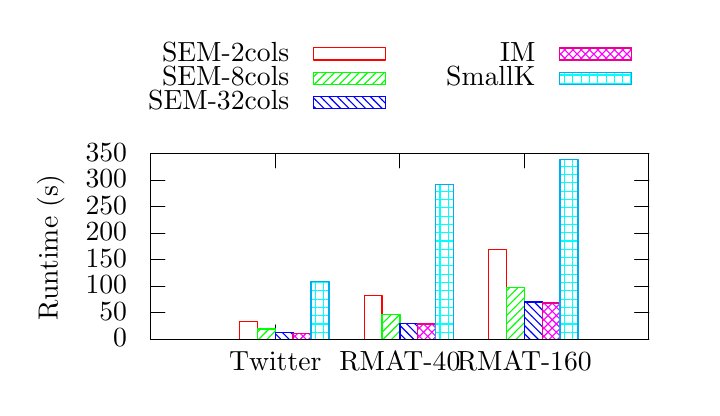
\begin{tikzpicture}[gnuplot]
%% generated with GNUPLOT 4.6p4 (Lua 5.1; terminal rev. 99, script rev. 100)
%% Thu 04 Feb 2016 04:38:14 PM EST
\path (0.000,0.000) rectangle (8.382,4.572);
\gpcolor{color=gp lt color border}
\gpsetlinetype{gp lt border}
\gpsetlinewidth{1.00}
\draw[gp path] (1.504,0.616)--(1.684,0.616);
\draw[gp path] (7.829,0.616)--(7.649,0.616);
\node[gp node right] at (1.320,0.616) { 0};
\draw[gp path] (1.504,0.952)--(1.684,0.952);
\draw[gp path] (7.829,0.952)--(7.649,0.952);
\node[gp node right] at (1.320,0.952) { 50};
\draw[gp path] (1.504,1.289)--(1.684,1.289);
\draw[gp path] (7.829,1.289)--(7.649,1.289);
\node[gp node right] at (1.320,1.289) { 100};
\draw[gp path] (1.504,1.625)--(1.684,1.625);
\draw[gp path] (7.829,1.625)--(7.649,1.625);
\node[gp node right] at (1.320,1.625) { 150};
\draw[gp path] (1.504,1.962)--(1.684,1.962);
\draw[gp path] (7.829,1.962)--(7.649,1.962);
\node[gp node right] at (1.320,1.962) { 200};
\draw[gp path] (1.504,2.298)--(1.684,2.298);
\draw[gp path] (7.829,2.298)--(7.649,2.298);
\node[gp node right] at (1.320,2.298) { 250};
\draw[gp path] (1.504,2.635)--(1.684,2.635);
\draw[gp path] (7.829,2.635)--(7.649,2.635);
\node[gp node right] at (1.320,2.635) { 300};
\draw[gp path] (1.504,2.971)--(1.684,2.971);
\draw[gp path] (7.829,2.971)--(7.649,2.971);
\node[gp node right] at (1.320,2.971) { 350};
\draw[gp path] (3.085,0.616)--(3.085,0.796);
\draw[gp path] (3.085,2.971)--(3.085,2.791);
\node[gp node center] at (3.085,0.308) {Twitter};
\draw[gp path] (4.667,0.616)--(4.667,0.796);
\draw[gp path] (4.667,2.971)--(4.667,2.791);
\node[gp node center] at (4.667,0.308) {RMAT-40};
\draw[gp path] (6.248,0.616)--(6.248,0.796);
\draw[gp path] (6.248,2.971)--(6.248,2.791);
\node[gp node center] at (6.248,0.308) {RMAT-160};
\draw[gp path] (1.504,2.971)--(1.504,0.616)--(7.829,0.616)--(7.829,2.971)--cycle;
\node[gp node center,rotate=-270] at (0.246,1.793) {Runtime (s)};
\node[gp node right] at (3.382,4.238) {SEM-2cols};
\def\gpfillpath{(3.566,4.161)--(4.482,4.161)--(4.482,4.315)--(3.566,4.315)--cycle}
\gpfill{color=gpbgfillcolor} \gpfillpath;
\gpfill{color=gp lt color 0,gp pattern 0,pattern color=.} \gpfillpath;
\gpcolor{color=gp lt color 0}
\gpsetlinetype{gp lt plot 0}
\draw[gp path] (3.566,4.161)--(4.482,4.161)--(4.482,4.315)--(3.566,4.315)--cycle;
\def\gpfillpath{(2.633,0.616)--(2.860,0.616)--(2.860,0.843)--(2.633,0.843)--cycle}
\gpfill{color=gpbgfillcolor} \gpfillpath;
\gpfill{color=gp lt color 0,gp pattern 0,pattern color=.} \gpfillpath;
\draw[gp path] (2.633,0.616)--(2.633,0.842)--(2.859,0.842)--(2.859,0.616)--cycle;
\def\gpfillpath{(4.215,0.616)--(4.442,0.616)--(4.442,1.166)--(4.215,1.166)--cycle}
\gpfill{color=gpbgfillcolor} \gpfillpath;
\gpfill{color=gp lt color 0,gp pattern 0,pattern color=.} \gpfillpath;
\draw[gp path] (4.215,0.616)--(4.215,1.165)--(4.441,1.165)--(4.441,0.616)--cycle;
\def\gpfillpath{(5.796,0.616)--(6.023,0.616)--(6.023,1.751)--(5.796,1.751)--cycle}
\gpfill{color=gpbgfillcolor} \gpfillpath;
\gpfill{color=gp lt color 0,gp pattern 0,pattern color=.} \gpfillpath;
\draw[gp path] (5.796,0.616)--(5.796,1.750)--(6.022,1.750)--(6.022,0.616)--cycle;
\gpcolor{color=gp lt color border}
\node[gp node right] at (3.382,3.930) {SEM-8cols};
\def\gpfillpath{(3.566,3.853)--(4.482,3.853)--(4.482,4.007)--(3.566,4.007)--cycle}
\gpfill{color=gpbgfillcolor} \gpfillpath;
\gpfill{color=gp lt color 1,gp pattern 1,pattern color=.} \gpfillpath;
\gpcolor{color=gp lt color 1}
\gpsetlinetype{gp lt plot 1}
\draw[gp path] (3.566,3.853)--(4.482,3.853)--(4.482,4.007)--(3.566,4.007)--cycle;
\def\gpfillpath{(2.859,0.616)--(3.086,0.616)--(3.086,0.746)--(2.859,0.746)--cycle}
\gpfill{color=gpbgfillcolor} \gpfillpath;
\gpfill{color=gp lt color 1,gp pattern 1,pattern color=.} \gpfillpath;
\draw[gp path] (2.859,0.616)--(2.859,0.745)--(3.085,0.745)--(3.085,0.616)--cycle;
\def\gpfillpath{(4.441,0.616)--(4.668,0.616)--(4.668,0.931)--(4.441,0.931)--cycle}
\gpfill{color=gpbgfillcolor} \gpfillpath;
\gpfill{color=gp lt color 1,gp pattern 1,pattern color=.} \gpfillpath;
\draw[gp path] (4.441,0.616)--(4.441,0.930)--(4.667,0.930)--(4.667,0.616)--cycle;
\def\gpfillpath{(6.022,0.616)--(6.249,0.616)--(6.249,1.274)--(6.022,1.274)--cycle}
\gpfill{color=gpbgfillcolor} \gpfillpath;
\gpfill{color=gp lt color 1,gp pattern 1,pattern color=.} \gpfillpath;
\draw[gp path] (6.022,0.616)--(6.022,1.273)--(6.248,1.273)--(6.248,0.616)--cycle;
\gpcolor{color=gp lt color border}
\node[gp node right] at (3.382,3.622) {SEM-32cols};
\def\gpfillpath{(3.566,3.545)--(4.482,3.545)--(4.482,3.699)--(3.566,3.699)--cycle}
\gpfill{color=gpbgfillcolor} \gpfillpath;
\gpfill{color=gp lt color 2,gp pattern 2,pattern color=.} \gpfillpath;
\gpcolor{color=gp lt color 2}
\gpsetlinetype{gp lt plot 2}
\draw[gp path] (3.566,3.545)--(4.482,3.545)--(4.482,3.699)--(3.566,3.699)--cycle;
\def\gpfillpath{(3.085,0.616)--(3.312,0.616)--(3.312,0.701)--(3.085,0.701)--cycle}
\gpfill{color=gpbgfillcolor} \gpfillpath;
\gpfill{color=gp lt color 2,gp pattern 2,pattern color=.} \gpfillpath;
\draw[gp path] (3.085,0.616)--(3.085,0.700)--(3.311,0.700)--(3.311,0.616)--cycle;
\def\gpfillpath{(4.667,0.616)--(4.893,0.616)--(4.893,0.818)--(4.667,0.818)--cycle}
\gpfill{color=gpbgfillcolor} \gpfillpath;
\gpfill{color=gp lt color 2,gp pattern 2,pattern color=.} \gpfillpath;
\draw[gp path] (4.667,0.616)--(4.667,0.817)--(4.892,0.817)--(4.892,0.616)--cycle;
\def\gpfillpath{(6.248,0.616)--(6.475,0.616)--(6.475,1.093)--(6.248,1.093)--cycle}
\gpfill{color=gpbgfillcolor} \gpfillpath;
\gpfill{color=gp lt color 2,gp pattern 2,pattern color=.} \gpfillpath;
\draw[gp path] (6.248,0.616)--(6.248,1.092)--(6.474,1.092)--(6.474,0.616)--cycle;
\gpcolor{color=gp lt color border}
\node[gp node right] at (6.506,4.238) {IM};
\def\gpfillpath{(6.690,4.161)--(7.606,4.161)--(7.606,4.315)--(6.690,4.315)--cycle}
\gpfill{color=gpbgfillcolor} \gpfillpath;
\gpfill{color=gp lt color 3,gp pattern 3,pattern color=.} \gpfillpath;
\gpcolor{color=gp lt color 3}
\gpsetlinetype{gp lt plot 3}
\draw[gp path] (6.690,4.161)--(7.606,4.161)--(7.606,4.315)--(6.690,4.315)--cycle;
\def\gpfillpath{(3.311,0.616)--(3.538,0.616)--(3.538,0.691)--(3.311,0.691)--cycle}
\gpfill{color=gpbgfillcolor} \gpfillpath;
\gpfill{color=gp lt color 3,gp pattern 3,pattern color=.} \gpfillpath;
\draw[gp path] (3.311,0.616)--(3.311,0.690)--(3.537,0.690)--(3.537,0.616)--cycle;
\def\gpfillpath{(4.892,0.616)--(5.119,0.616)--(5.119,0.809)--(4.892,0.809)--cycle}
\gpfill{color=gpbgfillcolor} \gpfillpath;
\gpfill{color=gp lt color 3,gp pattern 3,pattern color=.} \gpfillpath;
\draw[gp path] (4.892,0.616)--(4.892,0.808)--(5.118,0.808)--(5.118,0.616)--cycle;
\def\gpfillpath{(6.474,0.616)--(6.701,0.616)--(6.701,1.077)--(6.474,1.077)--cycle}
\gpfill{color=gpbgfillcolor} \gpfillpath;
\gpfill{color=gp lt color 3,gp pattern 3,pattern color=.} \gpfillpath;
\draw[gp path] (6.474,0.616)--(6.474,1.076)--(6.700,1.076)--(6.700,0.616)--cycle;
\gpcolor{color=gp lt color border}
\node[gp node right] at (6.506,3.930) {SmallK};
\def\gpfillpath{(6.690,3.853)--(7.606,3.853)--(7.606,4.007)--(6.690,4.007)--cycle}
\gpfill{color=gpbgfillcolor} \gpfillpath;
\gpfill{color=gp lt color 4,gp pattern 4,pattern color=.} \gpfillpath;
\gpcolor{color=gp lt color 4}
\gpsetlinetype{gp lt plot 4}
\draw[gp path] (6.690,3.853)--(7.606,3.853)--(7.606,4.007)--(6.690,4.007)--cycle;
\def\gpfillpath{(3.537,0.616)--(3.764,0.616)--(3.764,1.353)--(3.537,1.353)--cycle}
\gpfill{color=gpbgfillcolor} \gpfillpath;
\gpfill{color=gp lt color 4,gp pattern 4,pattern color=.} \gpfillpath;
\draw[gp path] (3.537,0.616)--(3.537,1.352)--(3.763,1.352)--(3.763,0.616)--cycle;
\def\gpfillpath{(5.118,0.616)--(5.345,0.616)--(5.345,2.582)--(5.118,2.582)--cycle}
\gpfill{color=gpbgfillcolor} \gpfillpath;
\gpfill{color=gp lt color 4,gp pattern 4,pattern color=.} \gpfillpath;
\draw[gp path] (5.118,0.616)--(5.118,2.581)--(5.344,2.581)--(5.344,0.616)--cycle;
\def\gpfillpath{(6.700,0.616)--(6.926,0.616)--(6.926,2.903)--(6.700,2.903)--cycle}
\gpfill{color=gpbgfillcolor} \gpfillpath;
\gpfill{color=gp lt color 4,gp pattern 4,pattern color=.} \gpfillpath;
\draw[gp path] (6.700,0.616)--(6.700,2.902)--(6.925,2.902)--(6.925,0.616)--cycle;
\gpcolor{color=gp lt color border}
\gpsetlinetype{gp lt border}
\draw[gp path] (1.504,2.971)--(1.504,0.616)--(7.829,0.616)--(7.829,2.971)--cycle;
%% coordinates of the plot area
\gpdefrectangularnode{gp plot 1}{\pgfpoint{1.504cm}{0.616cm}}{\pgfpoint{7.829cm}{2.971cm}}
\end{tikzpicture}
%% gnuplot variables

		\caption{The runtime per iteration of SEM-NMF on directed graphs.
			We vary the number of columns in the dense matrices that are kept
			in memory to evaluate effect of the memory size on the performance
		of SEM-NMF.}
		\label{perf:NMF}
	\end{center}
\end{figure}

We significantly improve the performance of SEM-NMF by keeping more columns
of the input dense matrix in memory (Figure \ref{perf:NMF}). The performance
improvement is more significant when the number of columns that fit in memory
is small. When we keep eight columns of the input dense matrix in memory,
SEM-NMF achieves over 60\% of the performance of the in-memory implementation.

SEM-NMF significantly outperforms other NMF implementations in the literature.
SmallK is the closest competitor. We run the same NMF algorithm
in SmallK. As shown in Figure \ref{perf:NMF}, SEM-NMF outperforms SmallK by
a large factor on all graphs. There are many MapReduce implementations in
the literature \cite{Liao14, Yin14, Liu10}. They run on sparse
matrices with tens of millions of non-zero entries but generally take
one or two orders of magnitude more time than our SEM-NMF on the sparse matrices
with billions or even tens of billions of non-zero entries.


\section{Conclusions}
We present an alternative solution for scaling sparse matrix dense matrix
multiplication (SpMM) to large sparse matrices by utilizing commodity SSDs
in a large parallel machine. We perform this operation in semi-external memory
(SEM), in which
we keep the sparse matrix on SSDs and the dense matrices in memory. Semi-external
memory increases scalability in proportion to the ratio of non-zero entries
to rows or columns in a sparse matrix. SEM-SpMM requires both memory optimizations,
such as cache blocking and NUMA organization, and I/O optimizations, such as I/O
polling and memory buffer pools, to realize performance.

Our SEM-SpMM achieves performance comparable to our highly optimized in-memory
implementation while significantly outperforming the Intel MKL and
Trilinos implementations. Our SEM implementation achieves almost 100\% performance
of the in-memory implementation on some graphs when the dense matrices can fit
in memory and have more than four columns. Even when the dense matrix has only
one column, it achieves at least 65\% of the performance of its in-memory counterpart
on different graphs. Our SEM sparse matrix multiplication also scales to very
large graphs with billions of vertices and hundreds of billions of edges.

For a machine with insufficient memory to keep the entire input dense matrix
in memory, we partition the dense matrix vertically and run SEM-SpMM multiple
times. In this case, the main overhead of SEM-SpMM comes from the loss of
data locality caused by vertical partitioning on the dense matrix. However,
given sufficient memory to keep a small number of columns of the input dense
matrix, we achieve performance comparable to the in-memory counterpart.

We apply our sparse matrix multiplication to three important applications:
PageRank, eigendecomposition and non-negative matrix factorization. We demonstrate
how additional memory should be used in semi-external memory in each application.
We further demonstrate that each of our implementations significantly outperforms
state of the art and scales to very large graphs.

Through thorough evaluation, we demonstrate that semi-external memory
coupled with fast SSDs achieves performance very close to highly optimized
in-memory implementations and scales to massive datasets.
As such, our approach provides a very promising alternative to distributed
computation for large-scale data analysis.

Our SSD-based solution also achieves very high energy efficiency even though
we have not measured energy consumption explicitly. SSDs are energy-efficient
storage media \cite{Tsirogiannis} compared with RAM and hard drives.
When processing large datasets, our solution only uses
a single machine and requires a relatively small amount of memory. In contrast,
a distributed solution requires many more machines and much more aggregate
memory in order to process datasets of the same size. As such, our solution
introduces an energy-efficient architecture for large-scale data analysis tasks.



% if have a single appendix:
%\appendix[Proof of the Zonklar Equations]
% or
%\appendix  % for no appendix heading
% do not use \section anymore after \appendix, only \section*
% is possibly needed

% use appendices with more than one appendix
% then use \section to start each appendix
% you must declare a \section before using any
% \subsection or using \label (\appendices by itself
% starts a section numbered zero.)
%


% use section* for acknowledgment
\ifCLASSOPTIONcompsoc
  % The Computer Society usually uses the plural form
  \section*{Acknowledgments}
\else
  % regular IEEE prefers the singular form
  \section*{Acknowledgment}
\fi

This work is partially supported by NSF ACI-1261715,
DARPA GRAPHS N66001-14-1-4028 and
DARPA SIMPLEX program through SPAWAR contract N66001-15-C-4041.


% Can use something like this to put references on a page
% by themselves when using endfloat and the captionsoff option.
\ifCLASSOPTIONcaptionsoff
  \newpage
\fi



% trigger a \newpage just before the given reference
% number - used to balance the columns on the last page
% adjust value as needed - may need to be readjusted if
% the document is modified later
%\IEEEtriggeratref{8}
% The "triggered" command can be changed if desired:
%\IEEEtriggercmd{\enlargethispage{-5in}}

% references section

% can use a bibliography generated by BibTeX as a .bbl file
% BibTeX documentation can be easily obtained at:
% http://mirror.ctan.org/biblio/bibtex/contrib/doc/
% The IEEEtran BibTeX style support page is at:
% http://www.michaelshell.org/tex/ieeetran/bibtex/
\bibliographystyle{IEEEtran}
% argument is your BibTeX string definitions and bibliography database(s)
\bibliography{IEEEabrv,SpMM}
%
% <OR> manually copy in the resultant .bbl file
% set second argument of \begin to the number of references
% (used to reserve space for the reference number labels box)
%\bibliography{SpMM}  % sigproc.bib is the name of the Bibliography in this 

% You can push biographies down or up by placing
% a \vfill before or after them. The appropriate
% use of \vfill depends on what kind of text is
% on the last page and whether or not the columns
% are being equalized.

%\vfill

% Can be used to pull up biographies so that the bottom of the last one
% is flush with the other column.
%\enlargethispage{-5in}



% that's all folks
\end{document}


